%
%
%%%%%%%%%%%%%%%%%%%%%%%%%%%%%%%%%%%%%%%%%%%%%%%%%%%%%%%%%%%%
%     few commandes to control geometry of paper :         %
% https://www.sharelatex.com/learn/Page_size_and_margins   %
%%%%%%%%%%%%%%%%%%%%%%%%%%%%%%%%%%%%%%%%%%%%%%%%%%%%%%%%%%%%

\documentclass[a4paper, 11pt]{report}%choice of the class of the document
\usepackage[english]{babel}%choice of language
\usepackage{amssymb,bm,graphicx,graphics,subfigure,geometry}%different packages
\usepackage[breaklinks]{hyperref} % for appendix and label
\usepackage[final]{pdfpages}%insertion of pdf
\usepackage{url}%format adress url
\usepackage{fancyhdr}% header and footer can be modified
\usepackage[official]{eurosym}% symbol of money euro. for dollar tape : \$
\usepackage{textcomp}%special letter
\usepackage{parskip}% for paragraph and skip
\usepackage[version=4]{mhchem}% for chemistry
\parskip=0.1in% for chemistry
\usepackage[italic]{hepnames} % for proton etc 
\usepackage{mathtools} % for math symbol
\usepackage{amssymb,amsmath}% for insert math eq in latex
\usepackage{qtree} % to create trees
\usepackage{color} % color the text

%********************************************************
%for side by side figure
\usepackage{subfigure}

%*********************************************************
%for changing size section, subsection etc
%\usepackage{titlesec}

%\titleformat*{\section}{\LARGE\bfseries}
%\titleformat*{\subsection}{\Large\bfseries}
%\titleformat*{\subsubsection}{\itshape\bfseries}
%\titleformat*{\paragraph}{\large\bfseries}
%\titleformat*{\subparagraph}{\large\bfseries}

%*********************************************************
%for drawing in latex
\usepackage{tikz}
\usetikzlibrary{arrows,shapes,trees,backgrounds,positioning,shadows}

\tikzset{
  %basic/.style  = {draw, drop shadow},%font=\sffamily,
  root/.style   = {drop shadow, rounded corners=2pt, thin, align=center,
                   fill=green!75},
  level 1/.style = {drop shadow, rounded corners=6pt, thin,align=center, fill=green!65},
  level 2/.style = {drop shadow, rounded corners=6pt, thin,align=center, fill=green!60},
  level 3/.style = {drop shadow, rounded corners=6pt, thin,align=center, fill=green!55},
  level 4/.style = {drop shadow, rounded corners=6pt, thin,align=center, fill=green!50},
}


%***********************************************************
%for overwite on picture
\usepackage[percent]{overpic}

%**********************************************************
%for degree symbol
\usepackage{gensymb}

%**********************************************************
%for color text
\usepackage{color}%for color on text

%**********************************************************
%for fancy table
%\usepackage[usenames,dvipsnames]{xcolor}
\usepackage{tcolorbox}
\usepackage{tabularx}
\usepackage{array}
\usepackage{colortbl}
\tcbuselibrary{skins}

\newcolumntype{Y}{>{\raggedleft\arraybackslash}X}

\tcbset{tab1/.style={ fonttitle=\bfseries\large, fontupper=\normalsize\sffamily, colback=yellow!10!white, colframe=red!75!black,
  colbacktitle=blue!40!white, coltitle=black, center title, freelens,
  frame code={ \foreach \n in {north east,north west,south east,south west}
  {\path [fill=red!75!black] (interior.\n) circle (3mm); };},}
}

\tcbset{tab2/.style={enhanced, fonttitle=\bfseries, fontupper=\normalsize\sffamily,
  colback=yellow!10!white, colframe=red!50!black, colbacktitle=blue!40!white,
  coltitle=black,center title,totalheight = 0.2\textwidth}}
  
  
\newgeometry{top=3cm,right=2cm,left=3cm,bottom=3cm}

%%%%%%%%%%%%%%%%%%%%%%%%%%%%%%%%%%%%%%%%%%%%%%%%%%%%%%%%%%%%
%     few commandes to control geometry of paper :         %
% https://www.sharelatex.com/learn/Page_size_and_margins   %
%%%%%%%%%%%%%%%%%%%%%%%%%%%%%%%%%%%%%%%%%%%%%%%%%%%%%%%%%%%%

%\usepackage[a4paper, top=25mm, bottom=2mm, left=25mm, right=15mm]{geometry}
%\sloppy
%\addtolength{\headheight}{-2.0cm}
%\addtolength{\textheight}{+2.0cm}
%\addtolength{\oddsidemargin}{-0.5cm}
%\addtolength{\textwidth}{+1.0cm}

\setlength{\parindent}{15pt}%set alinea of paragraph. Default 15 pt. 

%%%%%%%%%%%%%%%%%%%%%%%%%%%%%%%%%%%%%%%%%%%%%%%%%%%%%%%%%%%%
% few commandes to have a quick acess for long expressions %
%%%%%%%%%%%%%%%%%%%%%%%%%%%%%%%%%%%%%%%%%%%%%%%%%%%%%%%%%%%%


\newcommand{\TPS}{T\'el\'ecom Physique Strasbourg }
\newcommand{\PLG}{P. LOPES GOMES }
\newcommand{\IR}{Internship Report}
\newcommand{\TotI}{Photo-detector development for nEXO}
\newcommand{\xfl}{Xenon flash lamp }
\newcommand{\TR}{TRIUMF }
%\newcommand{\(0\Pneutrino\beta\beta\)}{0$\Pneutrino\beta\beta$} % \(0\Pneutrino\beta\beta\)
%\newcommand{\(2\Pneutrino\beta\beta\)}{\(2\Pneutrino\beta\beta\)} % \(2\Pneutrino\beta\beta\)

\newcommand*{\fullref}[1]{\hyperref[{#1}]{\autoref*{#1} \nameref*{#1}}} % One single link


%%%%%%%%%%%%%%%%%%%%%%%%%%%%%%%%%%%%%%%%%%%%%%%%%%%%%%%%%%%%
%             fancy header and footer                      %
%%%%%%%%%%%%%%%%%%%%%%%%%%%%%%%%%%%%%%%%%%%%%%%%%%%%%%%%%%%%

%\pagestyle{headings}%style classique.
\pagestyle{fancy}%style for paper.Can be modified if necessary. 

%%%% fancy header %%%%
\fancyhead{}%empty pre-defined header parameters
%\fancyhead[L]{\TotI}
\fancyhead[L]{\slshape \rightmark}% seem to copy main subtitle of chapter
\fancyhead[R]{\PLG Report 2015}% date
\renewcommand{\headrulewidth}{0.4pt}%add a line of 0.4 pt under header 

%%%% fancy footer %%%%
%\fancyfoot{}%empty pre-defined footer parameters
%\fancyfoot[L]{\IR} 
%\fancyfoot[C]{\PLG}
%\fancyfoot[R]{\thepage}% number of page
%\renewcommand{\footrulewidth}{0.4pt}%add a line of 0.4 pt above footer

\renewcommand{\thefootnote}{\arabic{footnote}} % Arabic numerals
%\fontfamily{fi4}\selectfont

\renewcommand{\footnoterule}{%
  \kern -3pt
  \hrule width \textwidth height 1pt
  \kern 2pt
}



%%%%%%%%%%%%%%%%%%%%%%%%%%%%%%%%%%%%%%%%%%%%%%%%%%%%%%%%%%%%
%%%%%%%%%%%%%%%%%%%%%%%%%%%%%%%%%%%%%%%%%%%%%%%%%%%%%%%%%%%%
%%%%%%%%%%%%%%%%%%%%%%%%%%%%%%%%%%%%%%%%%%%%%%%%%%%%%%%%%%%%
%%%%%%%%%%%%%%%%%%%%%%%%%%%%%%%%%%%%%%%%%%%%%%%%%%%%%%%%%%%%

%%%%%%%%%%%%%%%%%%%%%%%%%%%%%%%%%%%%%%%%%%%%%%%%%%%%%%%%%%%%
%                     begin document                       %
%%%%%%%%%%%%%%%%%%%%%%%%%%%%%%%%%%%%%%%%%%%%%%%%%%%%%%%%%%%%

\begin{document}

%%%%%%%%%%%%%%%%%%%%%%%%%%%%%%%%%%%%%%%%%%%%%%%%%%%%%%%%%%%%
%                     cover page                           %
%%%%%%%%%%%%%%%%%%%%%%%%%%%%%%%%%%%%%%%%%%%%%%%%%%%%%%%%%%%%

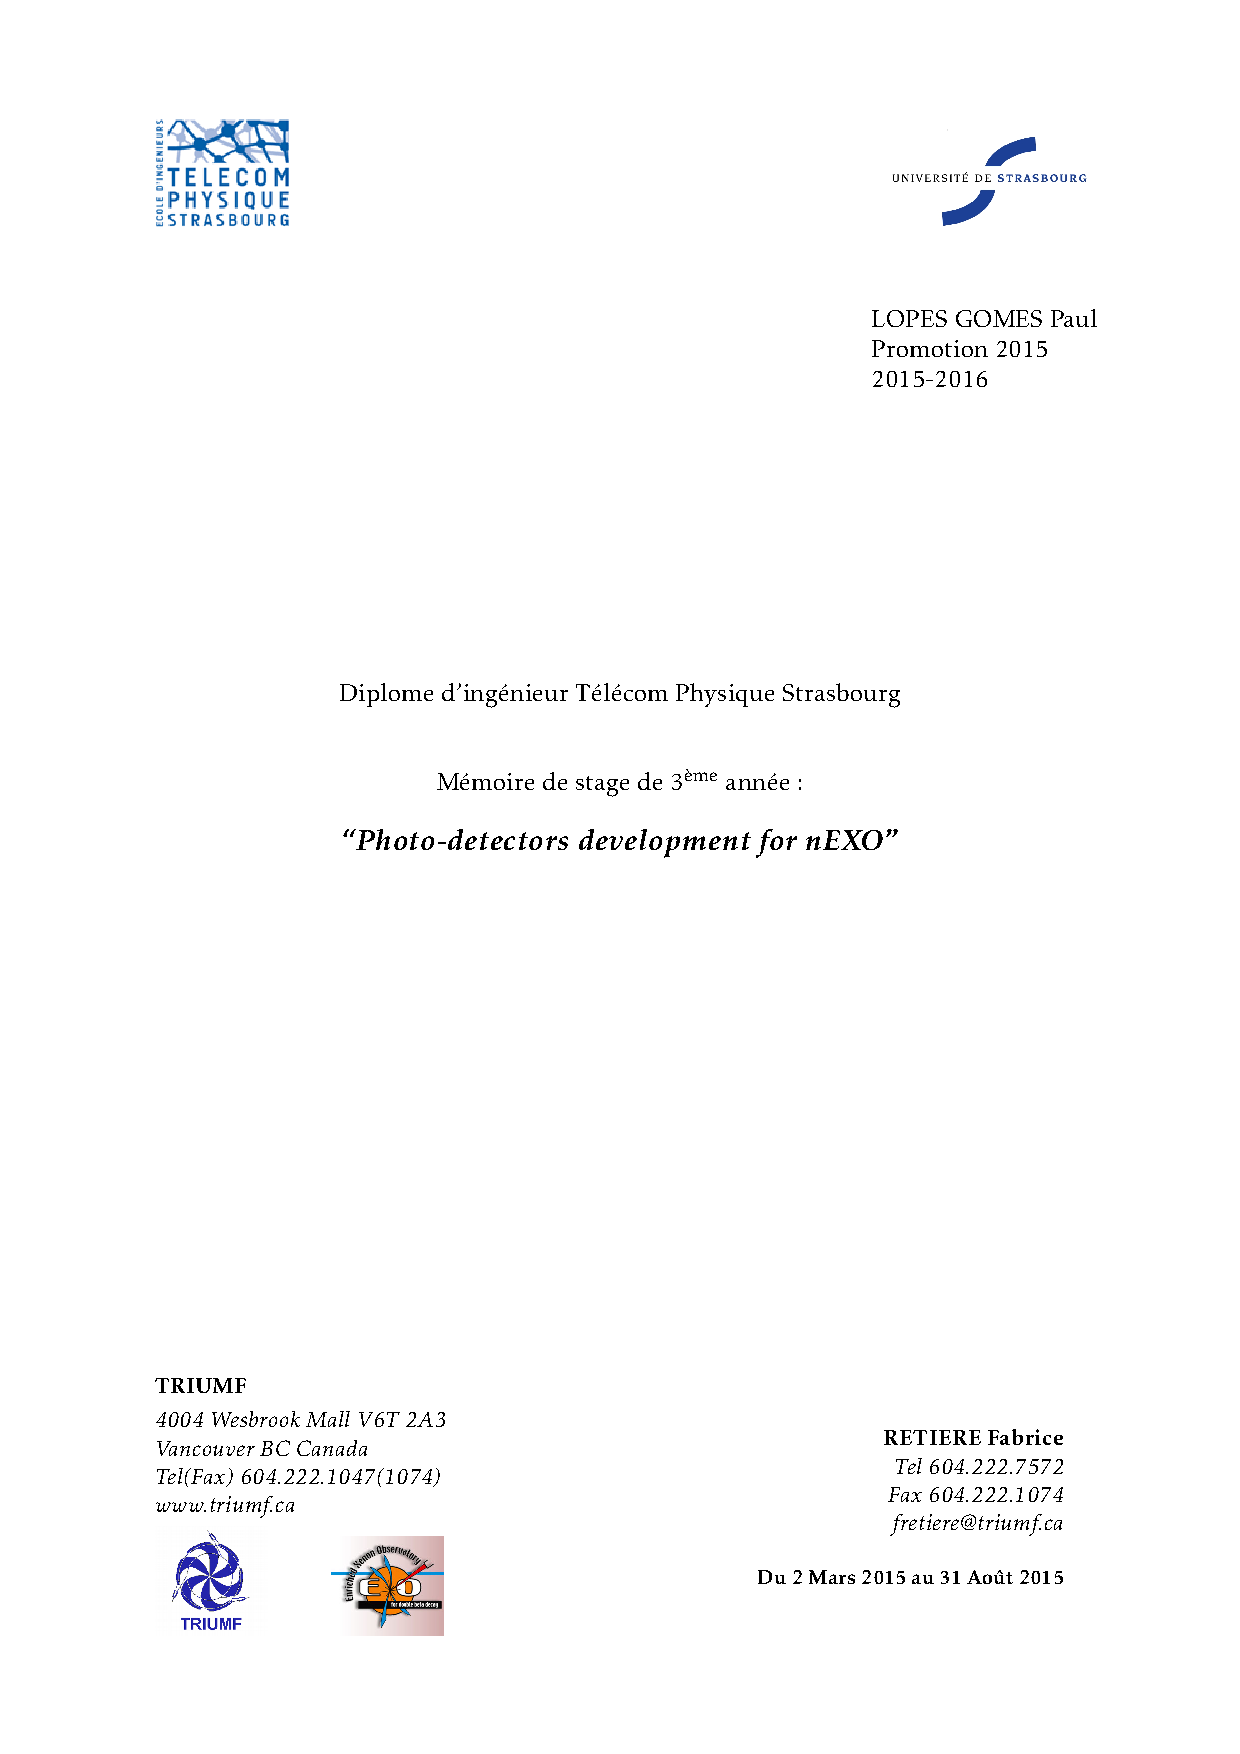
\includepdf{cover_page_TPS.pdf}


%%%%%%%%%%%%%%%%%%%%%%%%%%%%%%%%%%%%%%%%%%%%%%%%%%%%%%%%%%%%
%              a page to say thank you                     %
%%%%%%%%%%%%%%%%%%%%%%%%%%%%%%%%%%%%%%%%%%%%%%%%%%%%%%%%%%%%
\setcounter{page}{1}
\pagenumbering{roman}
\newpage
\thispagestyle{empty}



\vspace{1cm}
\paragraph{Thanks}\hspace{1cm}
  
  First I would like to express my gratitude towards \TR, a national laboratory for particle and nuclear physics, for having welcomed 
  me for those past 25 weeks of internship. I would like to thank especially Mr. Fabrice RETIERE who supervised the work of my team. 
  \\ 
  
  Many thanks to Ms. M. MCKAY, head of \TR's human resources. She helped me to come in Canada and guided me towards 
  \TR during my first days.
  Many thanks also for Mr. P. Lu, Mr. C. CHAMPMAN and Mr. C. LIM for their technical advises about the setup of my internship.
  \\
  
  I would like to thank in general each person who made this internship a real academical, professional and human succeed.\\ %contributed
  Many thanks especially towards my co-workers : Ms. E. TONITA, Mr. C. RETHMEIER and Mr. L. JAMES. I thank also 
  some students from Ottawa's University : Jaqueline, Chriss and Mathiew.
  \\
  
  Finally I thank Ms. A.S. CORDAN, Mr. S. LECLER and Mr. J. BAUDOT for their advices and their guidance from the beginning of my internship
  to my final defense for the master PSA.
  \\

%%%%%%%%%%%%%%%%%%%%%%%%%%%%%%%%%%%%%%%%%%%%%%%%%%%%%%%%%%%%
%                        Abstract                          %
%%%%%%%%%%%%%%%%%%%%%%%%%%%%%%%%%%%%%z%%%%%%%%%%%%%%%%%%%%%%%

\newpage
\thispagestyle{empty}

\paragraph{Abstract}\hspace{0.5cm}\\
  
  Founded in 1968 and located on the campus of UBC \footnote{University of British Columbia}, \TR \footnote{Canada's 
  national laboratory 
  for particle and nuclear physics} is one of the world's leading subatomic physics laboratories. Different research experiments in particle physics
  are conducted. On the microscopic scale \TR and nEXO \footnote{next generation Enriched Xenon Observatory} work together to measure 
  the neutrino-less double beta decay.\\
  \ce{^{136}Xe} may produce such a decay, emitting light at 175 nm. My internship focuses on the characterization of Silicum Photo-Multipliers which will be 
  used to detect this light in the nEXO experiment. To characterize them, efficiency, dark noise, crosstalk and after pulses are calculated
  at different over-voltages at $-100^\circ$C.\\
  Results for efficiency are inconsistent because of the initial misalignment of the beam of light coming from a \xfl with the surface of  
  photo-detectors. This effect gets 
  worst while the temperature of our setup is cooling down (because of a cooling system). Nevertheless a photo-detector produced 
  by HAMMAMASTU -VUV3 SiPM- shows a dark 
  noise rate less than around 12 Hz/mm\textsuperscript{2} at $-100^\circ$C and the average number of correlated pulses (crosstalk and after pulses)
  is less than 0.2 per parent pulses at 5 over-voltage for such a temperature. If the efficiency for such a photo-detector needs to be investigate, previous 
  results show
  this device as a good candidate for nEXO.  
  
  \paragraph{R\'esum\'e}\hspace{0.5cm}\\
   
   Fond\'e en 1968 et localis\'e sur le campus de l'UBC, \TR -Laboratoire national Canadien pour la recherche en physique nucl\'eaire et en physique des 
   particules- est l'un des plus importants laboratoires de physique subatomique au monde. Ce laboratoire est \`a la pointe de la recherche
   dans plusieurs domaines dont celui de la physique des particules. 
   A l'\'echelle nanom\'etrique \TR et nEXO travaillent ensemble \`a la recherche de la d\'esint\'egration b\^eta sans 'emission
   de neutrino.\\ 
   Si l'\'el\'ement chimique \ce{^{136}Xe} est un candidat potentiel pour produire une telle d\'esint\'egration avec \'emission de lumi\`ere \`a 175 nm, le but de mon 
   stage est de caract\'eriser des photod\'etecteurs au silicium (SiPM). De tels d\'etecteurs seront ensuite utilis\'es par l'exp\'erience nEXO 
   pour capter la lumi\`ere
   (photons) \'emise. Mesurer l'efficacit\'e quantique de ces detecteurs, le bruit thermique par unit\'e de surface milim\'etrique, 
   le nombre moyen
   d'impulsions d'interf\'erence et le nombre moyen de post-implusions ont \'et\'e effectu\'e à $-100^\circ$C.\\
   Les r\'esultats de l'efficacit\'e quantique ne sont pas reproductibles car le faisceau de la lampe au X\'enon n'est pas align\'e avec 
   la surface des photod\'etecteurs.Cet effet s'amplifie au fur et \`a mesure que la temp\'erature diminue.\\
   Cependant un photod\'etecteur de HAMMAMATSU -VUV3 SiPM- pr\'esente des propri\'et\'ees int\'eressantes pour l'exp\'erience nEXO: 
   le bruit thermique par unit\'e de surface ainsi que le nombre d'impulsions li\'ees \`a une impulsion primaire (impulsions d'interf\'erence et post-impulsions) 
   sont respectivement moins de 12 Hz/mm\textsuperscript{2} et moins de 0.2 par implusions primaires pour un exc\`es de tension de 5V. 
   Si l'efficacit\'e quantique doit \^etre 
   \'etudi\'ee, ce 
   photod\'etecteur est d\'ej\`a un bon candidat potentiel pour l'exp\'erience neXO.
   
     
   
%%%%%%%%%%%%%%%%%%%%%%%%%%%%%%%%%%%%%%%%%%%%%%%%%%%%%%%%%%%%
%                     contents page                        %
%%%%%%%%%%%%%%%%%%%%%%%%%%%%%%%%%%%%%%%%%%%%%%%%%%%%%%%%%%%%

\thispagestyle{empty}
\tableofcontents 



%%%%%%%%%%%%%%%%%%%%%%%%%%%%%%%%%%%%%%%%%%%%%%%%%%%%%%%%%%%%
%                     figures page                         %
%%%%%%%%%%%%%%%%%%%%%%%%%%%%%%%%%%%%%%%%%%%%%%%%%%%%%%%%%%%%

\thispagestyle{empty}
\listoffigures

%%%%%%%%%%%%%%%%%%%%%%%%%%%%%%%%%%%%%%%%%%%%%%%%%%%%%%%%%%%%
%                chapter 1 Introduction                    %
%%%%%%%%%%%%%%%%%%%%%%%%%%%%%%%%%%%%%%%%%%%%%%%%%%%%%%%%%%%%

\chapter{Introduction}


%%%%%%%%%%%%%%%%%%%%%%%%%%%%%%%%%%%%%%%%%%%%%%%%%%%%%%%%%%%%
%                 page number in arabic                    %
%%%%%%%%%%%%%%%%%%%%%%%%%%%%%%%%%%%%%%%%%%%%%%%%%%%%%%%%%%%%
  \setcounter{page}{1}
  \pagenumbering{arabic}
  
  This internship of 25 weeks is the last session of teaching that \TPS offers to its students to complete their 
  engineering studies. \\
  The goal of this internship for the student is to show that he is able to conduct a real engineering or research 
  work. 
  He's also asked to manage a project, to take its responsibilities and to show autonomous at work. 
  \\

  The subject of this internship covers the two main parts of teaching at \TPS. I was asked to have some knowledges both in electronics, 
  waveform processing or codding and also in particle and matter physics.The Master of Subatomics and Astroparticle Physics gave me bases on
  particles physics and also on physics about detectors. 
  \\ 
  
  This report is addressed to next students who will continue our work and also to people interesting in the subject of my internship.\\ 
  This report will describe first the laboratory \TR and the project on which I have worked. Then I will show the whole work that my team 
  and I did. At least I will concluded and I will give some recommendations for the next students who may continue our work. 
  \\
  
  At the end of that document some appendixes give more details about precises parts of that research project and allow the reader to 
  go deeper in understanding of the subject.

  
  \vfill
  
  keywords: Photo-detector, SiPM, efficiency, dark noise rate, after pulses and crosstalk. 
%%%%%%%%%%%%%%%%%%%%%%%%%%%%%%%%%%%%%%%%%%%%%%%%%%%%%%%%%%%%
%        chapter 2 a short abstract about \TR   3 pages    %
%%%%%%%%%%%%%%%%%%%%%%%%%%%%%%%%%%%%%%%%%%%%%%%%%%%%%%%%%%%%

\chapter{A short abstract about \TR}

  I worked at \TR from the beginning of April 2015 to the end of August 2015.
  
  \section{History and Partners}

  \subsection{History}
  
  \TR is one of the world' s leading subatomic physics laboratories and is considered Canada's leading nuclear science research institute. 
  \TR was founded in 1968 by a consortium of four universities whose the University of British Columbia (UBC).The goal was to provide a 
  research needs in particle physics. This laboratory is located on the campus of the University of British Columbia since 1971. 
  It was built around a cylcotron and the first beam of particles was produced in 1974.
  
  \begin{figure}[!hbtp]
  \centering
    
    
    \color{blue}\frame{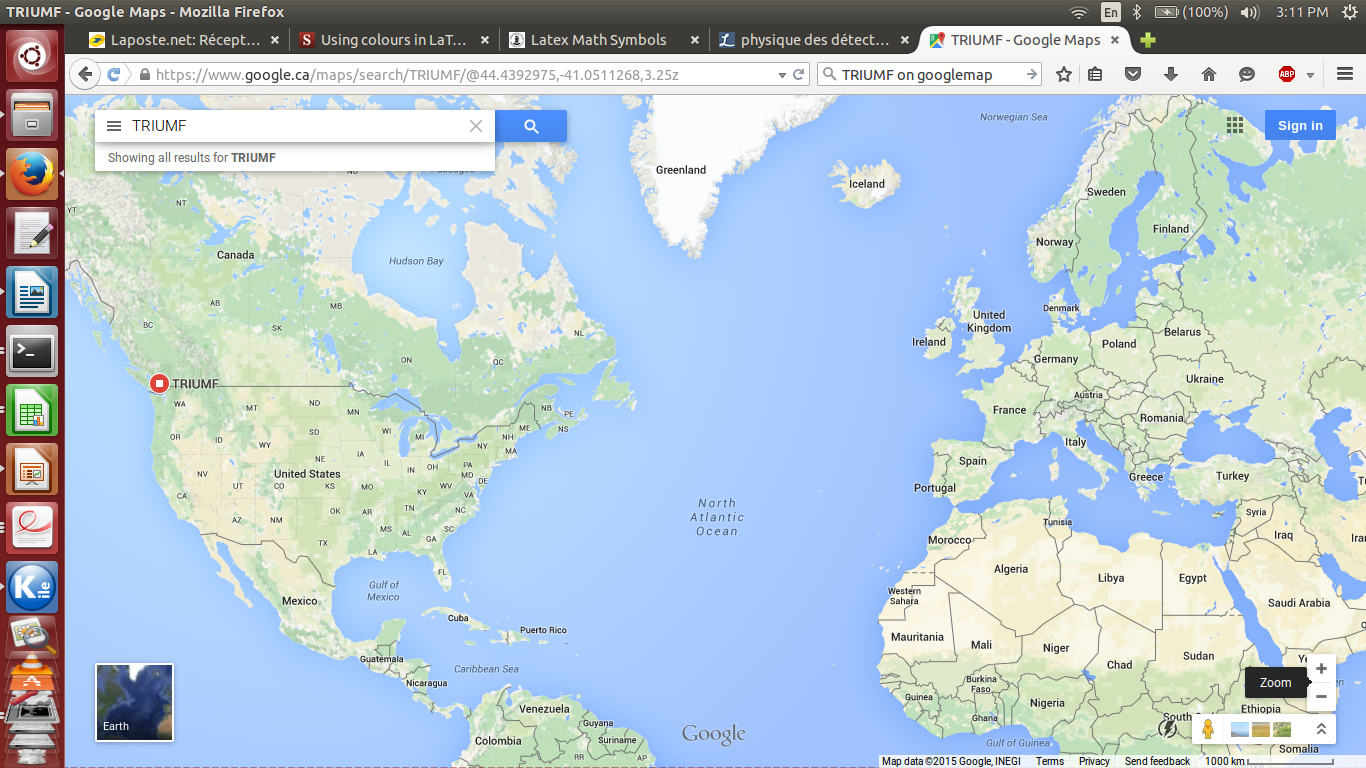
\includegraphics[trim=4cm 5cm 0cm 7cm, clip=true, totalheight=0.3\textwidth]{../Pictures/triumf_location.png}};

    \caption{\color{black}\TR on the  globe.}
    \label{fig:\TR_localisation}
  \end{figure}
  
  Over the year \TR has increased its research topics from the early cyclotron ERA (1965-1986) to medical science since 2009. 
  Four main steps reflect current researches conducted at \TR  thanks to the accelerator facilities:
  \begin{itemize}
   \item Nuclear Physics,
   \item Particle Physics,
   \item Material Sciences
   \item Medical Sciences. 
  \end{itemize}

  \subsection{Partners}
  %enlarges
  As no single university could provide research needs, the initial consortium grows up to 19 different 
  members and associate universities from across Canada. This consortium rules \TR and has allowed it to evolve into a national 
  laboratory.  
  \\
  
  \TR provides the centralized resources, tools, and expertise for its different Canadian partnerships. These partnerships could be 
  brought together in three different groups: 
  \begin{itemize}
  \item Canadian universities partners,  
  \item International partners whose GANIL \footnote[1]{Le Grand Acc'el'erateur National d'Ions Lourds} (Caen) and ISN (Grenoble) \footnote[1]{Institut des Sciences Nucl'eaires} in France,   
  \item Commercial partners. 
  \end{itemize}
  
  \section{Governance and Organization}
  
  Even if \TR is a laboratory, it could be considered like an enterprise that includes on-site technical, engineering , research and 
  administrative staff. Indeed \TR hosts more than 350 scientists, engineers, and staff performing research. Moreover this laboratory attracts over 
  500 national and international researchers every year and provides advanced research facilities and opportunities to 150 students and 
  postdoctoral fellows each year.
  \\
  
  \TR is a mix of material and human resources which allow conducting researches in total autonomous. For example the main parts of 
  our setup are designed and made at \TR. 
  \\
    
  \TR is organized to optimally meet its objectives while maintaining accountability, quality, and effectiveness. In that way this 
  laboratory is divided in eight different divisions, whose the Science Division. 
  \\
  
  Science Division is responsible for scheduling experiments approved by the 
  Experimental Evaluation Committee (EEC). This division is also responsible for all components of all systems and subsystems both for all 
  experimental operations at the \TR site and for other infrastructure for external programs whose nEXO.\\ 
  Dr. Fabrice RETIERE is the head of nEXO experiment :
  
  \newpage
  
  \begin{figure} [!hbtp]
    \centering    
    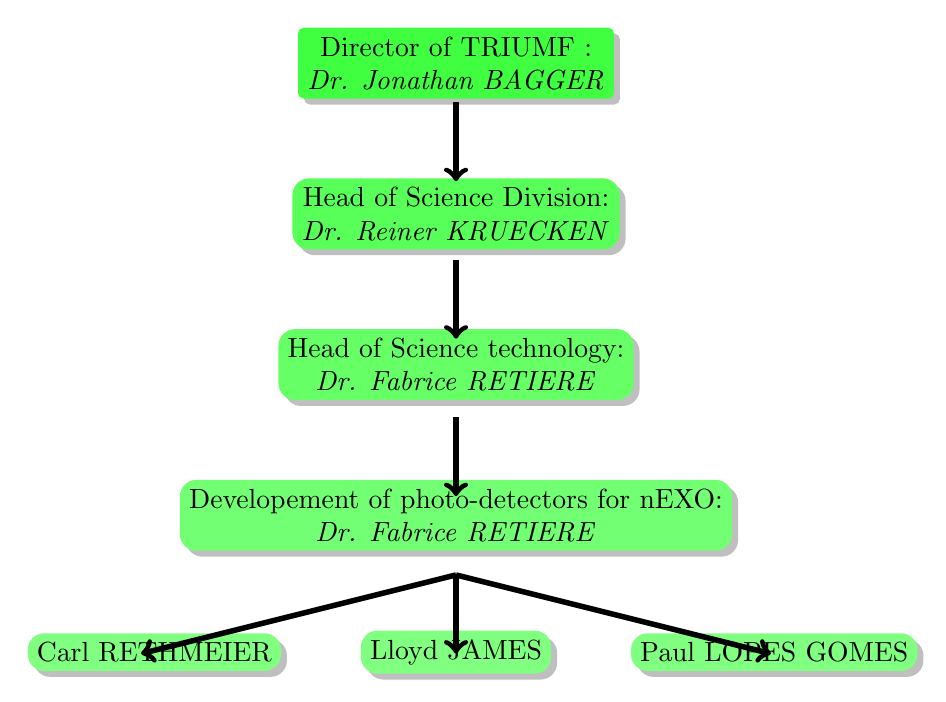
\begin{tikzpicture}[level 5/.style={sibling distance=40mm}, edge from parent/.style={->,draw, line width=1pt }]
      %order has importance
      \node[root] (root) {Director of \TR:\\ \textit{Dr. Jonathan BAGGER} };
      
      \node[level 1, below=of root] (level_1) {Head of Science Division:\\ \textit{Dr. Reiner KRUECKEN}};      
      \node[level 2, below=of level_1] (level_2) {Head of Science technology:\\ \textit{Dr. Fabrice RETIERE}} ;
      \node[level 3, below=of level_2] (level_3) {Developement of photo-detectors for nEXO:\\ \textit{Dr. Fabrice RETIERE}};
      \node[level 4, below=of level_3] (lloyd) {Lloyd JAMES};
      \node[level 4, left= of lloyd] (carl) {Carl RETHMEIER};
      \node[level 4, right=of lloyd] (paul) {Paul LOPES GOMES};
      
      \draw[->,black,line width=2pt] (0,-0.5) -- (0,-1.5);
      \draw[->,black,line width=2pt] (0,-2.5) -- (0,-3.5);
      \draw[->,black,line width=2pt] (0,-4.5) -- (0,-5.5);
      \draw[->,black,line width=2pt] (0,-6.5) -- (0,-7.5);
      \draw[->,black,line width=2pt] (0,-6.5) -- (4,-7.5);
      \draw[->,black,line width=2pt] (0,-6.5) -- (-4,-7.5);
  
  \end{tikzpicture}
  \caption{Organisation chart from the Head of \TR to our work team.}
  \label{fig:organigram}
  \end{figure}

    
   
  \section{Research topics at \TR}
  
  As a publicly-funded national laboratory, TRIUMF's activities are framed within its mission and vision with a strategic plan developed 
  every five years. The Government of Canada and other agencies review, approve and finance research experiments.\\
  The strategic plan of \TR could be divided in three main parts : 
  
  \begin{itemize}
  \item The advancing isotopes for science and medicine,  
  \item The harnessing particles and beams for discovery and innovation,   
  \item The understanding of the building blocks of matter and how they shape our universe. 
  \end{itemize}

  Seven different research topics are conducted at \TR: from nuclear medicine to the investigations in theory group 
  through the particle physics. 
  \\
  
  These programs exploit the opportunities provided by TRIUMF's core facilities.\\
  The driving motivation behind particle physics experiments is the desire to uncover the true nature of fundamental forces and particles. 
  Our current standard model \cite{ref:modern_particle_physics} believes to be an effective theory, which has a deeper underlying theory 
  \footnote{\textit{Physics beyond the Standard Model}} reachable in the next generation of experiments.
  \\
  
  For example in particle physics, in the electroweak sector \cite{ref:modern_particle_physics} successes of the past 
  decades have predicted and verified the unification of the electromagnetic and weak nuclear forces.\\
  More recently precision measurements at the CERN large electron positron collider (LEP) 
  and the Fermilab proton-antiproton collider (Tevatron) demand that there be either a light Higgs particle with a mass less 
  than about 200 GeV or a physical system mimicking its interactions. 
  \\
  
  On the atomic scale ($10^{-9}$) SNOLAB' s experiment focuses on the discovery of neutrinoless double-beta decay which will prove the theory 
  \textit{Physics beyond the Standard Model}.
  
  \paragraph{\underline{\textit{From SNOLAB to EXO-200}}}
  \leavevmode
  \\
  
  SNOLAB' s experiment places it center stage in two quests on opposite scale : on the cosmic scale for interstellar dark matter and on the 
  microscopic scale for neutrinoless double-beta decay. 
  \\
  
  On the cosmic scale astrophysical measurements indicate that $80\%$ of the matter in the universe is ``missing'', which means
  that this matter does not emit any heat or light. This matter is called dark matter.\\
  Experiments at SNOLAB will search for hypothesized rare interactions between dark matter and normal matter. On the microscopic end of 
  the spectrum, neutrinoless double beta decay probes the very nature of antimatter.\\
  Advanced theories of particle physics and the Big Bang suggest that the neutrino particle may have a special nature: it might be its 
  own antiparticle \cite{ref:majorana_fermions}.\\
  Answering this question about the neutrino could give light for future researches on the cosmic scale. 
  \\
  

%%%%%%%%%%%%%%%%%%%%%%%%%%%%%%%%%%%%%%%%%%%%%%%%%%%%%%%%%%%%
%    chapter 3 presentation fo the subject 4/5 pages       %
%%%%%%%%%%%%%%%%%%%%%%%%%%%%%%%%%%%%%%%%%%%%%%%%%%%%%%%%%%%%

\chapter{Motivations}

  \section{Understand physical phenomena} 
  
  Human scale doesn't allow observing what matter is made. But it has been proved theoretically and by 
  experiment that matter is made of elementary particles \cite{ref:modern_particle_physics} predicted by the \textit{Standard Model}. 
  The most known elementary particle is the electron. Photon belongs also to that family of elementary particles and it is quiet known that 
  light has the properties of both a wave and a particle, called photon.\\
  The Standard Model divides that family of elementary particles in fundamental fermions and fundamental bosons:
  
%   \begin{tcolorbox}[tab2,tabularx={X||Y|Y|Y|Y},title=Elementary Particle,boxrule=0.5pt]\label{tab:elementary_particles}
% 	& Fermions & & & Bosons \\\hline\hline
% 	& I & II &  III &  \\\hline\hline
%   Quark & \Pup & \Pcharm &  \Ptop & \Pgg \\\hline
% 	& \Pdown & \Pstrange &  \Pbottom & \Pg \\\hline\hline
% 	& \Pnue & \Pnum & \Pnut & \PZ \\\hline
%   Lepton & \Pelectron & \Pmu & \Ptau & \PW \\\hline
%   \end{tcolorbox}
  
  \begin{figure}[!hbtp]
    \centering
    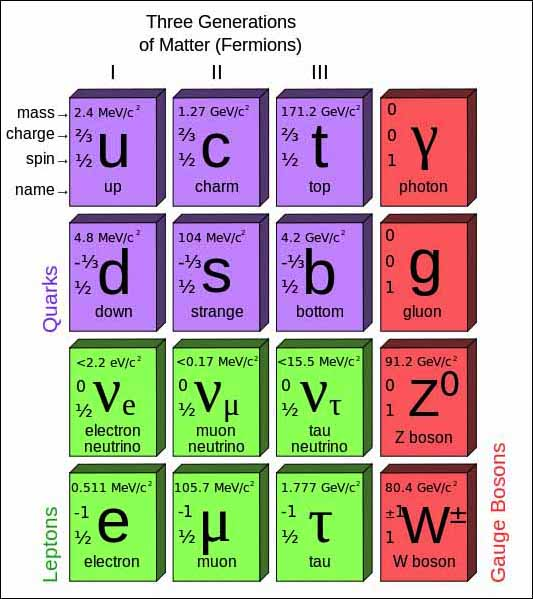
\includegraphics[trim=0cm 0cm 0cm 0cm, clip=true,totalheight=.5\textwidth]{../Pictures/StandardModelParticles.jpg}
    \caption{Elementary particles according to the \textit{Standard model}. The leptonic number of the $\Pelectron$ and the $\Pnue$ is +1 each while for their
    own anti-particle is -1 each.}
    \label{fig:elementary_particles}
  \end{figure}
  
  The Standard Model predicts also that antimatter is creating on the same time than matter, which means that  there are also 
  antiparticles which have the same mass as particles of ordinary matter but have opposite charge and other particle properties 
  such as the lepton number \ref{fig:elementary_particles}. 
  % ref ?????
  %Collisions between particles and antiparticles lead to the annihilation of both,
    
  Physical properties of particles and antiparticles such mass or energy can be calculated by using certain type of 
  detectors such as mass spectrometers or photo-detectors.
  
  \subsection{Is the neutrino a Majorana particle?}
  
  As it has been reminded above, electronic neutrinos and electronic antineutrinos are particles and antiparticles, respectively. \\
  A currently quest about neutrino is to check if neutrino has a certain characteristic which is to be a Majorana particle 
  \footnote{In opposition of Dirac particles where particles are distinct from anti-particles.}.
  The double beta decay (\(2\Pneutrino\beta\beta\)), predicted by the Standard Model, allows observing such a characteristic.
  \\
    
  $\ce{^{136}Xe}$ is one of the 35 natural isotopes capable of \(2\Pneutrino\beta\beta\).
  In such decay a nucleus with charge Z and mass number A \footnote{The mass number is the total number of nucleons (proton (Z) and 
  neutron (A-Z) within a nucleus} decays to a nucleus with charge Z+2 and mass number A, where both Z and A are even. We speak 
  about even-even nuclei.\\
  As two neutrons become in two protons, the conservation of the charge implies the creation of two electrons \ref{eq:charge}. As 2 electrons 
  appear, the conservation of the leptonic electronic number implies the creation of two anti-neutrinos \ref{eq:leptonic} (The leptonic
  number for electron and electronic anti-neutrino is given previously):
  
  \begin{equation} \label{eq:charge}
    (A,Z) \rightarrow (A,Z+2) + 2\Pelectron + 2\APneutrino
  \end{equation}
  
  leptonic electronic conservation :
  
  \begin{equation} \label{eq:leptonic} 
    0 \rightarrow 0 + 2*(+1) + 2*(-1)
  \end{equation}
  
  In case of $\ce{^{136}Xe}$ the double beta decay is : 
 
  \begin{equation}\label{eq:Xe_decay}
    \ce{^{136}Xe} \rightarrow \ce{^{136}Ba} + 2\Pelectron + 2\APneutrino %\iff 2\Pneutron \rightarrow 2\Pproton + 2\Pelectron \iff \ce{^{136}Xe} \rightarrow 2\APneutrino + 2\Pelectron 
  \end{equation}
 
  We could observe a single beta-decay instead, if there was not a peculiarity in the nuclear mass function of certain
  even-even nuclei. This is shown for the case of $\ce{^{136}Xe}$ \ref{fig:even_even_nuclei} where single beta-decay to $\ce{^{136}Cs}$
  is energetically disfavored over \(2\Pneutrino\beta\beta\) to $\ce{^{136}Ba^{++}}$.
 
  \newpage
  
  \begin{figure}[!hbtp]
  \centering
    \frame{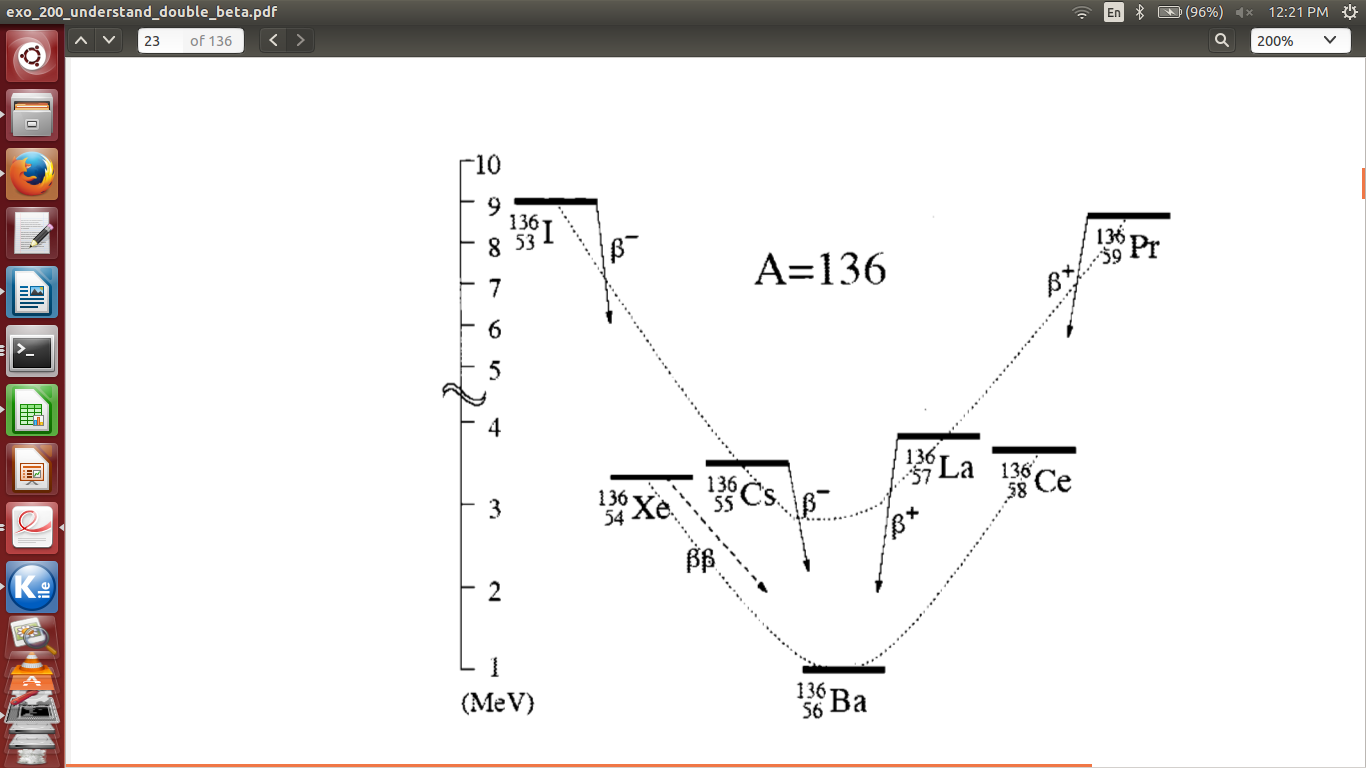
\includegraphics[trim=15cm 1.5cm 6cm 5cm, clip=true,totalheight=.45\textwidth]{../Pictures/xe_ba.png}}%trim=leftcm bottomcm rightcm topcm, clip=true, 
    \caption{Nuclei with A = 136. Parabola connecting ``odd-odd'' and ``even-even'' nuclei are shown. Single \(\beta\)-decay of 
    $\ce{^{136}Xe}$ to $\ce{^{136}Cs}$ is energetically forbidden.}
  \label{fig:even_even_nuclei}
  \end{figure}
  
  Now lets consider the case when neutrinos are Majorana particles which means neutrino and anti-neutrino are identical except 
  for their helicities \cite{ref:modern_particle_physics}. If so switching the helicity allows a neutrino to be an anti-neutrino.\\
  That means that the emitted anti-neutrinos is neutrinos which conducts to the equation:
  
  \begin{equation}
    \ce{^{136}Xe} \rightarrow \ce{^{136}Ba} + 2\Pelectron
  \end{equation}
  
  Such a decay releases lots of energy. The energy shares between the nuclei \ce{^{136}Ba} and the two electrons. 
  As the mass of the nuclei $\ce{^{136}Ba}$ is higher than the one of an electron \footnote{$\frac{Mass_{\ce{^{136}Ba}}}{Mass_{\Pelectron}} = 10^{7}$}, 
  we could consider, in first approximation, that 
  the $\ce{^{136}Ba}$ doesn't move and that the whole energy is transmitted into kinetic energy to the both electrons. 

  \subsection{From EXO-200 to nEXO}
  %In such barrel nucleus $\ce{^{136}Xe}$ will decay most of the case in double beta decay and also in neutrinoless doule beta decay 
  
  EXO-200 is a double beta decay experiment, employing 200 kg of liquid $\ce{Xe}$ (LXE) in a barrel, isotropically enriched to  $80\%$ 
  of $\ce{^{136}Xe}$ \footnote{Neutrons are added to $\ce{^{136}Xe}$ atoms. They are told to be in excess of neutrons in oder to observe the 
  beta radioactivity}.\\
  In such a barrel atoms of $\ce{^{136}Xe}$ will decay according to both the double beta decay and  
  the neutrinoless double beta decay (see previous section). 
  From such decays \ref{eq:Xe_decay} the two electrons are ejected with high kinetic energy and scatter off the electrons of other 
  $\ce{^{136}Xe}$ atoms.\\
  If so, one of the impacted $\ce{^{136}Xe}$ atoms is excited from the ground state and then de-energizes by releasing photons. 
  This is the scintillation process: 
  
  \newpage 
  
  \begin{figure}[!hbtp]
    \centering
    \frame{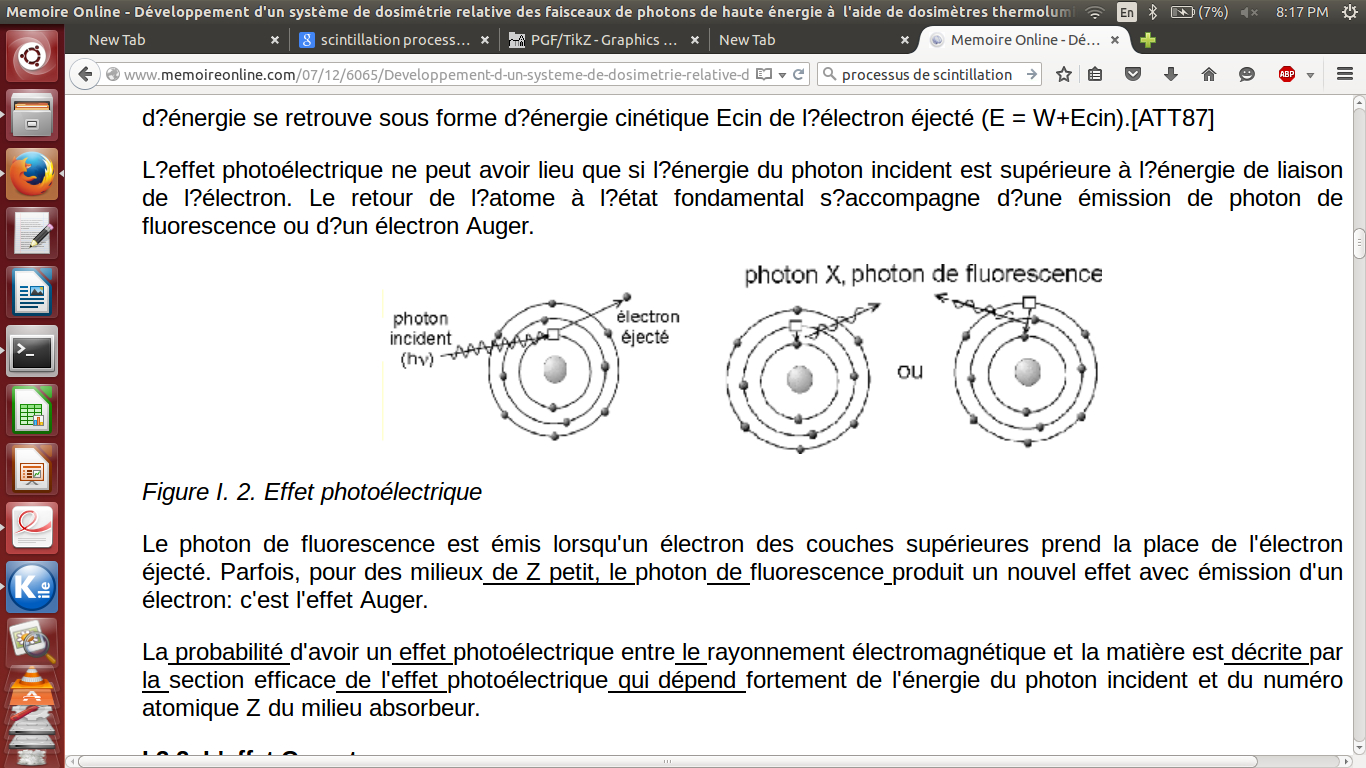
\includegraphics[trim=25cm 11cm 9cm 10.15cm, clip=true,totalheight=.3\textwidth]{../Pictures/scintillation_process.jpg}}%trim=10cm 4cm 1cm 12cm, clip=true, 
    \caption{Scintillation process: the excited atom releases its energy by emitting light (fluorescence photons).}
    \label{fig:scintillation}
  \end{figure}
  
  The scintillation energy of that light comes from \(2\Pneutrino\beta\beta\) or from \(0\Pneutrino\beta\beta\) and 
  EXO-200 experiment records this energy by using a type of photo-detector called Avalanche Photo-Diode (APD). 
  The results are plotting in graph showing 
  the scintillation energy versus the ionization energy \cite{ref:motivation_and_introduction}. The $Q_{\beta\beta}$ shows 
  the \(0\Pneutrino\beta\beta\) decay:
  
  \begin{figure} [!hbtp]
  \centering 
    \includegraphics[trim=0cm 2.15cm 12cm 4.8cm, clip=true,totalheight=.6\textwidth, page= 3]{../MotivationAndIntroduction.pdf}  
    \caption{nEXO will increase the resolution of the scintillation energy for the \(0\Pneutrino\beta\beta\).}
    \label{fig:scintillation_ionization}    
  \end{figure}
  
  A simple link between scintillation energy and ionization energy is given in that following equation:
  
  \begin{equation}
   E = Q_{d} + \frac{S_{d}}{\epsilon},
  \end{equation}
  
  where $E$, $Q_{d}$, $S_{d}$ and $\epsilon$ are the total energy detected, the ionization energy detected, the 
  scintillation energy detected and the efficiency of the APD.\\
  Thus a small variation of the total energy $\Delta E$ and the efficiency of the APD $\epsilon$ are linked according to that 
  equation: 
  
  \begin{equation}\label{eq:resolution}
    (\Delta E)^{2} = \sigma_{Q_{d}}^{2} + (\frac{\sqrt{S_{d}}}{\epsilon})^{2}
  \end{equation}

  Assuming that the scintillation energy detected is linked to the efficiency and to the initial scintillation energy 
  $S_{i}$:
  
  \begin{equation}
    S_{d} = S_{i}\epsilon
  \end{equation}
  
  the equation \ref{eq:resolution} becomes:
  
  \begin{equation}
    (\Delta E)^{2} = \sigma_{Q_{d}}^{2} + \frac{S_{i}}{\epsilon}.
  \end{equation}
  
  From that last equation, we can see that the energy resolution $\Delta E$ is inversely proportional to the efficiency 
  of the photo-detectors. The table page 15 of that reference \cite{ref:motivation_and_introduction} draws a short 
  comparison between two different types of photo-detectors(Avalanche Photo-Diode and Silicum Photo-Multiplier):
  the efficiency of a SiPM is better than the one of an APD. 
  \\
  
  The next energy improvement will be to construct the nEXO experiment. This experiment is a collaboration of 
  19 universities or laboratories whose TRIUMF. nEXO is currently being designed to use 5 tons of enriched 
  liquid Xenon contained in a barrel (instead of 200 kg for EXO-200).\\
  The wall of this barrel will be covered with photo-detector SiPM.
    
  \subsection{The subject of my internship}
  
  The goal of my research internship is to identify suitable SiPMs for nEXO by testing devices from several manufacturers.\\
  In 2014 a test setup was built: a box divided in two parts. 
  The first part contains a \xfl which sends photons to the surface of two SiPMs. The signals are observed 
  on the screen of an oscilloscope, which is monitored by a computer. This computer allows registering and storing waveforms. 
  An algorithm (C++ and root) lets us characterize the SiPMs.
  \\
  
  The goal is to determine if a selected SiPM could fulfill all the nEXO experiment's requirements: 
  
  \begin{itemize}\label{item:conditions}
    \item Achieve efficiency \(\geq\)15\% at 175nm (the wavelength of Xenon scintillation light), 
    \item Achieve dark noise rate less than 50Hz/mm\texttwosuperior{}, 
    \item Limit the number of correlated pulses (crosstalk and after pulses) to less than 0.2 per parent pulse.
  \end{itemize}
  
  All of those requirements was done at $-100^{\circ}$C and in ultraviolet conditions (or VUV) in oder to stay as closer as possible to the 
  operating nEXO experiment (At $-100^{\circ}$C and wavelenght of 175 nm). 
  
  
%%%%%%%%%%%%%%%%%%%%%%%%%%%%%%%%%%%%%%%%%%%%%%%%%%%%%%%%%%%%
%               chapter 4 summarize of my work             %
%%%%%%%%%%%%%%%%%%%%%%%%%%%%%%%%%%%%%%%%%%%%%%%%%%%%%%%%%%%%

\chapter{SiPM Studies}
  
  \section{Methodology}
  
  I worked with 2 others students.  We divided the work according to our qualities and skills.
  \\
  
  So Carl and I thought about algorithms to analysis waveforms recorded from the oscilloscope. 
  As Carl had yet worked on SiPM before, he wrote mainly different programs to analysis them.
  Both of us tried to find also technical solutions for different issues we had.\\
  As I worked on the setup the first month of my internship, I was mainly responsible of the setup and of taking data.\\
  As Lloyd worked on the setup one year ago he wrote different programs for the automation stuff. He also wrote a function called 
  ``Pulsefinding.exe'' to calculate the dark noise and after pulses rate.\\
  Data analysis was made using C++ and ROOT. \\  
  This mix of knowledges allows finding technical solutions and thinking about algorithms. 
  \\
  
  As we were considered as members of the nEXO collaboration we were also able to give regularly talks about the advancement of 
  our work.
  
  \section{The Setup}
  
  The goal is to characterize, at $-100^{\circ}$C, photo-detectors receiving light from a xenon flash lamp. In 2014 a setup was built while taking 
  account the two main features of nEXO : working at $-100^{\circ}$C and the wavelength of the light from the \xfl should be 175 nm.\\ 
  The picture below \ref{fig:aluminum_box} shows an aluminum box divided into two parts. On the left side is a Xenon flash lamp and 
  on the right side are two photo-detectors. \\
  The photo-detector on the top is used as reference. It allows checking if the light from the lamp reminds constant over time. It also let calculate
  the absolute efficiency of the photo-detector on the bottom \ref{sec:PE}.
  The one on the bottom is characterized and a system allows cooling it.     
  
  \newpage
  \begin{figure}[!hbtp]
    \centering
    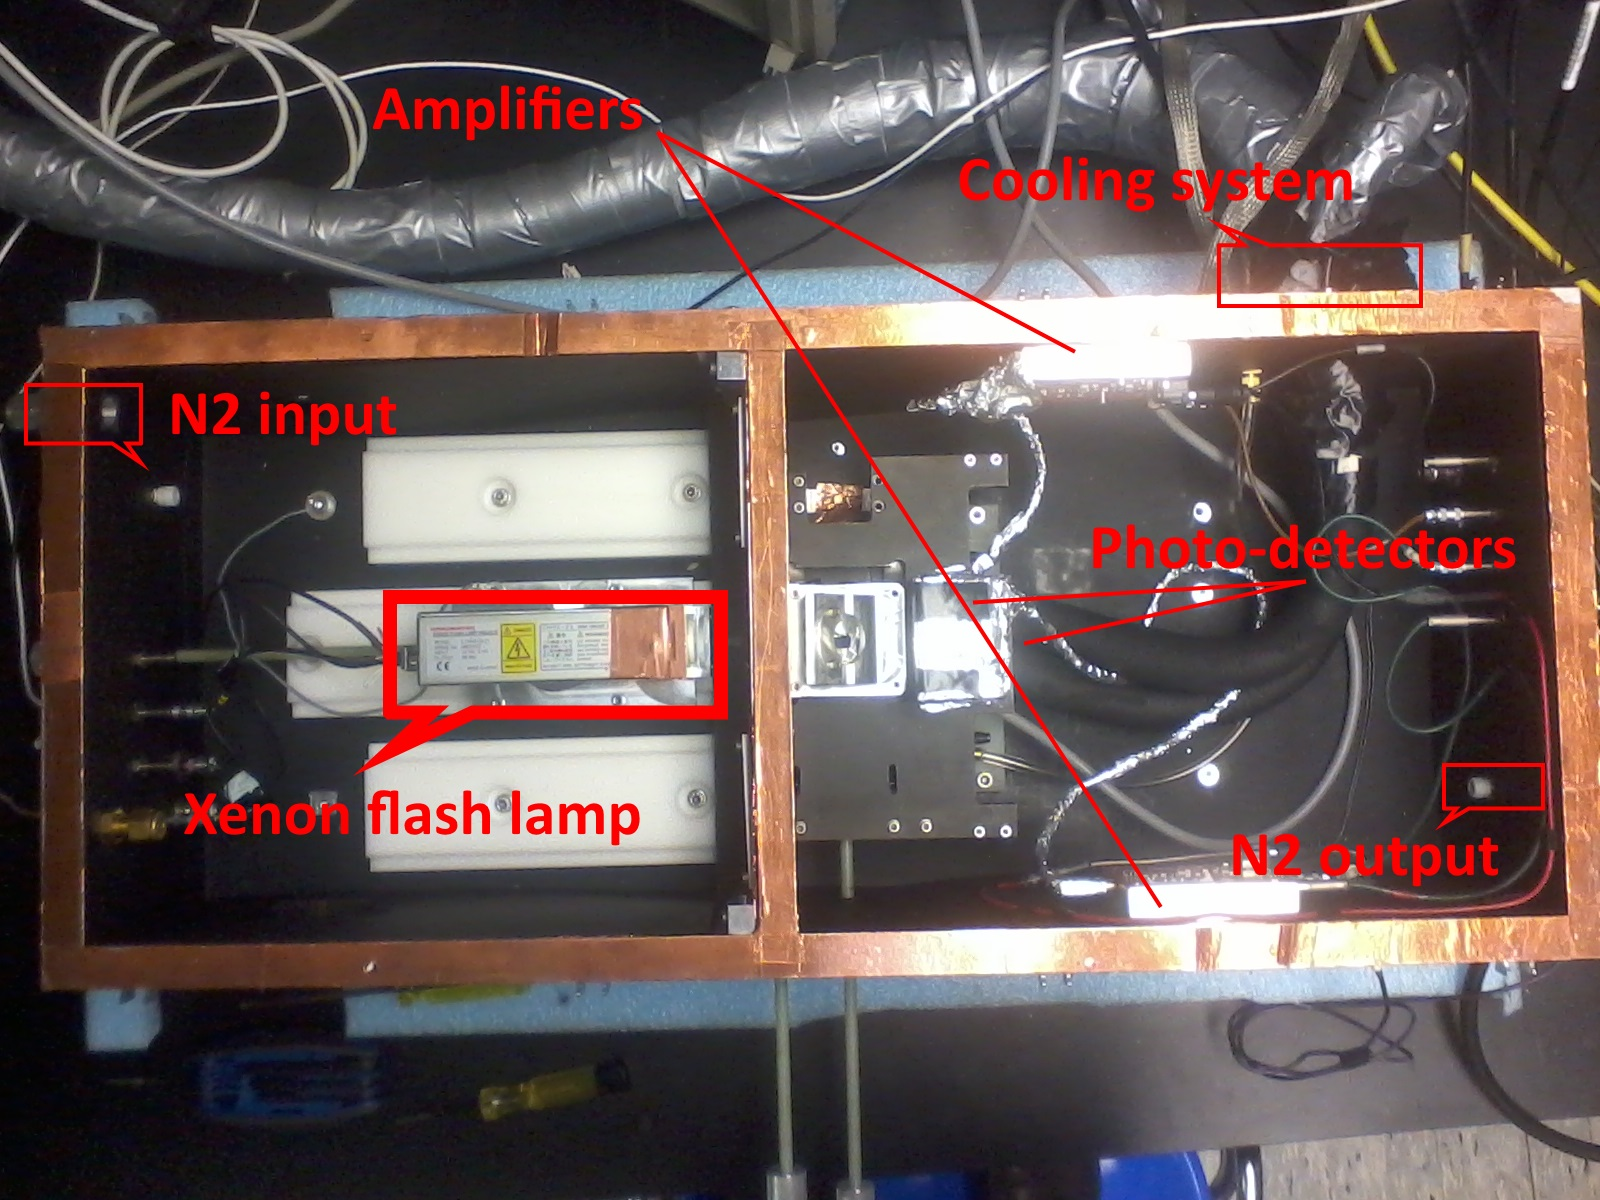
\includegraphics[totalheight=.38\textwidth,trim=0cm 7cm 0cm 2.5cm, clip=true]{../Pictures/blabla/box.jpg}%trim=10cm 4cm 1cm 12cm, clip=true, 
    \caption{An aluminum box contains a \xfl and two photo-detectors.}
    \label{fig:aluminum_box}
  \end{figure}
  
  The reader will find more informations and pictures about the setup in the appendix \ref{app:setup}. 
  
  \subsection{The \xfl}
  
  A Hamamatsu L11035-03-21 Xenon flash lamp module is used as a light source in a nitrogen-filled, light-tight box to simulate 
  the ultraviolet conditions (VUV) of the future experiment. 
  The amount of light hitting the photo-detectors is managed by a square wave pulse generator, otherwise saturation of the signal 
  from the photo-detectors occurs. 
  \\
  
  To control light output, and thus the number of photons reaching the photo-detectors, we could move out the lamp away from the 
  area of the detectors
  since intensity of light drops off as one over distance squarred. 
  We could also set the voltage discharge on the lamp by adding an external voltage supply line. 
  
  \begin{figure}[!hbtp]
  \centering
    \begin{subfigure}[The voltage of the lamp is set by this external supply line.]{%
      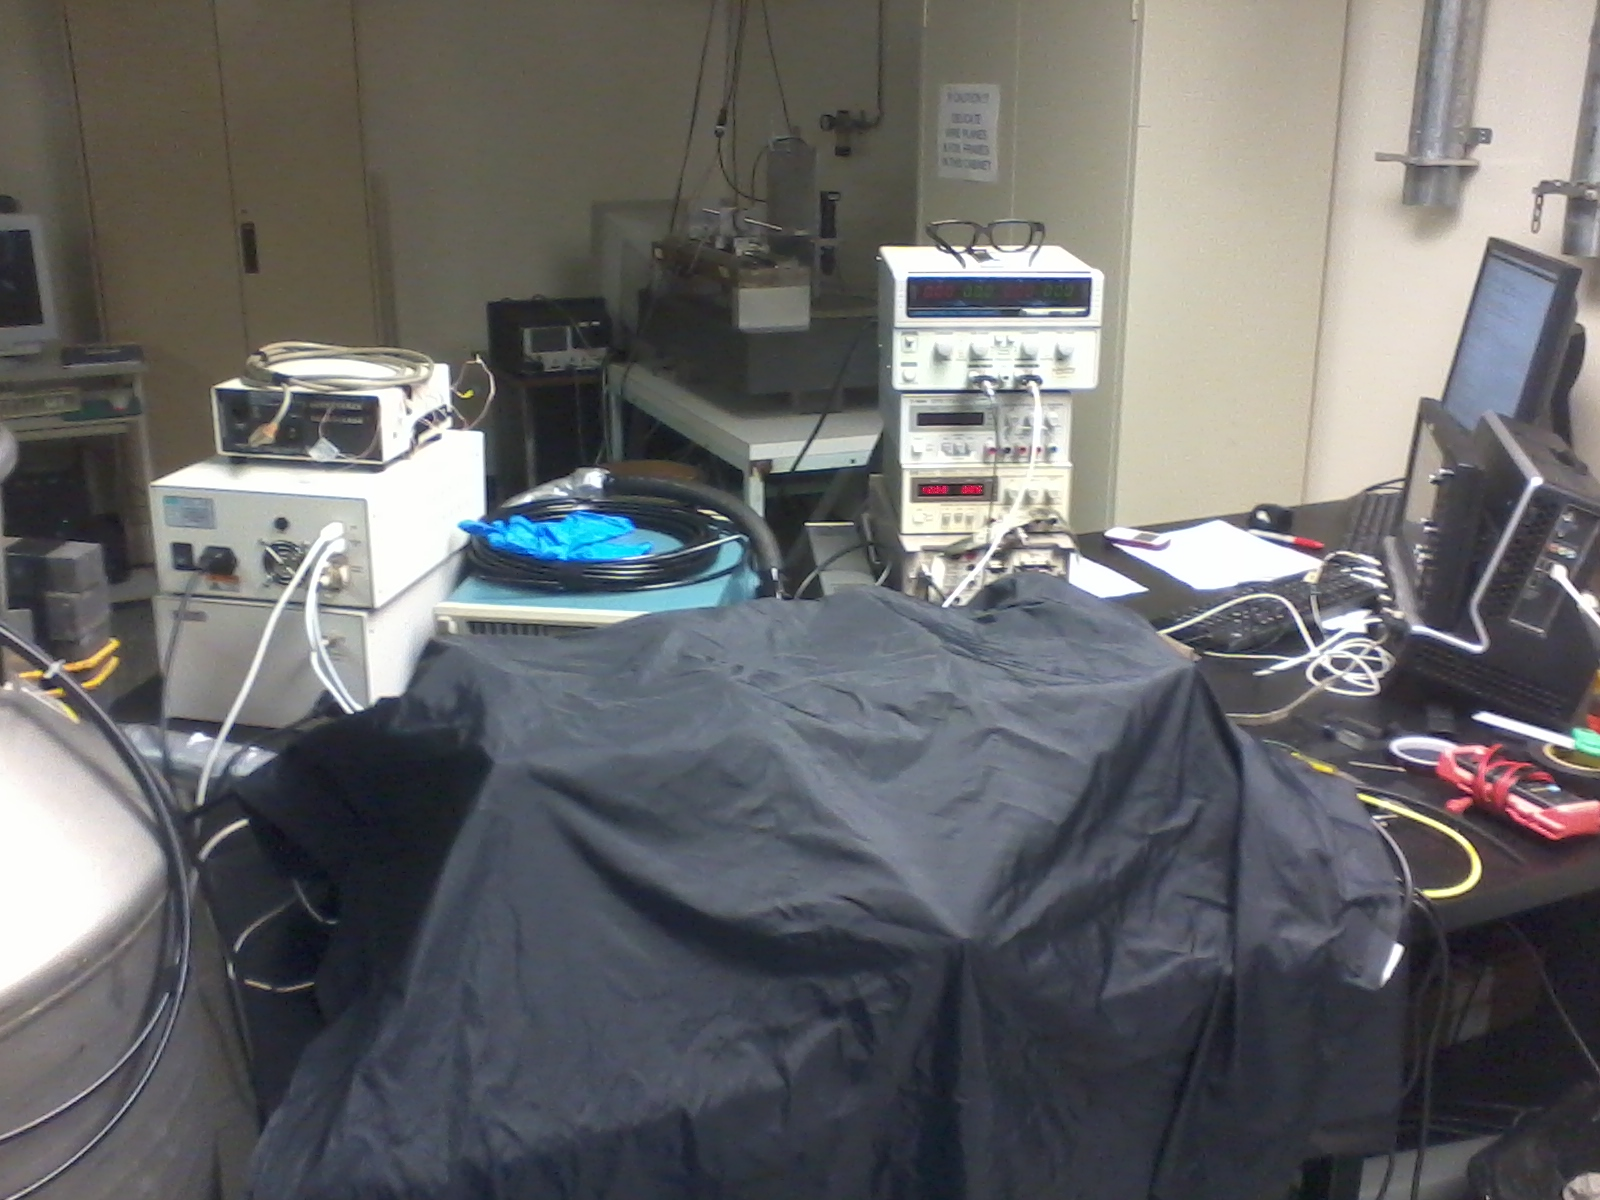
\includegraphics[width=.4\textwidth,trim=30cm 28cm 15cm 8.65cm, clip=true]{../Pictures/Pictures_Setup/external_voltage.jpg}
      \label{fig:external_voltage}}
    \end{subfigure}
  \quad  
    \begin{subfigure}[A pulse generator controls the frequency (10 ms) and the duration of each flash of the lamp (10$\Pmu$s). 
		      The frequency of the lamp is limited by the reading speed of the oscilloscope (20 GHz maxi).]{%
      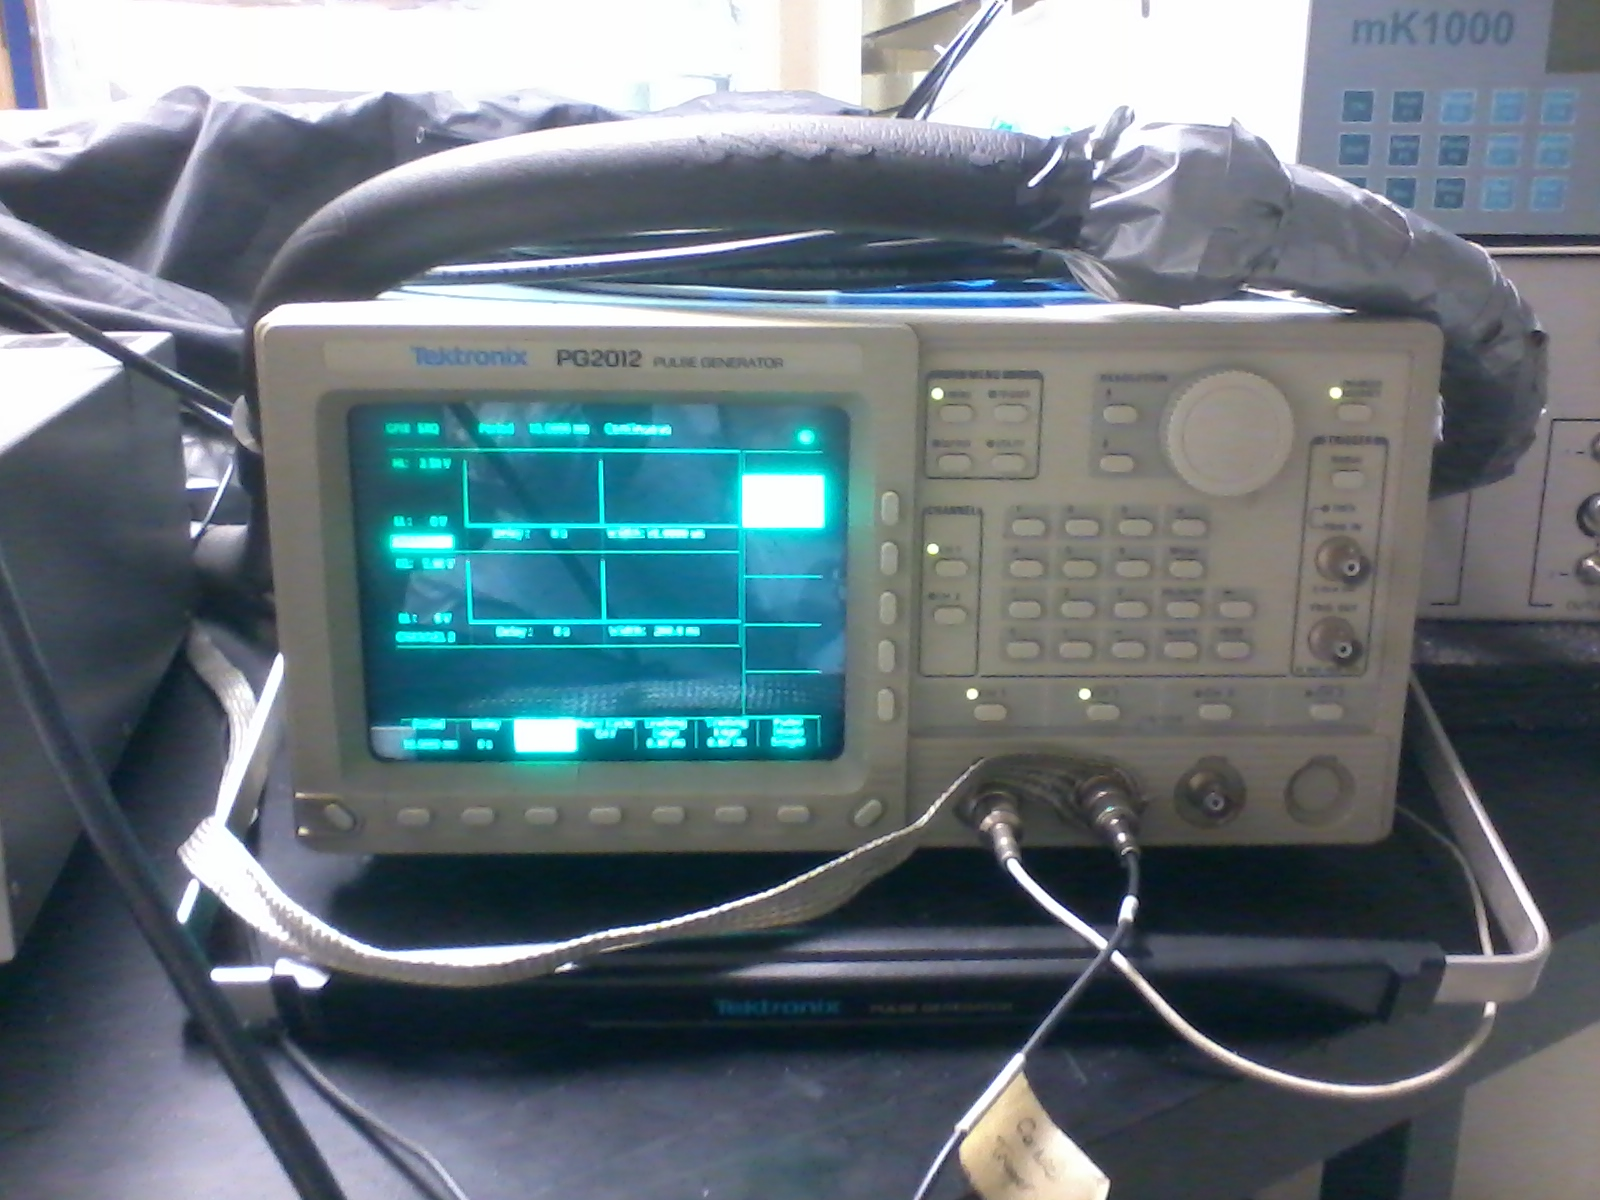
\includegraphics[totalheight=.2\textwidth,trim=8.5cm 12cm 5cm 10cm, clip=true]{../Pictures/Pictures_Setup/pulse_generator.jpg}
      \label{fig:pulse_generator}}
    \end{subfigure}
  \caption{Devices to control the \xfl}
  \label{fig:device_lamp}
  \end{figure} 
  
  Then the light was collimated by a 5 mm hole, filtered, and then interacts with a beam splitter (BS). The beam splitter separated 
  the incoming beam of 3 mm diameter into two 
  equal beams which reached the surface of each photo-detector on the same time. 
  
  \newpage 
  
  \begin{figure}[!hbtp]
  \centering
    \begin{subfigure}[The incoming beam reaches the surface of each detectors due to the beam splitter.]{%
      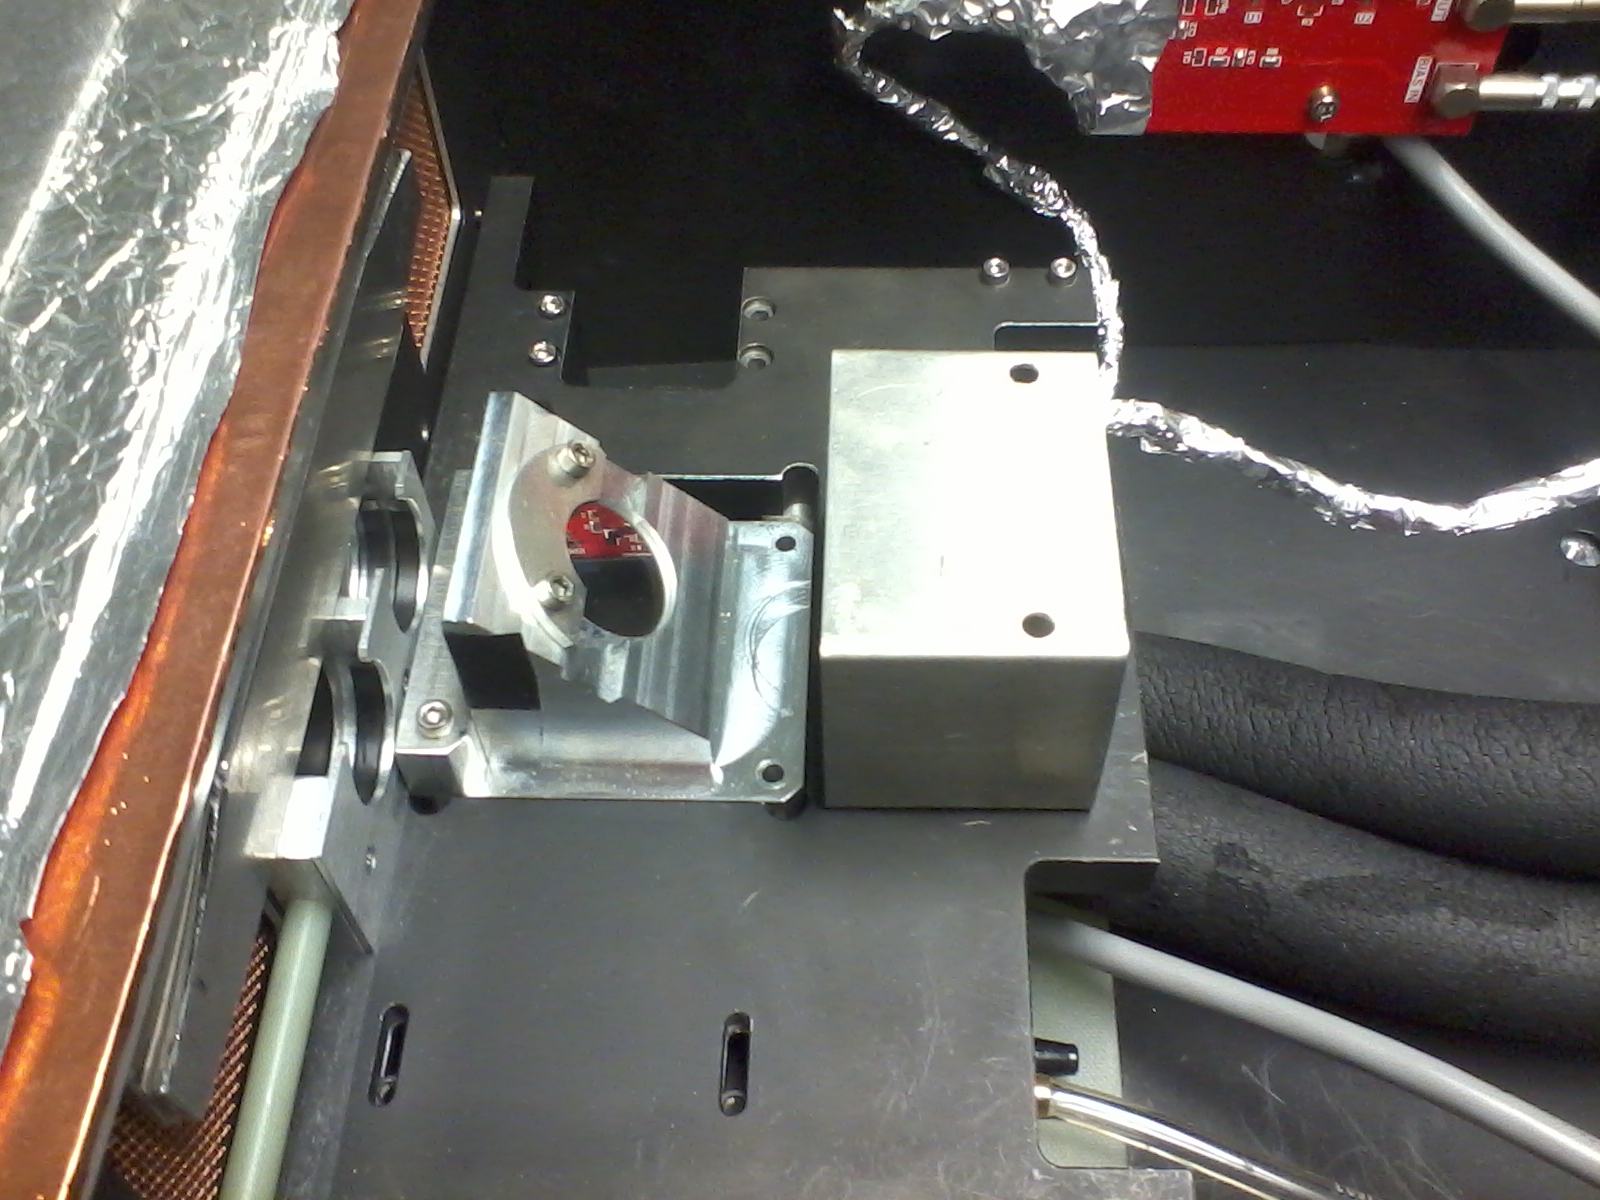
\includegraphics[width=.368\textwidth,trim=14.5cm 12cm 25cm 13cm, clip=true]{../Pictures/Pictures_Setup/beam_splitter.jpg}
      \label{fig:beam_splitter}}
    \end{subfigure}
  \quad  
    \begin{subfigure}[The filter in front of the lamp select the VUV region. Both of them attenuate the light of around 20$\%$ each.]{%
      \begin{tikzpicture}
      \node (img) {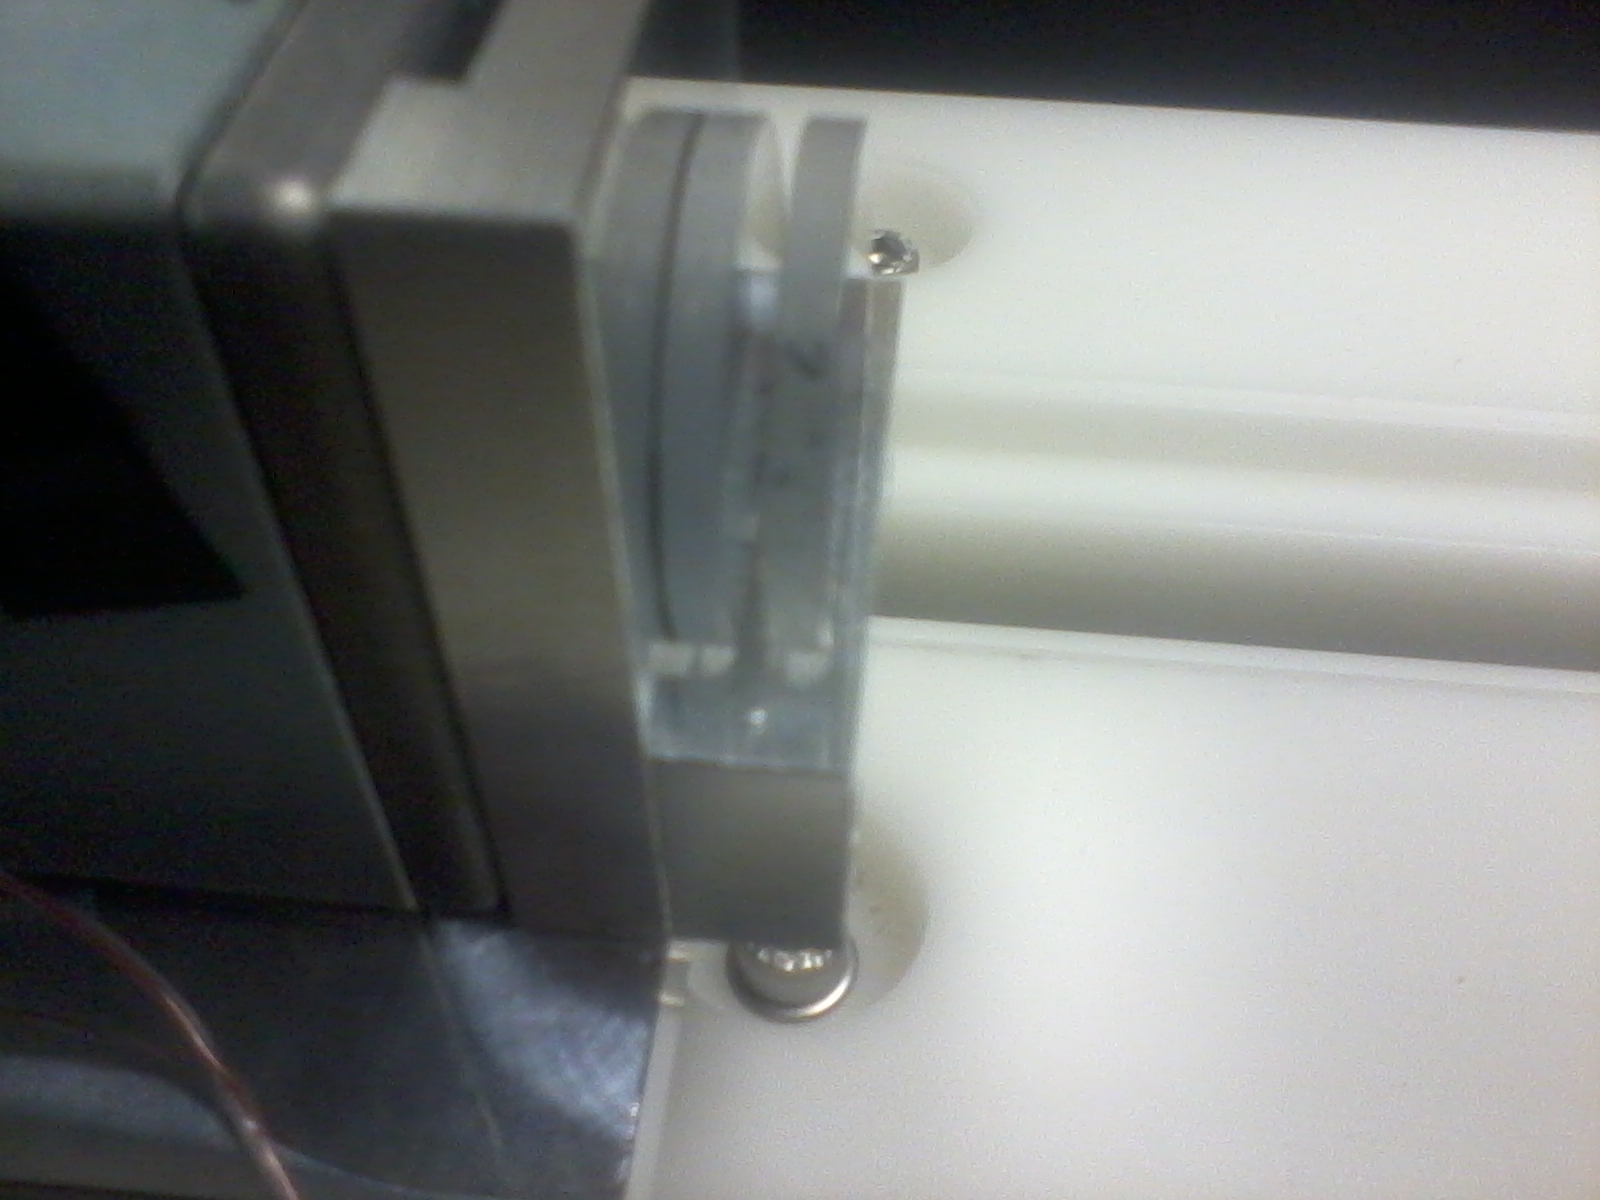
\includegraphics[width=.495\textwidth,trim=0cm 0cm 0cm 0cm, clip=true]{../Pictures/Pictures_Setup/filter_2.jpg}};
      %\node at ( -pt,-50pt) {\color{red} $Filter$};
      \end{tikzpicture}
      \label{fig:filter}}
    \end{subfigure}
  \caption{Beam splitter and filters}
  \label{fig:bs_filter}
  \end{figure}
  
  To select the 175 nm wavelength (VUV region) a filter is added in front of the lamp \ref{fig:filter}. 
  A test was made to ensure that no visible light from that lamp could reach the photo-detectors sensitive to the visible 
  wavelength (Otherwise such light could have got wrong our results for the efficiency).\\
  This filter also attenuates the light of the \xfl by $20\%$ and that expected attenuation was checked: we found $18.79\%$. 
  The run is described in the appendix \ref{app:tests}.\\. 
  Then two other identical filters are added before the incoming light reaches the beam splitter (the intensity of the light is too high). 
  We also noticed that the photo-detector
  on the bottom receives more light than the one on the top. That means that the inclination of the beam splitter is more
  than $45^{\circ}$. An additional filter is added on the bottom.
  \\
  
  As photons of this wavelength have an attenuation length of only a few mm in oxygen, the box was filled with N2 gas. 
  The second advantage of using N2 is to avoid frost on the surface of the cooling photo-detectors on the bottom.
  \\
  
  Also the appendix \ref{app:setup} or informations provided by HAMMAMATSU \cite{ref:\xfl} gives the pulse shape of the lamp. We can 
  notice that the pulse shape last around 140 ns  and the relative light output reaches $100\%$ after 400 ns. The time of 1.4 $\Pmu$s
  is seen on the screen of the oscilloscope \ref{app:tests}. 
  
  \newpage
  
  \begin{figure}[!hbtp] 
    \centering
      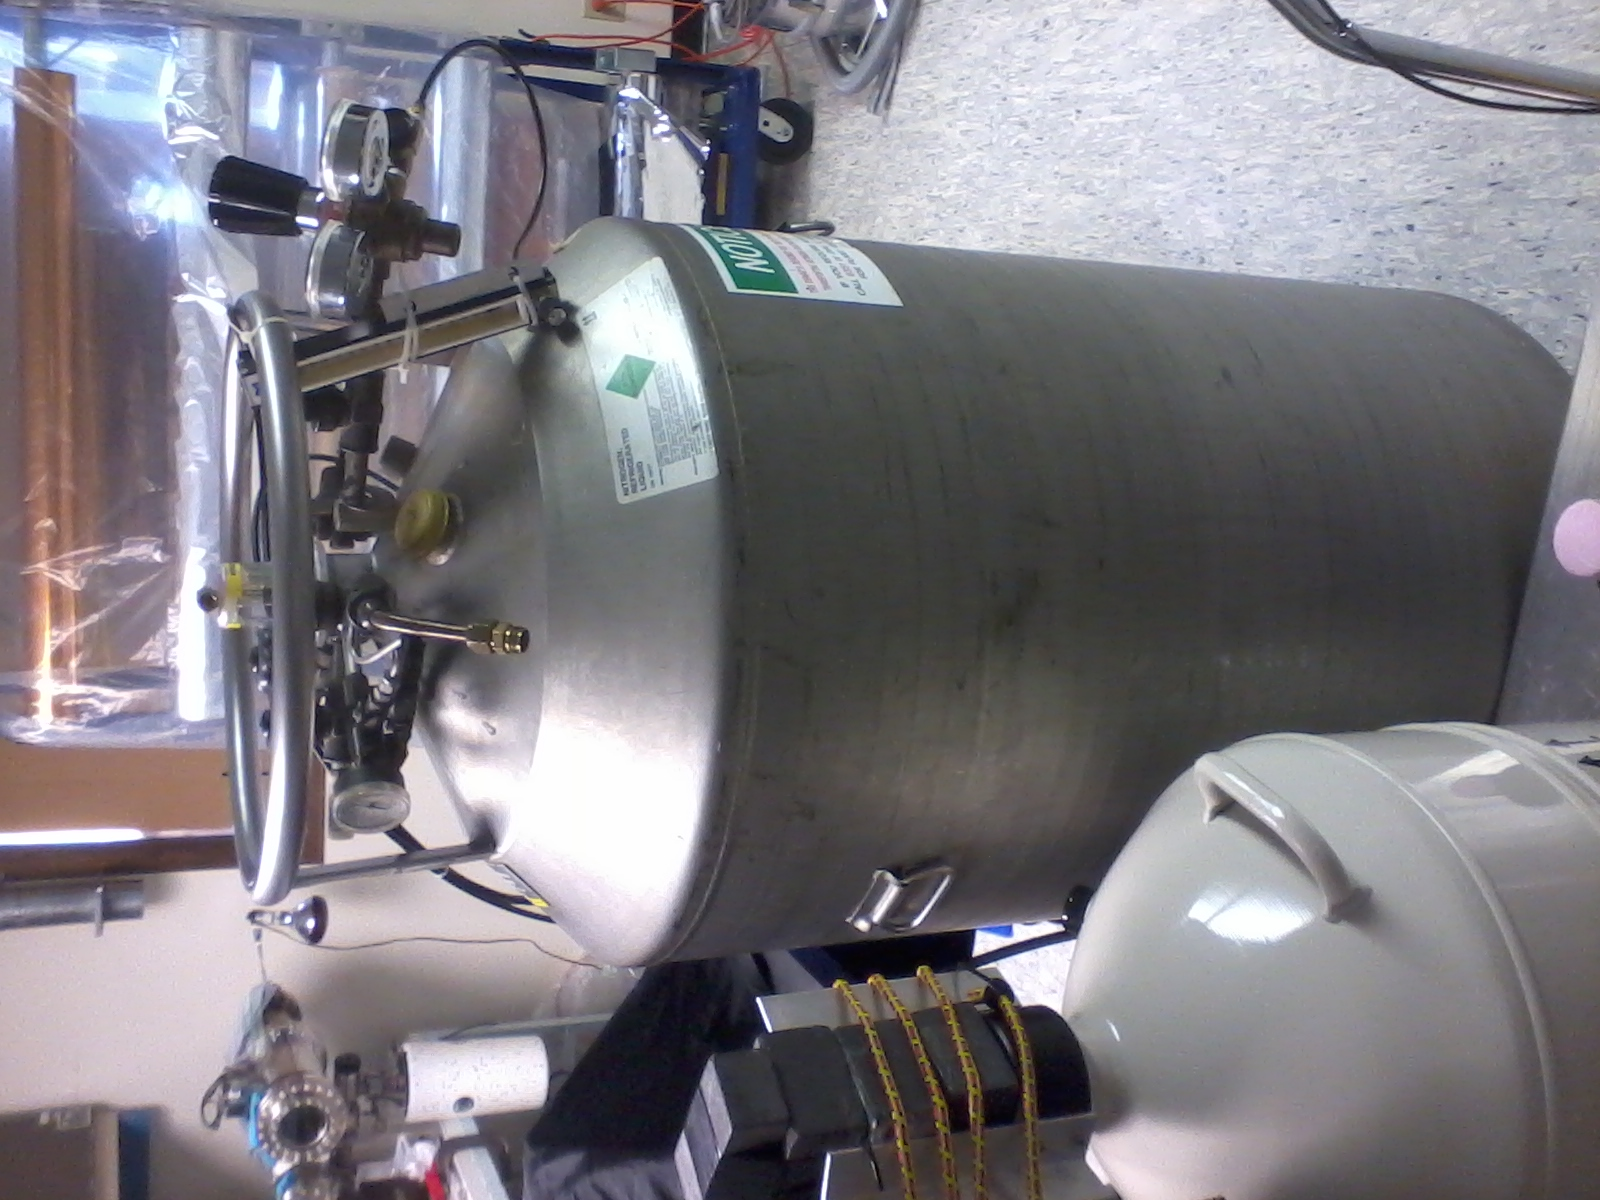
\includegraphics[totalheight=.35\textwidth, angle=270,trim=05cm 7.8cm 1cm 1cm, clip=true]{../Pictures/Pictures_Setup/N2_fills_box.jpg}
      \caption{N2 from that bottle fills the box.}
      \label{fig:N2_fills_box}
  \end{figure}
  
  
  \subsection{Photo-detectors and the cooling system}
  
  Two photo-detectors were used for each run to calculate the efficiency.\\
  The one on the top allow ensuring that the light reminds constant over the time. For that we used a VUV2 SIPM from HAMMAMATSU.
  
  
  \begin{figure}[!hbtp] 
    \centering
    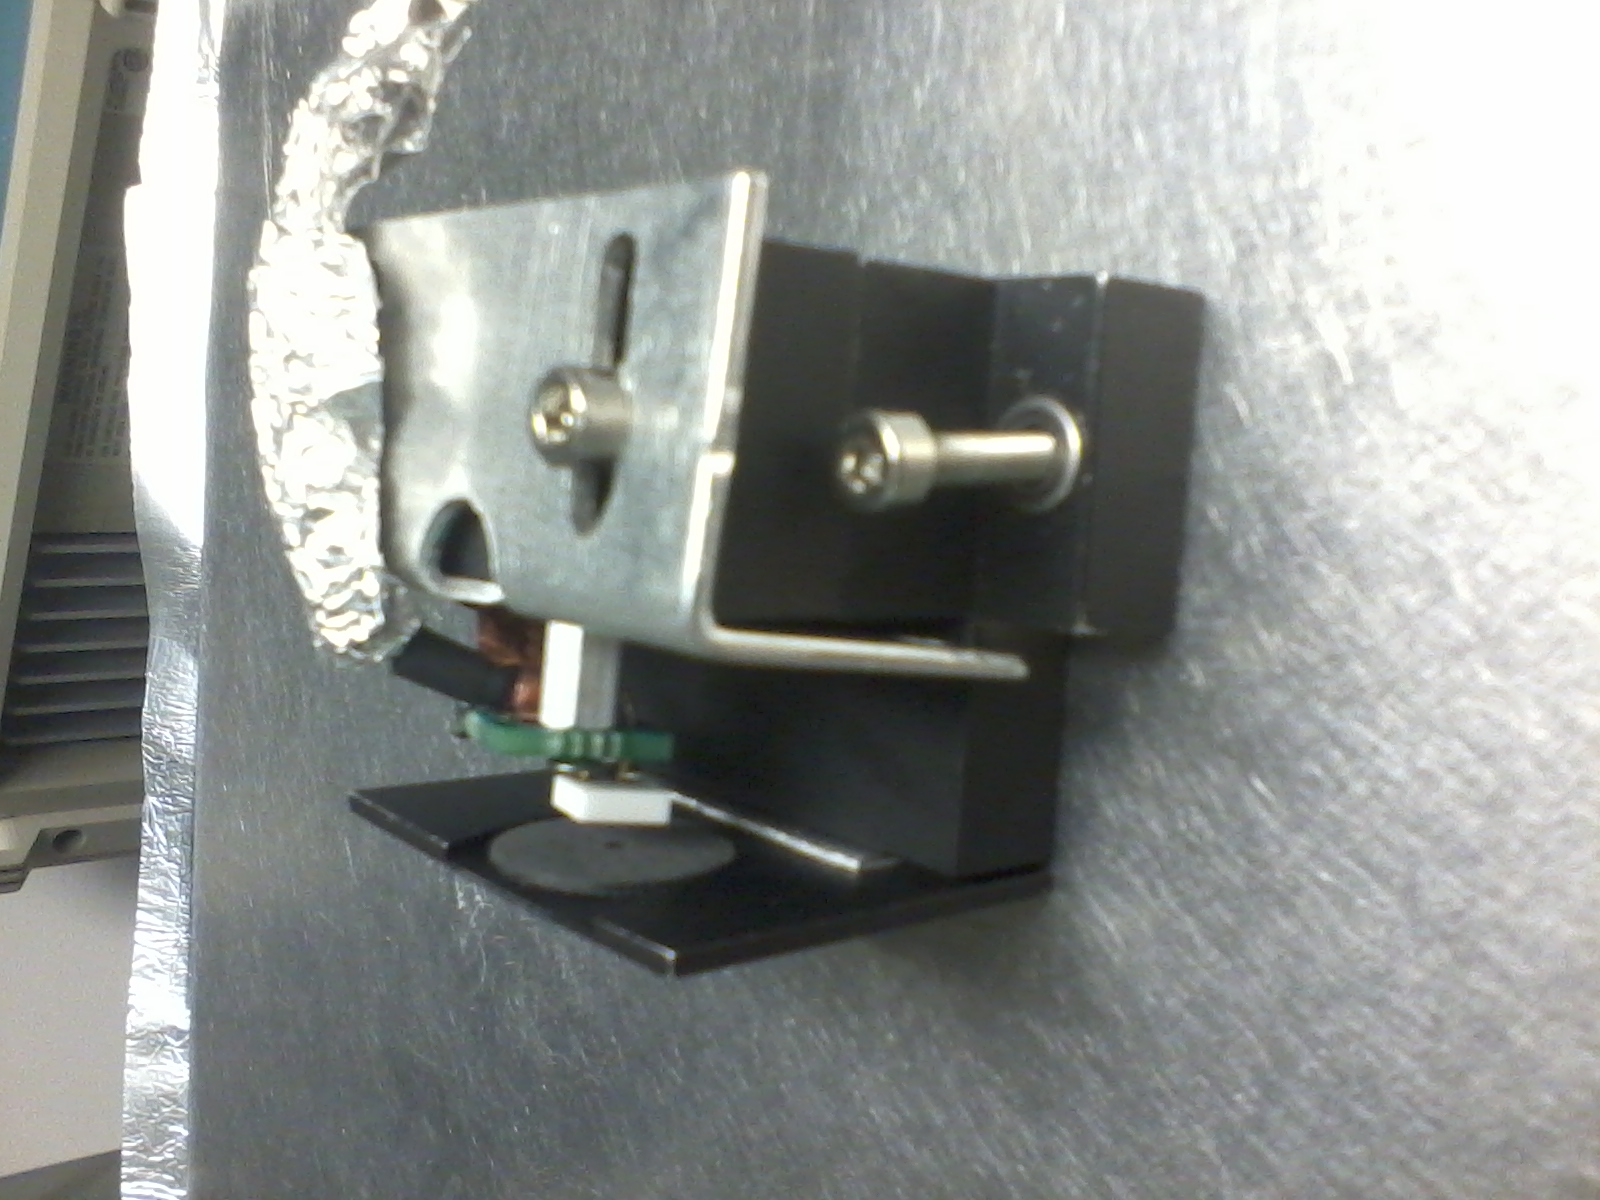
\includegraphics[totalheight=.35\textwidth,angle=270, trim=8cm 7cm 12cm 3.5cm, clip=true]{../Pictures/Pictures_Setup/VUV2_top.jpg}
    \caption{A VUV2 SiPM on the top lets check if the light from the lamp is constant.}
    \label{fig:top}
  \end{figure}
   
  We chose such a detector because the dark noise rate \ref{sec:DN} is quiet low at room temperature (~$20^{\circ}C$). So it is possible 
  to calculate the relative efficiency of that detector at such temperature. \ref{sec:PE}.
  \\
  
  The photo-detector on the bottom were characterized (calculate the efficiency at $-100^{\circ}$C, the dark noise rate and the number of 
  correlated pulses).\\
  A cooling system allows working at such a low temperature and the photo-detector to characterize was laying on a shock. A plastic board 
  with low thermal conductivity holds the whole cooling shock to avoid thermal leaks.
  
  
  \begin{figure}[!hbtp]
  \centering
    \begin{subfigure}[The cooling system lets work up to $-110^{\circ}$C.]{%
      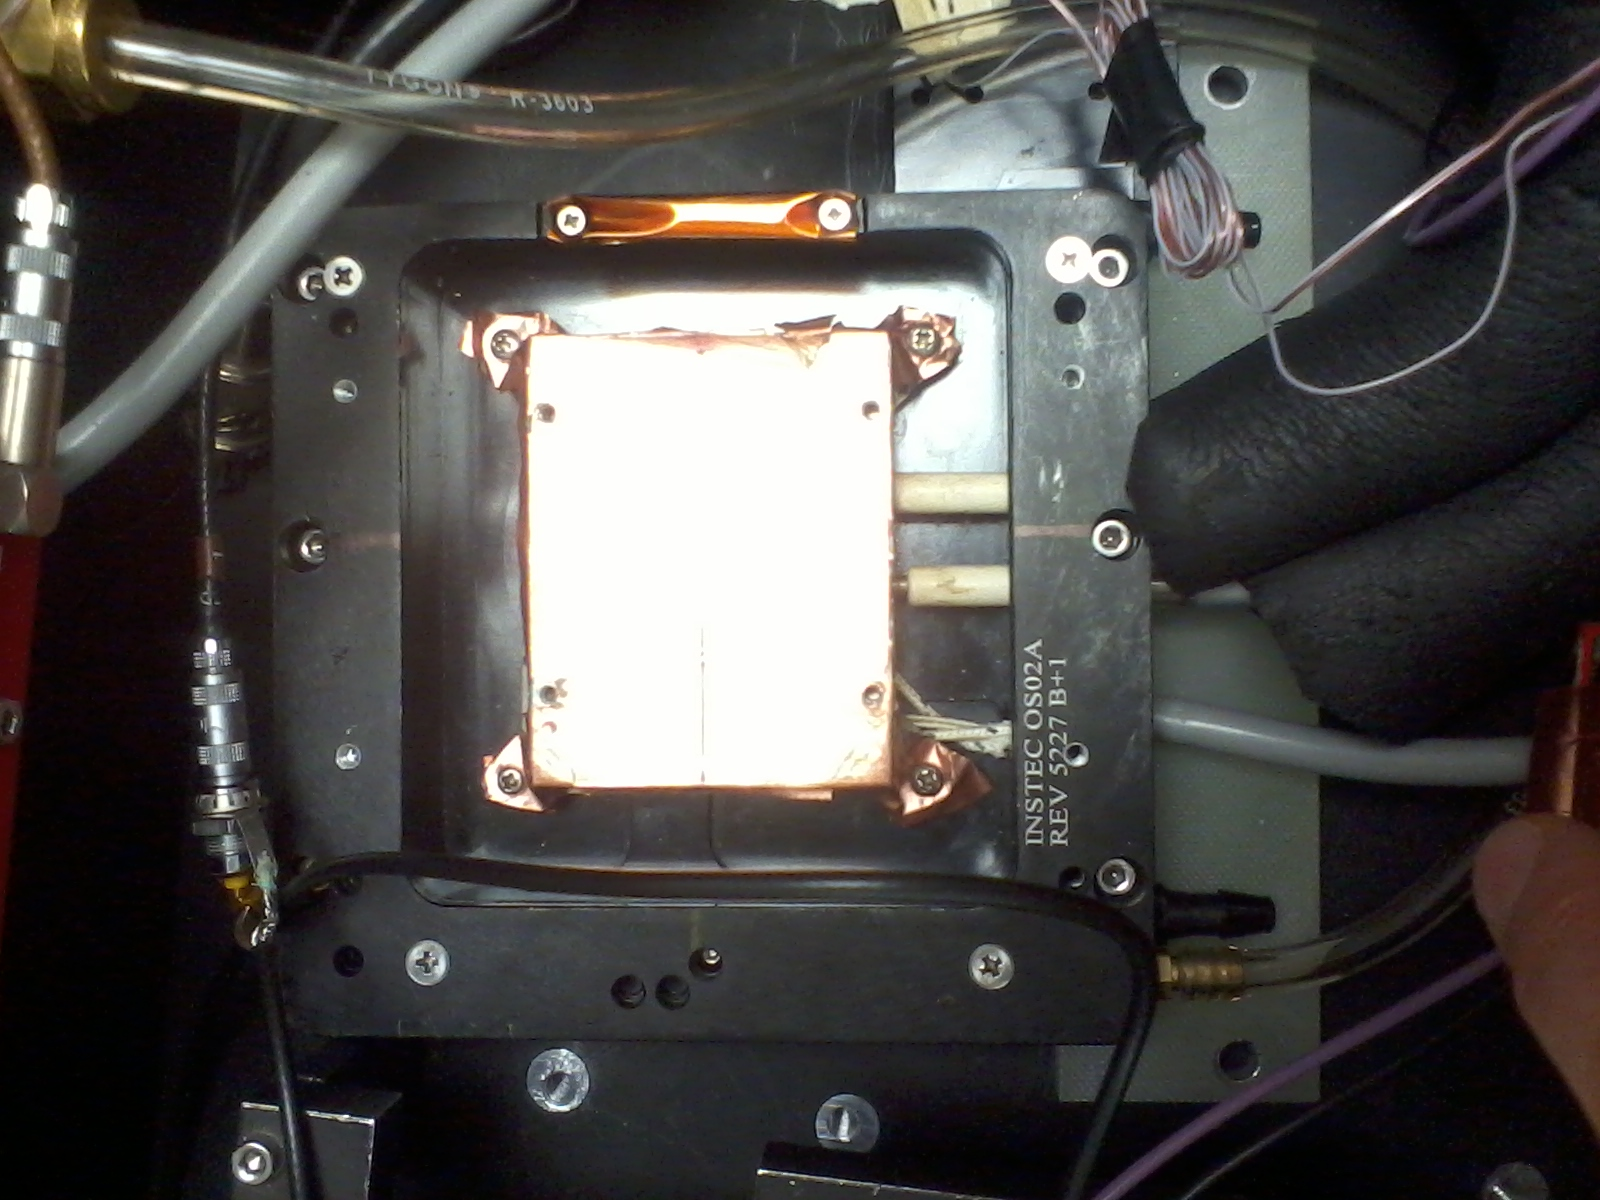
\includegraphics[totalheight=.3\textwidth,trim=5cm 0cm 6cm 0cm, clip=true]{../Pictures/Pictures_Setup/shock.jpg}%trim=10cm 4cm 1cm 12cm, clip=true, 
      \label{fig:cooling_shock}}
    \end{subfigure}
    \quad
    \begin{subfigure}[VUV3 SIPM of HAMMAMATSU centered on the shock.]{%
      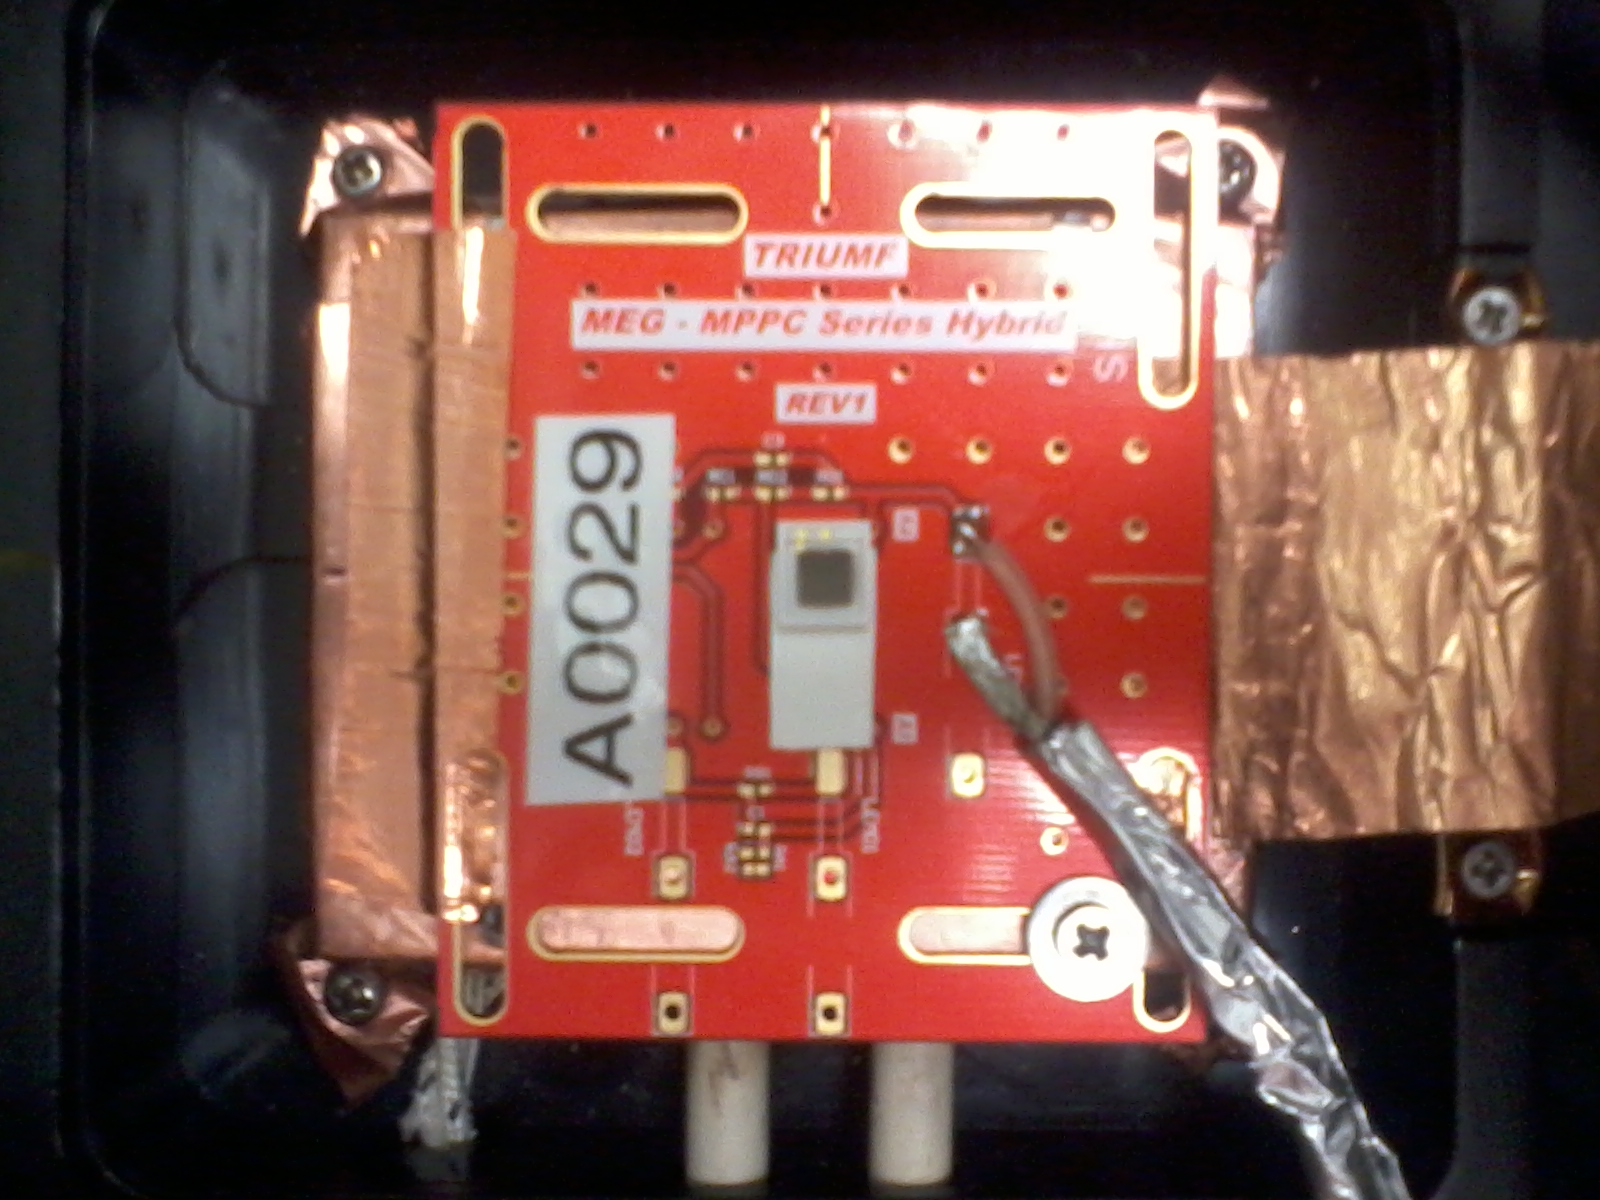
\includegraphics[totalheight=.3\textwidth,trim=0cm 0cm 0cm 0cm, clip=true]{../Pictures/Pictures_Setup/VUV2_on_shock.jpg}
      \label{fig:VUV3}}
    \end{subfigure}
  \caption{A VUV3 SiPM centered on the cooling shock.}
  \label{fig:VUV3_cooling_shock}
  \end{figure}  
  
  Several different SiPMs are tested to select the more suitable one for nEXO.
  
  \begin{figure}[!hbtp]
    \begin{tcolorbox}[tab2,tabularx={X||Y|Y|Y|Y},title=SiPMs from HAMMAMATSU,boxrule=0.5pt]\label{elementary_particle}
	      &Efficiency &Dark Noise rate &Cross Talk & After Pulse \\\hline\hline
      MPPC MEG &no &yes &yes &no  \\\hline
      VUV3 SiPM &no &yes &yes &yes  \\\hline
      Coated SiPM &no &yes &yes &no  \\\hline\hline
    \end{tcolorbox}
  \caption{Differents SiPM from HAMMAMATSU are tested.}
  \label{fig:table_SiPM}
  \end{figure}
  
  
  \subsection{Temperature sensors and automation}
  
  We noticed that the whole box is cooling down over time when we are working at $-100^{\circ}$C. The plastic holder of the figure
  \ref{fig:cooling_shock} doesn't isolate totally the colling shock from the rest the box.\\
  To check if the decreasing temperature of the box could have an impact on our results (efficiency), 10 temperature sensors are 
  installed inside the box after calibrating them \ref{app:tests}. All temperatures of the sensors are recorded automatically.  
  
  \newpage
  
  \begin{figure}[!hbtp]
  \centering
    \begin{subfigure}[One of the ten temperature sensors.]{%
      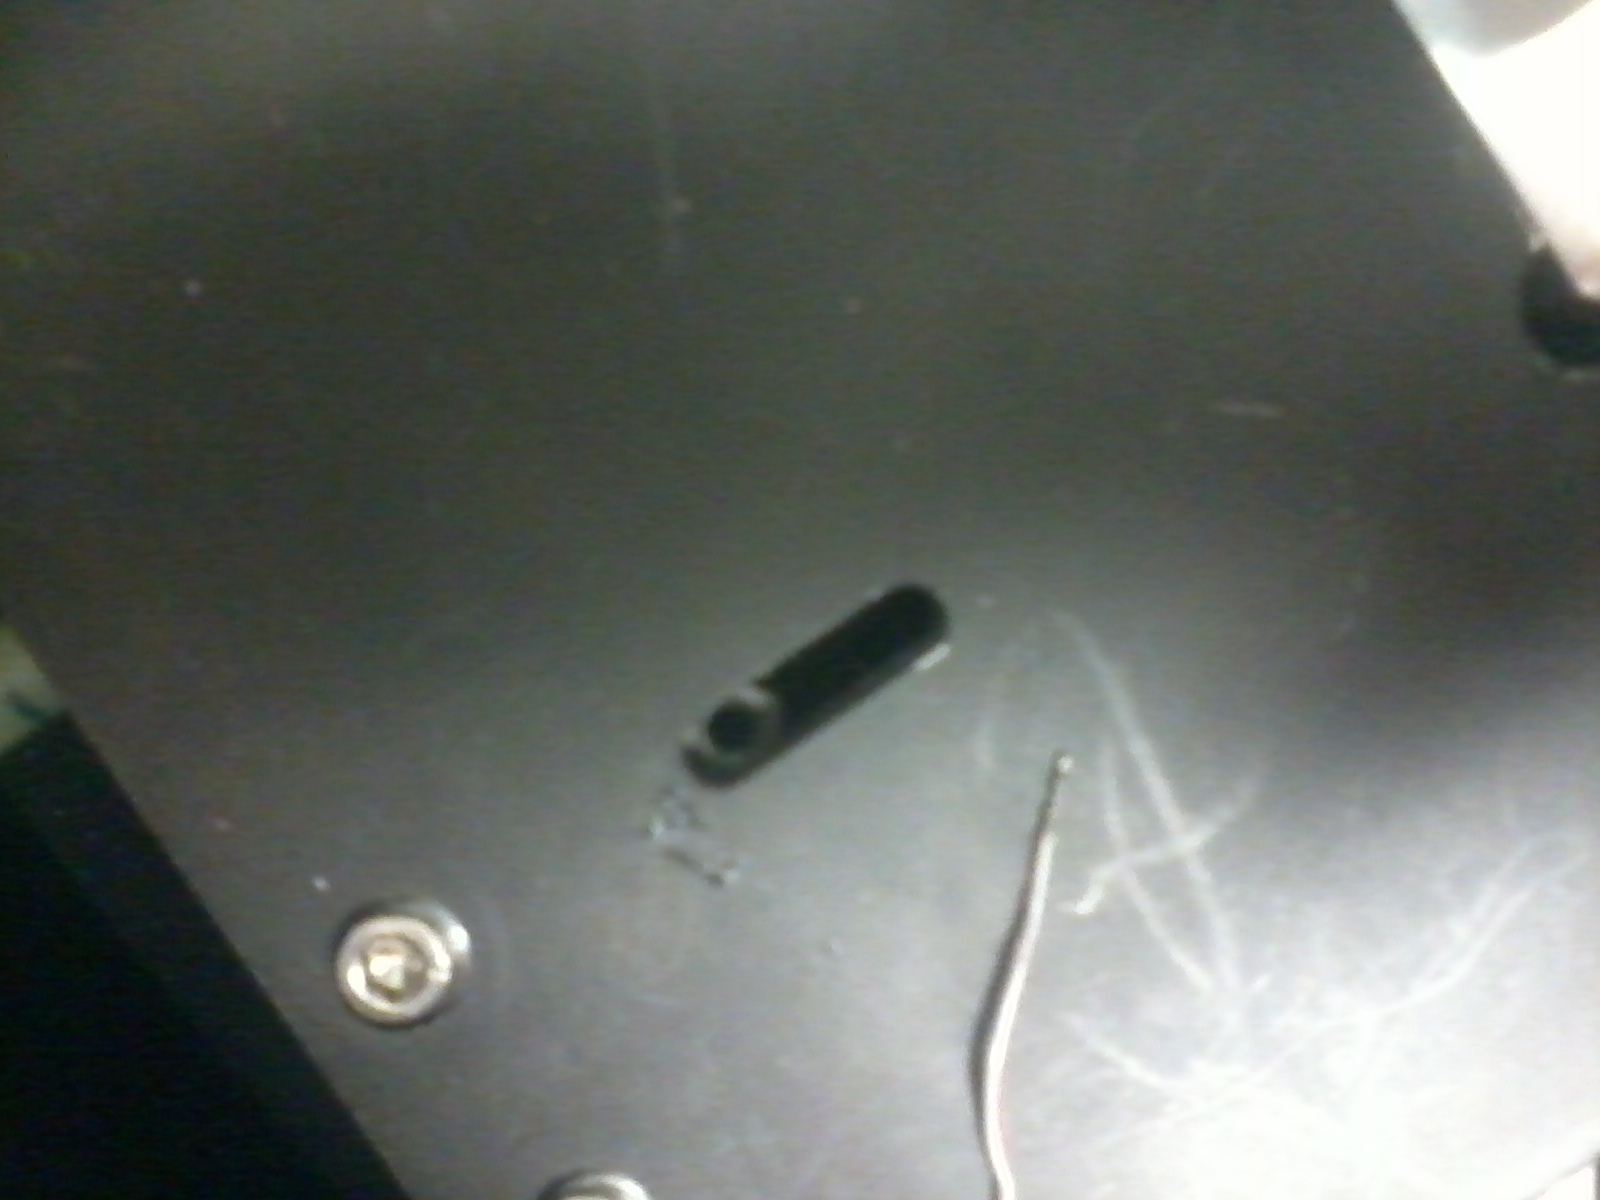
\includegraphics[totalheight=.2\textwidth,trim=0cm 7cm 0cm 2.5cm, clip=true]{../Pictures/Pictures_Setup/temp_sensor.jpg} 
      \label{fig:temp_sensor}}
    \end{subfigure}
  \quad  
    \begin{subfigure}[That device lets record temperatures from sensors.]{%
      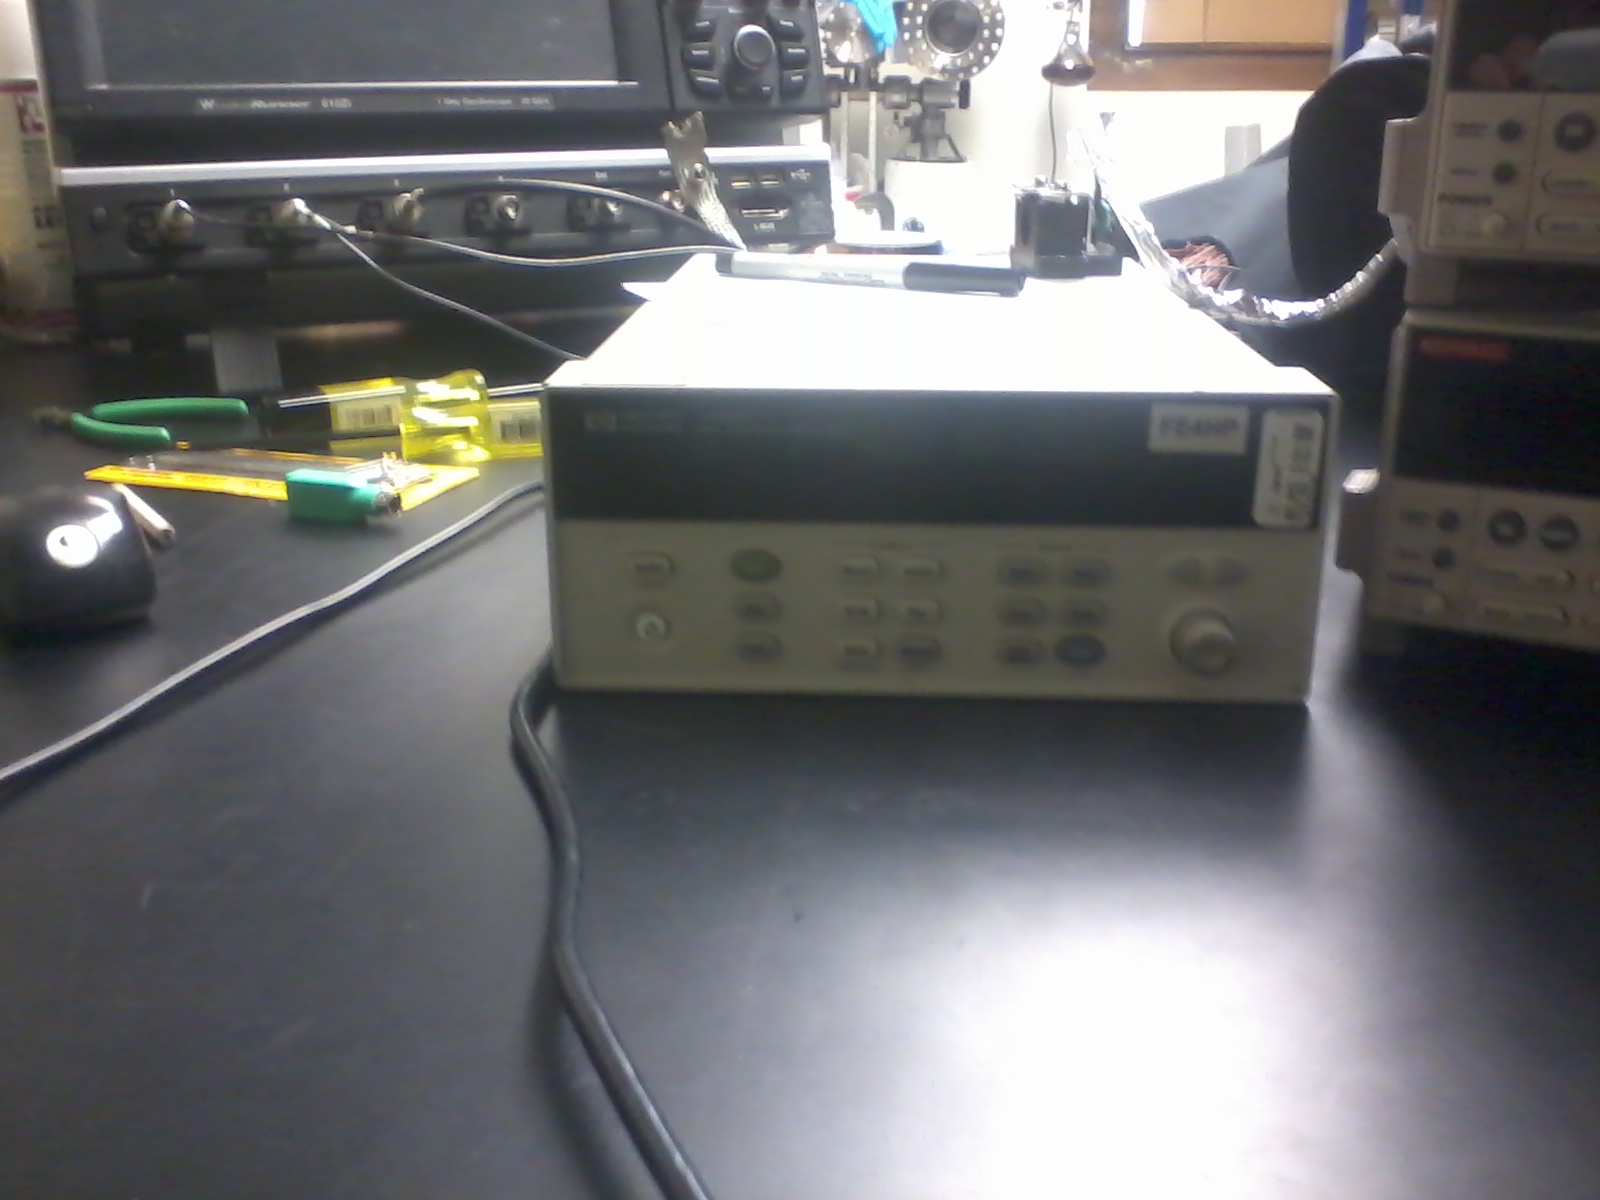
\includegraphics[totalheight=.2\textwidth,trim=18cm 17cm 7cm 10cm, clip=true]{../Pictures/Pictures_Setup/temp_device.jpg}
      \label{fig:temp_device}}
    \end{subfigure}
  \caption{Those devices allow registering temperatures from different parts of the box.}
  \label{fig:temp_sensor_device}
  \end{figure}
  
  Also a program is written to set the voltage, to record both the current of the photo-detectors and temperatures from
  different parts of the box. 
  
  \section{Silicon Photo-Multiplier}
  
  A Silicon photomultiplier (SiPM) is an electronic device used to detect light (photon). Many groups study their applicability 
  in many different 
  fields such as high-energy, physics calorimetry, astrophysics or medical imaging.\\ %\reference ou pas ??
  Compared to EXO experiment which uses currently APD, SiPMs for nEXO experiment are a very promising 
  alternative because of the very good properties of such devices:
  
  \begin{itemize}
   \item SiPMs are incentive to magnetic fields,
   \item SiPMs' operation voltage is very low,
   \item SiPMs' gain is \(10^6 - 10^7\),
   \item SiPMs have a very good time (ns) and photon-counting resolutions ($\Pmu$m) due to the size of one pixel.
  \end{itemize}

  \subsection{Structure}
  
  This device consists a matrix of typically 1000 independent and equal micro-cells (pixels) per mm\texttwosuperior{}. A pixel 
  consists the basic element of SiPMs.\\
  Each pixel are connected in parallel. They are formed out of an Avalanche Photo Diode (APD) and a quenching resistor which is 
  connected in series to an APD. 
  \newpage
  
  \begin{figure}[!hbtp]
  \centering
    \begin{subfigure}[A MPPC SiPM from HAMMAMATSU VUV sensitive.]{%
      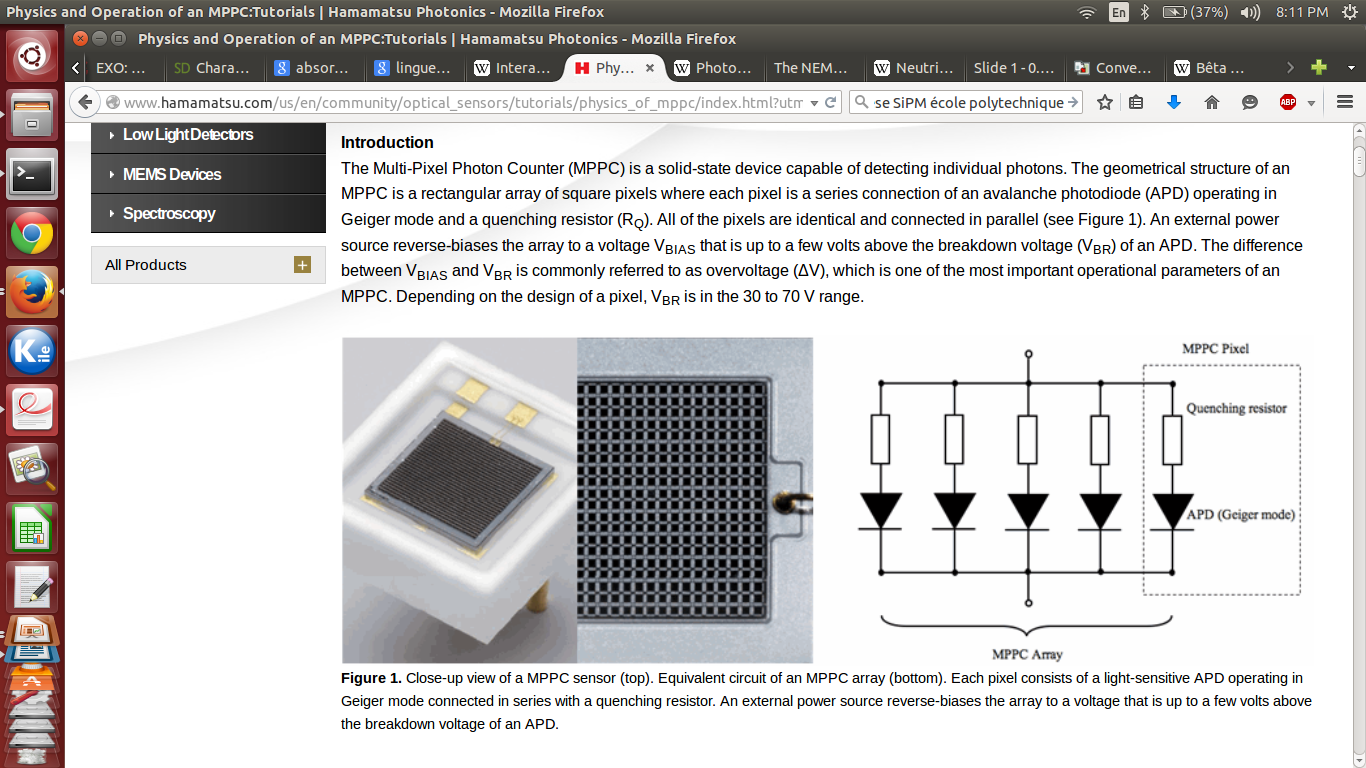
\includegraphics[totalheight=.27\textwidth,trim=12.07cm 4.1cm 19.55cm 12cm, clip=true]{../Pictures/hammamatsu.png} 
      \label{fig:MEG}}
    \end{subfigure}
  \quad  
    \begin{subfigure}[Equivalent circuit.]{%
      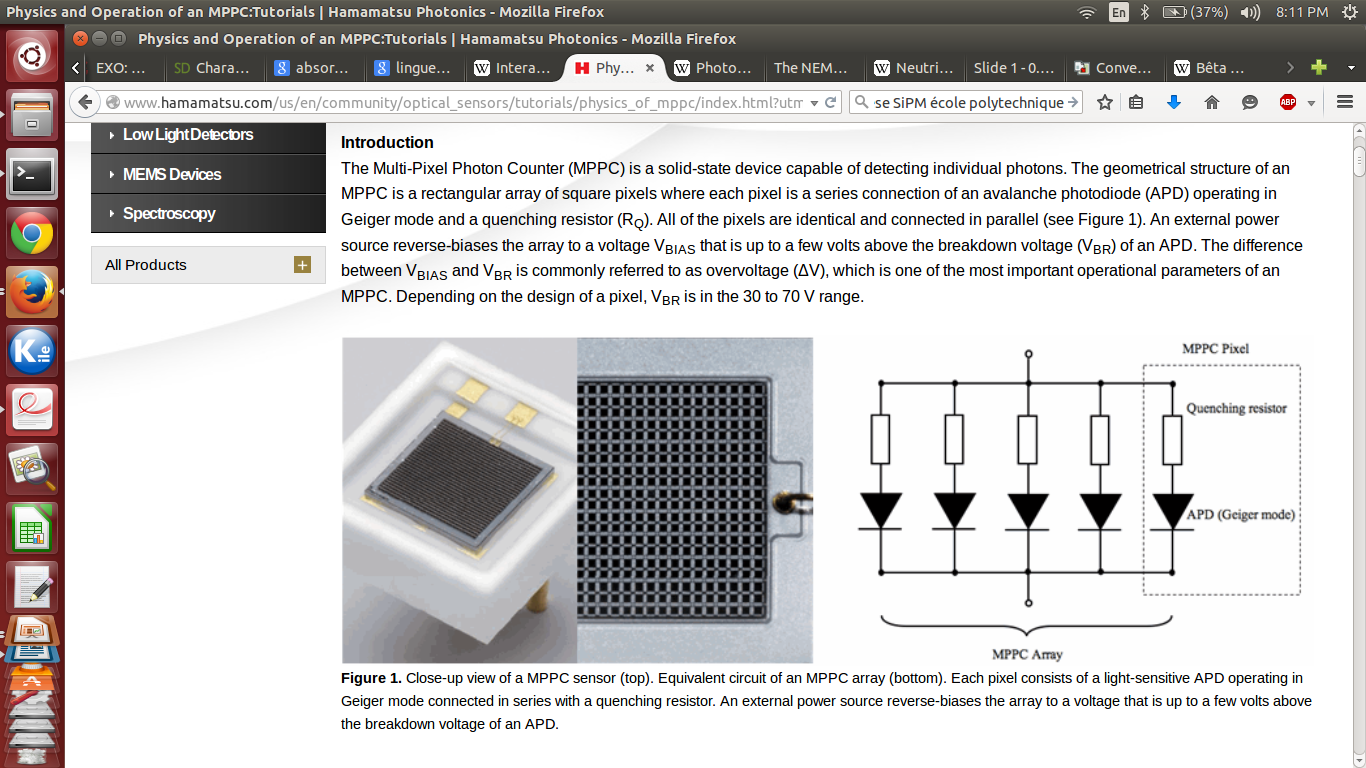
\includegraphics[totalheight=.27\textwidth,trim=30cm 3.6cm 1cm 12cm, clip=true]{../Pictures/hammamatsu.png}
      \label{fig:electrical_circuit}}
    \end{subfigure}
  \caption{Documentation about SiPM is provided by HAMMAMASTU \cite{ref:mppc_hammamatsu}.}
  \label{fig:temp_sensor_device}
  \end{figure}
  
  The appendix \ref{app:setup} gives more details about the amplification of signals from photo-detectors. 
  
  \subsection{Basic operation}\label{subsec:basic_operation}
  
  Each pixel in a SiPM outputs a pulse at the same amplitude when it detects a photon. 
  A pulse produced from one pixel doesn't vary with the number of incident photons firing that pixel. 
  All pixels are connected to the same output channel. The total output signal is equal to the sum of those from the individual pixels 
  firing by photons.
  \\
  
  For example, if four photons are incident on different pixels and detected at the same time, then the SiPM outputs a signal whose 
  amplitude equals the height of the four superimposed pulses.

  %So the number of output pulses is always one regardless the number of incoming photon. This means that MPPC output linearity gets worse 
  %as more photons are incident on the MPPC such as when two or more photons enter one pixel. This makes it essential to select an MPPC 
  %having enough pixels to match the number of incident photons.
 
  One feature of an SiPM is that each APDs operate in Geiger mode.
  
  \subsection{Physical APD's operation}

  \subsubsection{\textit{\underline{PN Junction}}}
  
  A pixel is a photo-diode and a photo-diode has the structure of a PN junction. This reference \cite{ref:PN_junction_ref} could remind the reader how 
  a PN junction works:
  
  \newpage
  
  \begin{figure}[!hbtp]
  \centering
    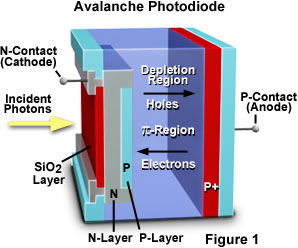
\includegraphics[trim=0cm 0cm 0cm 0cm, clip=true,totalheight=.4\textwidth]{../Pictures/APD_Hammamatsu.jpg} 
    \caption{A photo-diode shown as a PN junction \cite{ref:Hammamatsu_pn_junction}.}
    \label{fig:PN_junction}
  \end{figure}
    
  \subsubsection{\textit{\underline{Principe of avalanche multiplication}}}
  
  The principle of an APD is based on the conversion of the energy of photon into free charge carriers (electrons and 
  holes) in the depletion region
  and their further multiplication via the process of the impact ionization. 
  \\
  When light (photon) enters a photo-diode, electron-hole pairs are generated if 
  the light energy is higher than the band gap energy. Light energy - $E_{light}$ in electron-volt (ev)- and wavelength $\lambda$ (nm)
  are in relationship as shown in equation (number) below. 
  
  \begin{equation}
   E_{light} = \frac{123}{\lambda}
  \end{equation}
  
  A reverse voltage (or bias voltage) is applied to each opposite sides (cathode and anode) of a PN junction. 
  The reverse voltage applied on an PN junction is upper than the Breakdown Voltage (BV) of that 
  APD: this is the Geiger mode \footnote{Conventional photo-diodes operate in linear mode}.  
  
%   \begin{figure}[!hbtp]
%   \centering
%     \begin{subfigure}[Different modes available for a photo-diode. All tension applied on the SiPMs is 
%     below their own breakdown voltage $V_{breakdown}$. $V_{breakdown}$ increase when the temperature decrease.]{%
%       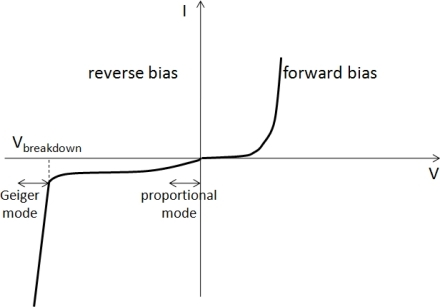
\includegraphics[totalheight=.3\textwidth,trim=0cm 0cm 0cm 0cm, clip=true]{../Pictures/geiger.png}
%       \label{fig:geiger}}
%     \end{subfigure}
%   \quad  
%     \begin{subfigure}[The gain becomes infinite when the photo-diode is set in  the Geiger mode.]{%
%       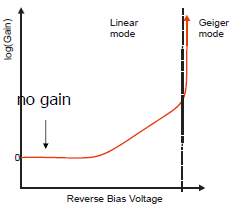
\includegraphics[totalheight=.3\textwidth,trim=0cm 0cm 0cm 0cm, clip=true]{../Pictures/geiger_gain.png}
%       \label{fig:electrical_circuit}}
%     \end{subfigure}
%   \caption{SiPM was working in the Geiger mode.}
%   \label{fig:geiger_gain}
%   \end{figure}
  
  The reversed (or biased) voltage $V_{biased}$ and the breakdown voltage $V_{breakdown}$ are linked with the over-voltage (OV or $\Delta V$) according to that relation :
  
  \begin{equation}
    \Delta V = V_{biased} - V_{breakdown}
  \end{equation}

  Also this reverse voltage creates an electric field developed across the PN junction.\\
  When an electron-hole pair is generated in the depletion layer of a photo-diode 
  the electrons (negative charge) drift towards the N layer (where the cathode is) while the holes drift towards the P+ layer 
  (where the anode stays). This migration is due to the electric field. 
  \\
  
  The drift speed of these electron-hole pairs or carriers depends on the electric field strength. To a certain speed
  the carriers collide with the atoms (called crystal lattice) of the structure. If the reverse voltage is increasing even further, 
  some of the carriers which escaped primary collision with the crystal lattice will have a great energy.\\
  When they collide later with the crystal lattice, they will generate other electron-hole pairs. This physical phenomena is called 
  ionization:
  an electron or a hole with high kinetic energy ionizes the matter by triggering other electron-hole pairs. 
  By the end an avalanche phenomena is observed inside the avalanche region of a PN junction:
  
  \begin{figure}[!hbtp] 
  \centering
    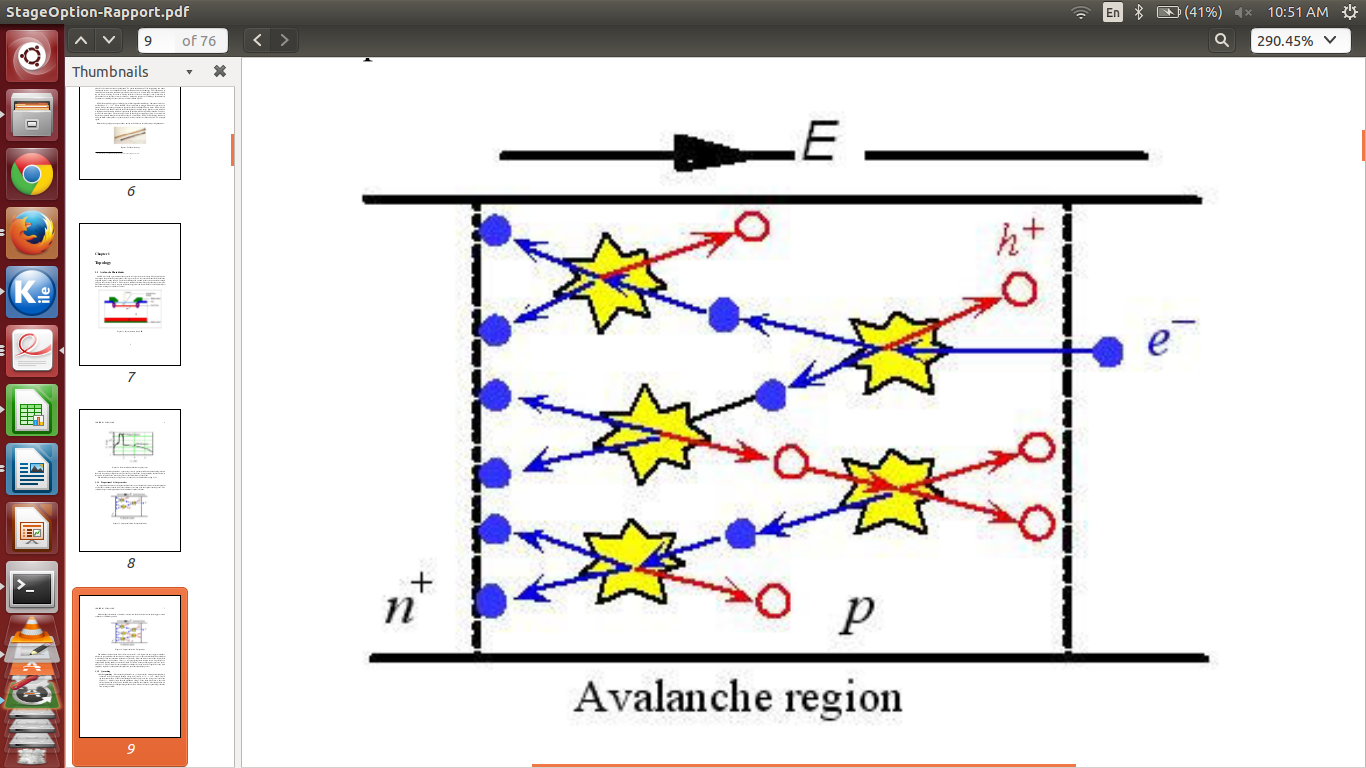
\includegraphics[totalheight=.35\textwidth,trim=12.8cm 1.5cm 5.5cm 4cm, clip=true,]{../Pictures/avalanche.png}
    \caption{A photon triggers an avalanche of electron-hole pairs inside the PN junction.}
    \label{fig:avalanche}
  \end{figure}
  
  The electrons of that avalanche phenomena are collected on the cathode. The resulting current is used to plot the  pulse shape. 
  To control an avalanche and so the corresponding current, a resistor is set in series with an PN junction \footnote{The avalanche 
  is also limited by the buildup of a limiting space charge in the depletion region which makes decrease the field.}. 
  When the avalanche current flows through the resistor, the bias voltage applied to the junction drops below the breakdown voltage. 
  This quenches the avalanche; thus, the current decreases to zero, and the reverse voltage across the PN junction increases again above 
  its BV.\\
  Then the pixel is ready to detect the arrival of a new photon.
  \\
  
  A single pixel avalanche gives a pulse shape observed on the screen of an oscilloscope: 
  
  \begin{figure}[!hbtp] 
  \centering
    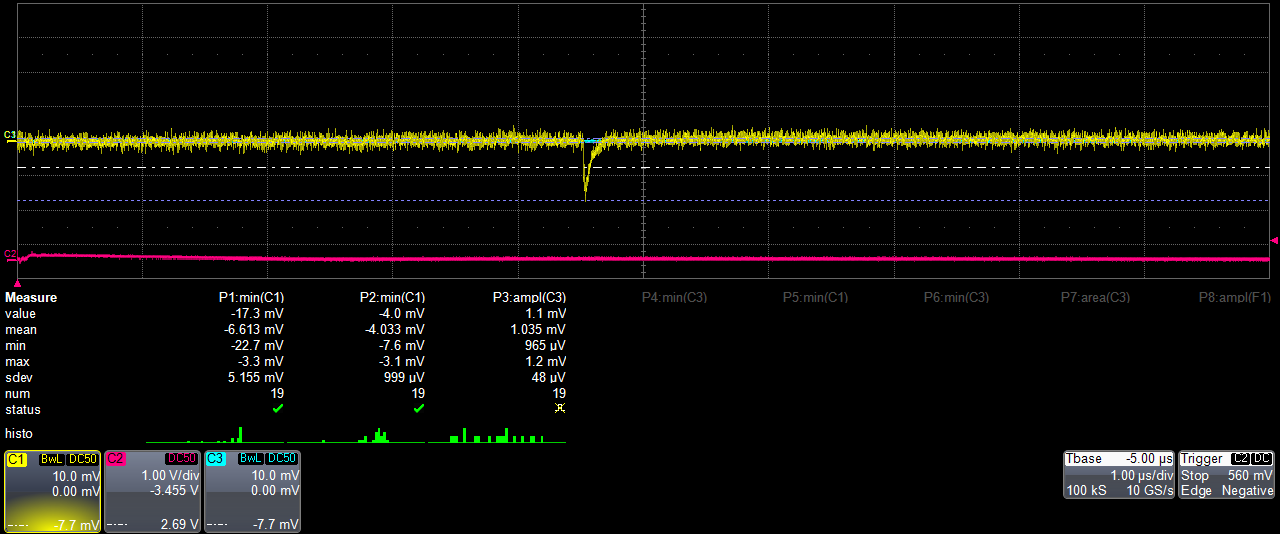
\includegraphics[totalheight=.2\textwidth,trim=0.3cm 6.6cm 0.1cm 0cm, clip=true,]{../Pictures/blabla/pulse_shape.png}
    \caption{One pixel of the VUV3 SiPM is firred by photons. Here is the corresponding single pixel avalanche which
    gives such a pulse shape. Horizontal axis is the time (1$\Pmu$s/div) and Vertical axis is the voltage measured from the photo-detector (10mv/div).}
    \label{fig:avalanche}
  \end{figure}
  
  %about the gain, simple approximation speak about it ???? not now but in the gain stuff inside the corpus if room therwise in the 
  %appendix
  %Gain: The gain of the SiPM determines the charge which is produced by a single avalanche.
  %In good approximation, the gain depends linearly on the pixel capacitance C pixel and the
  %applied over-voltage V over which is defined as the difference of the bias voltage and the
  %breakdown voltage:
  %C pixel
  %C pixel
  %G = ·V over =   · (V bias −V break ).  (2.1)  q e  q e
  %Here, q e is the elementary charge and C pixel the pixel capacitance.
  
  \newpage
  
  \subsection{The three main issues of an operating SiPM} 
  
  Such an ideal picture is strongly modified by the occurrence of phenomena leading to dark current, after-pulsing effects and crosstalk: 
  
  \begin{figure}[!hbtp]
  \centering
    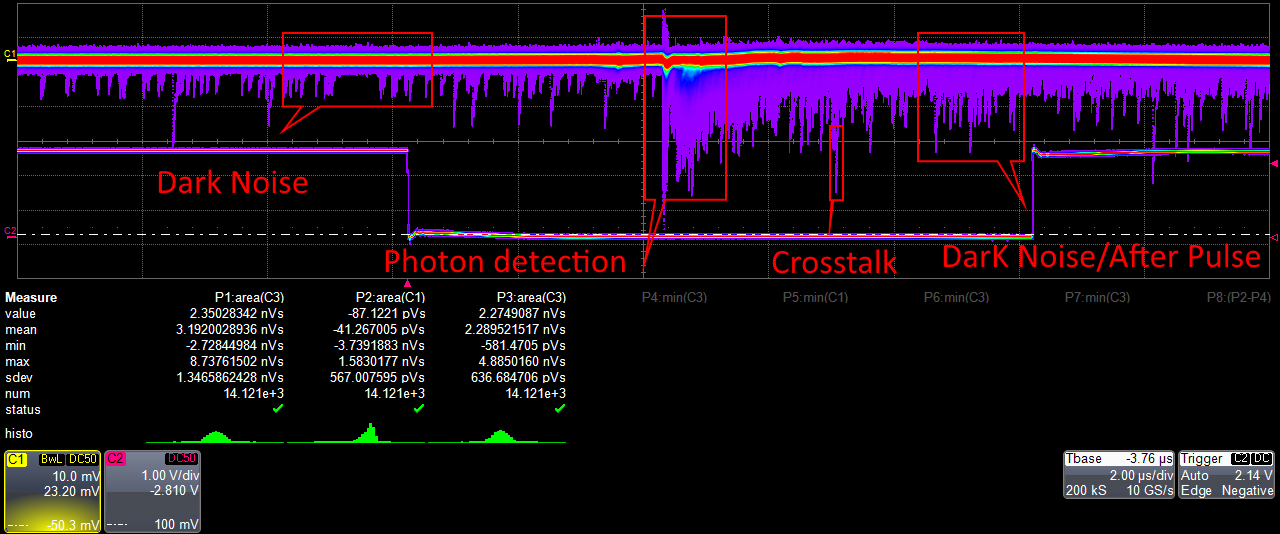
\includegraphics[totalheight=0.2\textwidth,trim=0.3cm 6.6cm 0.1cm 0cm, clip=true]{../Pictures/Pictures_oscilloscope/DN_AP_CT_1.jpg}
    \caption{Dark noise, after-pulse and crosstalk.Horizontal axis is 1$\Pmu$s/div and Vertical axis is 10mv/div.}
    \label{fig:DN_AP_CT}
  \end{figure}
  
  \subsubsection{\textit{\underline{Dark Noise}}}\label{subsubsec:DN_photon_shape}
  
  One of the main source of noise limiting APDs' performance is the dark noise rate.\\
  Electron-hole pairs are generated thermally in the depletion region. Due the reversed bias voltage applied on the PN junction, 
  the avalanche phenomena occurs.
  Unfortunately it is not possible to make the difference between avalanche triggered by a photon and avalanche triggered by hot carriers.
  The figure below shows that evidence:
  
  \begin{figure}[!hbtp]
  \centering
    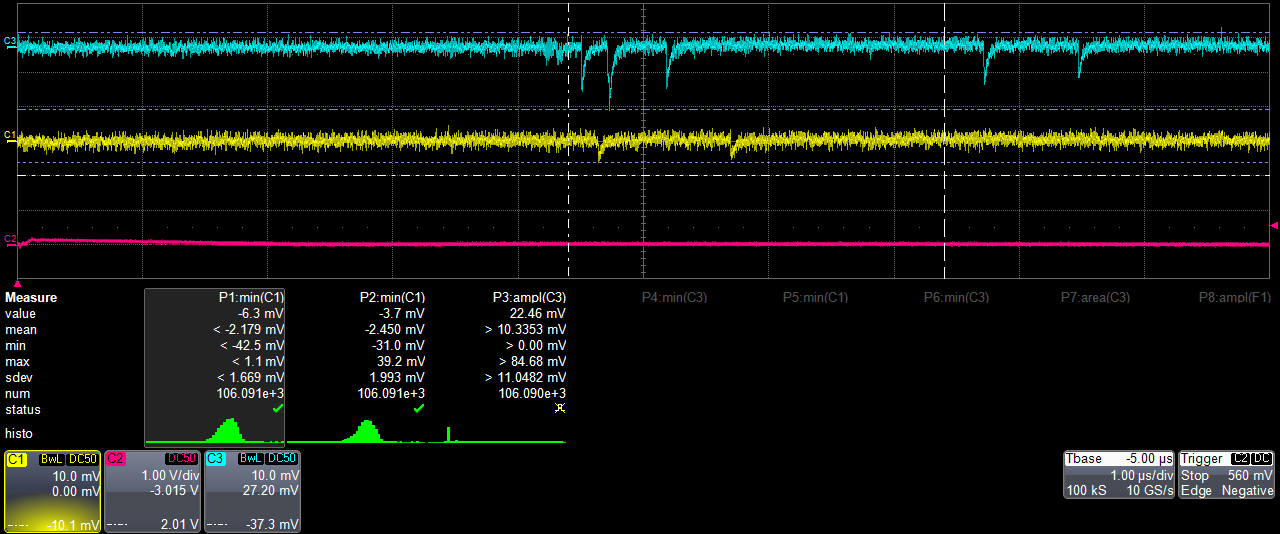
\includegraphics[totalheight=0.2\textwidth,trim=0.3cm 6.6cm 0.1cm 0cm, clip=true]{../Pictures/Pictures_oscilloscope/DN_photon.png}
    \caption{Pulse shapes from a pixel firred by an incoming photon (centered) are exactly the same than pulse shape triggered by hot carriers (left).
    The blue signal comes from the detector on the top while the yellow one comes from the detector on the bottom.
    Horizontal axis is 1$\Pmu$s/div and Vertical axis is 20mv/div.}
    \label{fig:DN_photon}
  \end{figure}
  
  Dark noise depends only of the structure of the SiPM. VUV3 SiPM from HAMMAMASTU has a lower dark noise rate than VUV2 or MPPC MEG 
  from the same manufacturer.
  Nevertheless it is possible to decrease the dark noise rate by cooling down the SiPM since dark noise is generated by 
  hot carriers.  
  \\
  \\
  
  Crosstalk and after-pulses are generated by primary peaks. By definition a primary peak can be triggered by photon or by hot carriers. 
  
  \subsubsection{\textit{\underline{Trapping phenomena: Afterpulsing}}}\label{subsubsec:AP_section}

  Traps may result from damage caused by an implantation of some impurities in the fabrication process. In the depletion region, 
  deep levels trap some avalanche carriers and release them with 
  a statistical delay. If the delay is greater than the dead time after the previous avalanche pulse, a released carrier can
  re-trigger an avalanche and cause a statistically correlated pulse. These delayed correlated pulses are known as after pulses. 
  
  \begin{figure}[!hbtp]
  \centering
    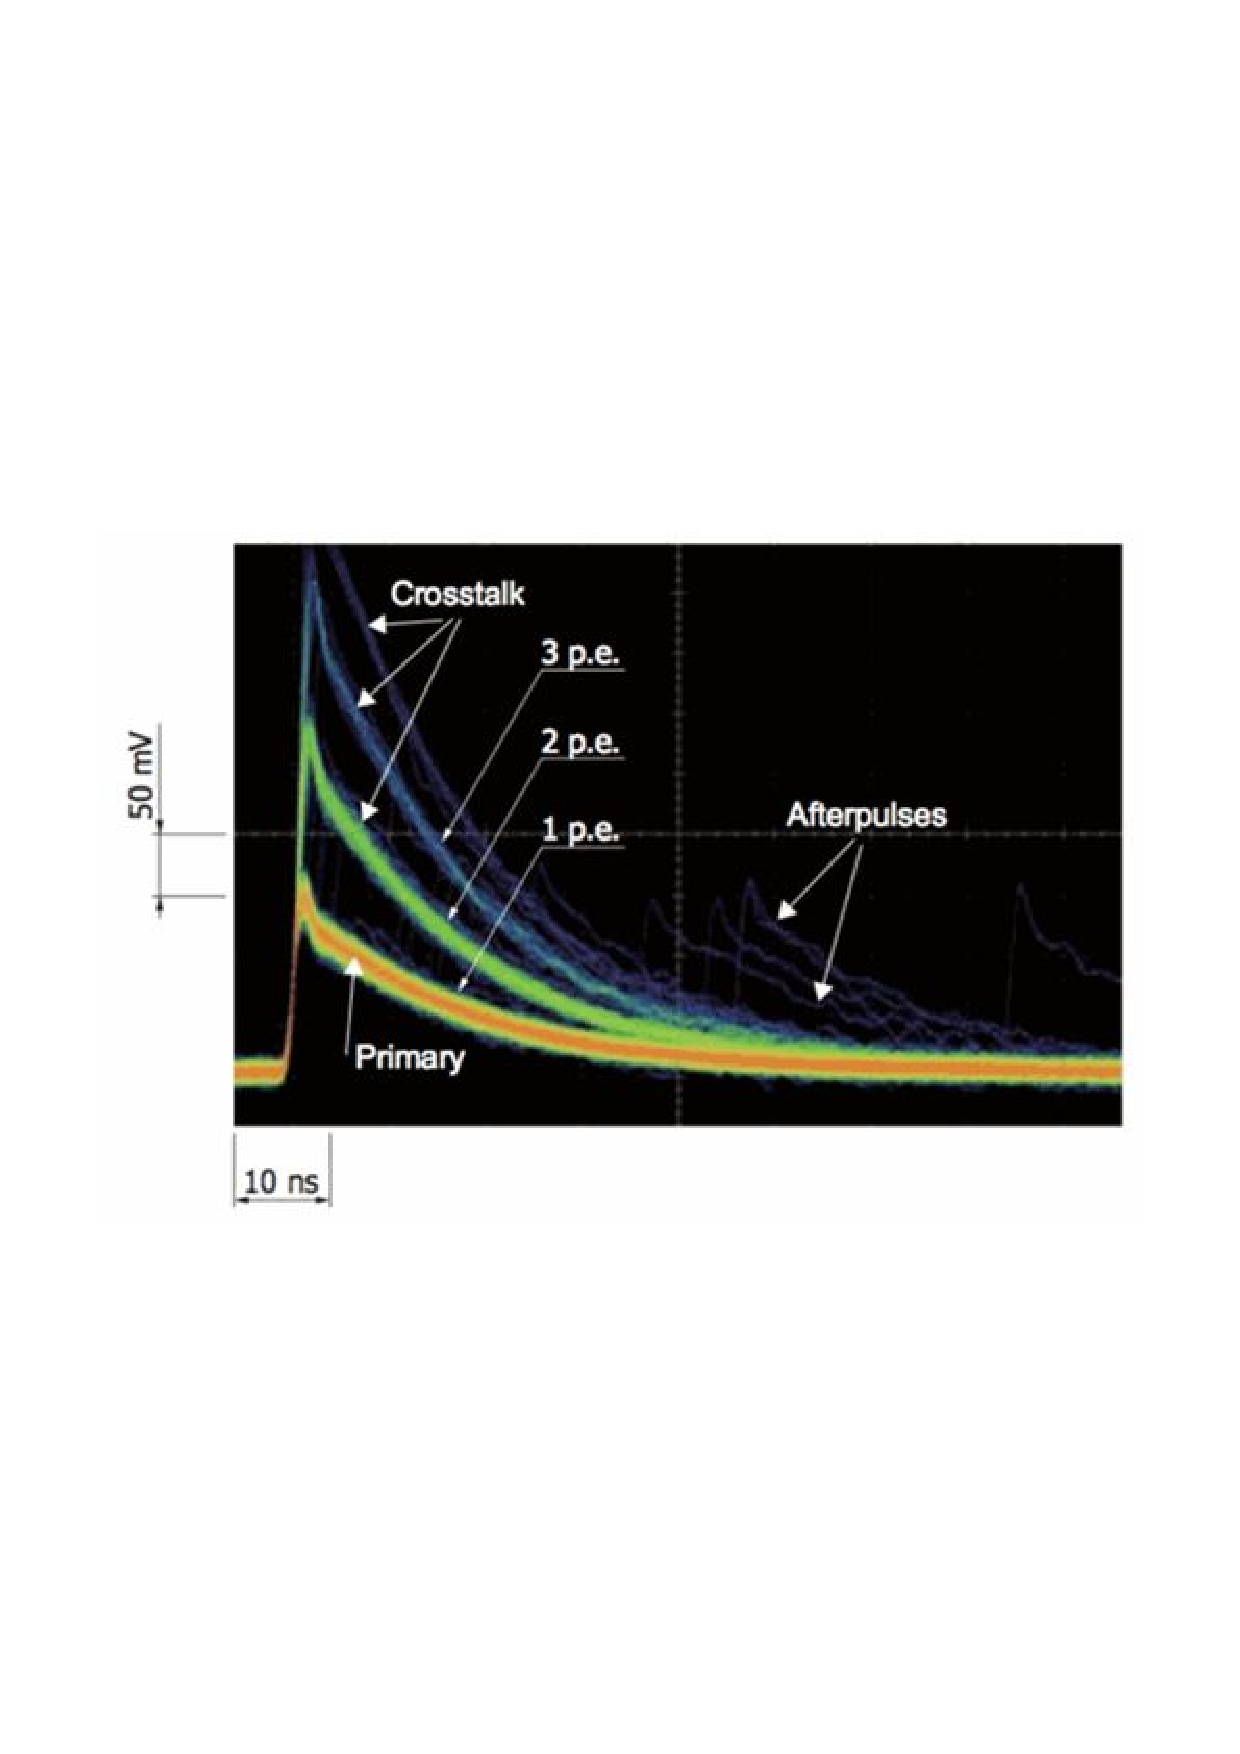
\includegraphics[totalheight=0.5\textwidth,trim=2cm 9cm 3cm 9cm, clip=true, angle = 0]{../Pictures/primary_peak_CT_AP-1.pdf}
    \caption{After pulses are clearly identified with the persistent mode of the oscilloscope \cite{ref:mppc_meg}.}
    \label{fig:AP}
  \end{figure}
  
  The probability that an after pulse occurs increases with the reversed bias voltage applied on the SIPM.  A solution to diminish 
  significantly after pulses effects is 
  to operate at low reversed bias voltage, but at the expense of degrading the photon-detection efficiency \ref{sec:PE}. 
    
  %After pulse follow a law. 
  
  \subsubsection{\textit{\underline{Optical crosstalk}}}\label{subsubsec:CT_section}
  
  In the P+ layer of a PN junction, hot carriers (e.g., dark noise) of an avalanche has a certain probability to emit photons with energy higher than 1.14 ev (higher than 
  the band gap energy of the silicium (1.12ev)).\\
  Depending on their energy and the location where they are produced, these photons have a certain probability to reach a 
  neighboring pixel and to produce an additional avalanche. 
  
  \newpage
  
  \begin{figure}[!hbtp]
  \centering
    \frame{\includegraphics[totalheight=0.22\textwidth,trim=12.3cm 12cm 0cm 3.95cm, clip=true,page = 14]{../MotivationAndIntroduction.pdf}}
    \caption{The incoming \textcolor{red}{photon} triggers hot carriers.Then emitted \textcolor{blue}{photons} may reach a 
    neighboring pixel and trigger there an avalanche \cite{ref:motivation_and_introduction}.}
    \label{fig:CT}
  \end{figure}
  
  When several pixels are fired  by an incoming photons or by photons created in the P+ layer, the high of the resulting pulse shape 
  ``is multiplied'' by the number of fired pixels \footnote{The section \ref{subsec:basic_operation} reminds that ``The total output signal is equal to the sum of those from the individual 
  pixels firing by photons''.}. 
  
  A technical solution is to build an optical wall between two pixels not to let created photons reaching neighboring pixels. The same conclusion about the efficiency for after-pulses can 
  be made for crosstalk.
  \\
  
    
  \section{Encountered issues}  
  
  Before recording waveforms and analyzing them I encountered with some issues but mainly with electronic noise.\\
  Light leaks appeared when the \xfl is operating. They can hinder and negate the results of data collection. 
  Two kinds of light leaks have been observed :
  
  \begin{itemize}
   \item Visible light leaks.
   \item Radiofrequency light leaks.   
  \end{itemize}
  
  \subsection{Visible light leaks}
  
  Visible light leaks come from outside of the box or from the \xfl (visible light leak).\\
  This phenomena has mainly an impact on the dark noise rate and on the calculation of the efficiency.
  To avoid visible light from the \xfl, the lamp is covered with a black box. Also to absorb photons from such visible light
  walls and lid are covered by matt black absorbing vin.\\
  To avoid light from outside of the box, the whole box was covered with a black tissue. The section \ref{app:tests} shows how we checked if 
  some visible light from outside could reach detectors inside the box. 
  
  \newpage 
  
  \begin{figure}[!hbtp]
  \centering
    \begin{subfigure}[A black tissue lets avoid light from outside the box.]{%
      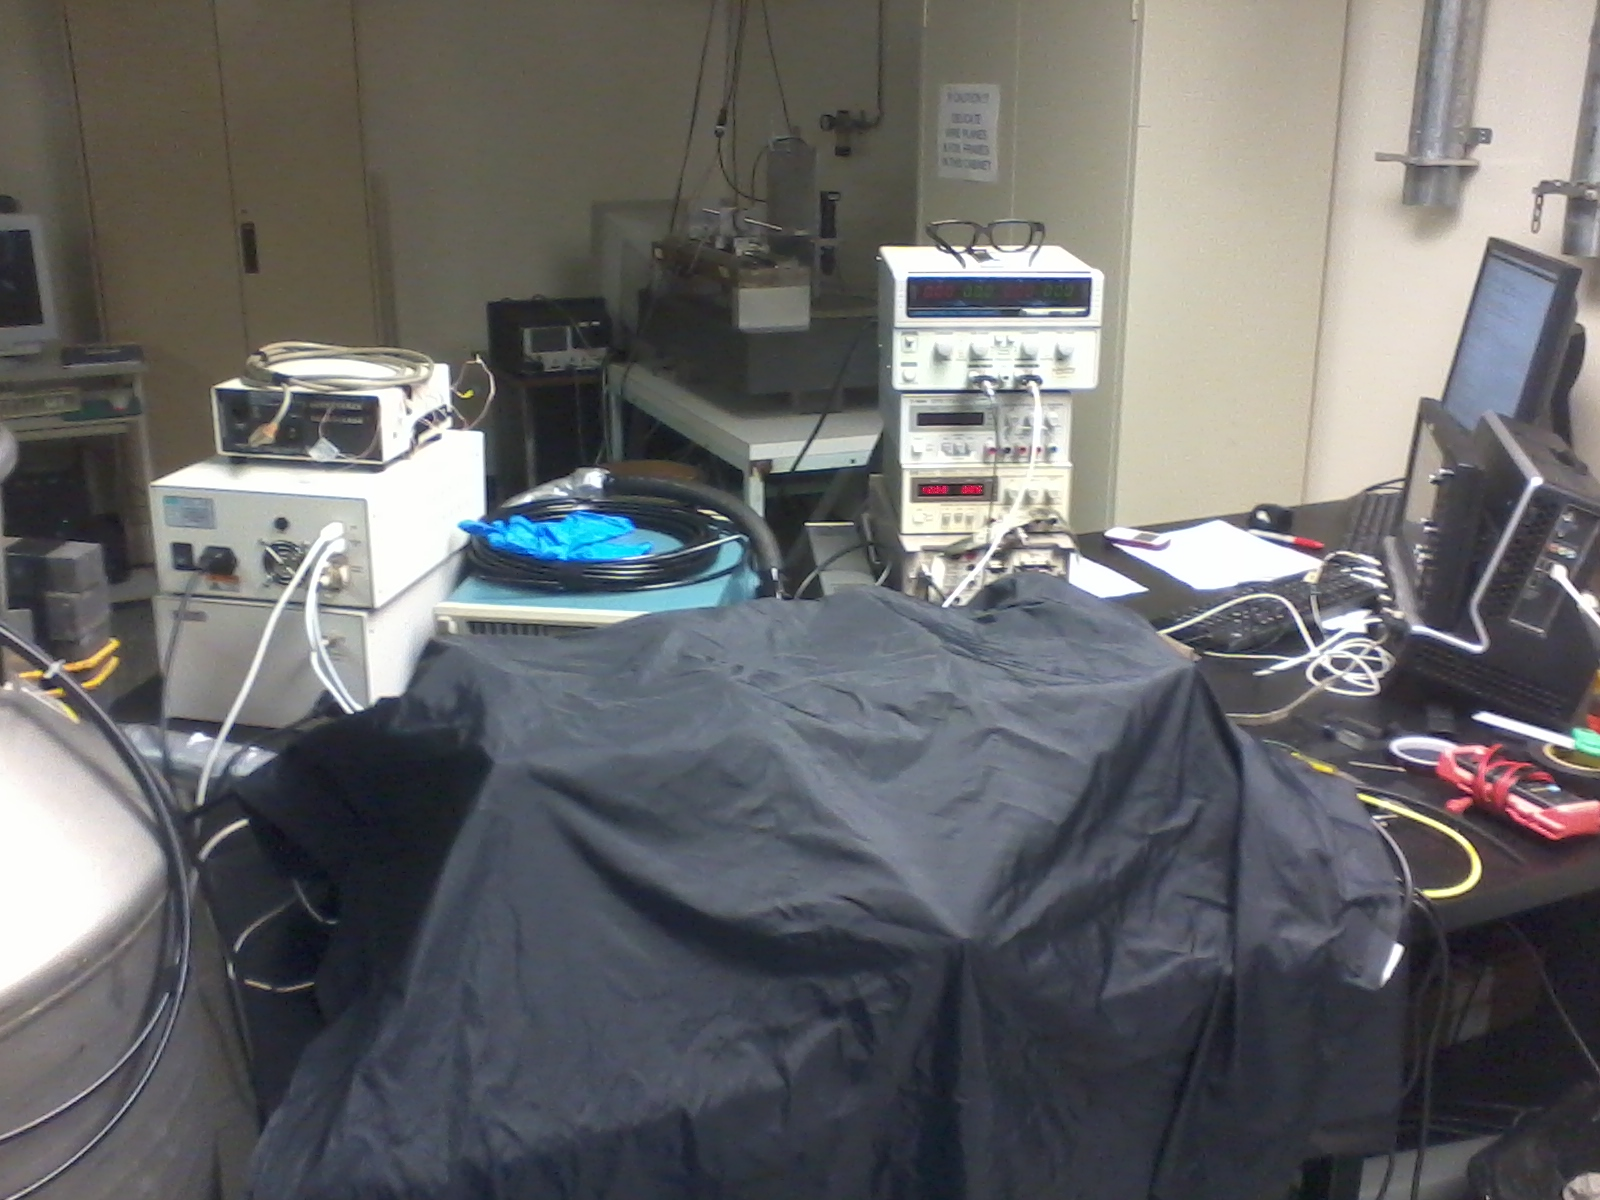
\includegraphics[totalheight=.31\textwidth,trim=0cm 0cm 0cm 0cm, clip=true,]{../Pictures/Pictures_Setup/black_tissue.jpg} 
      \label{fig:black_tissue}}
    \end{subfigure}
  \quad  
    \begin{subfigure}[Black vin, covering the wall and the bottom of the box, absorbs light leaks from the \xfl.]{%
      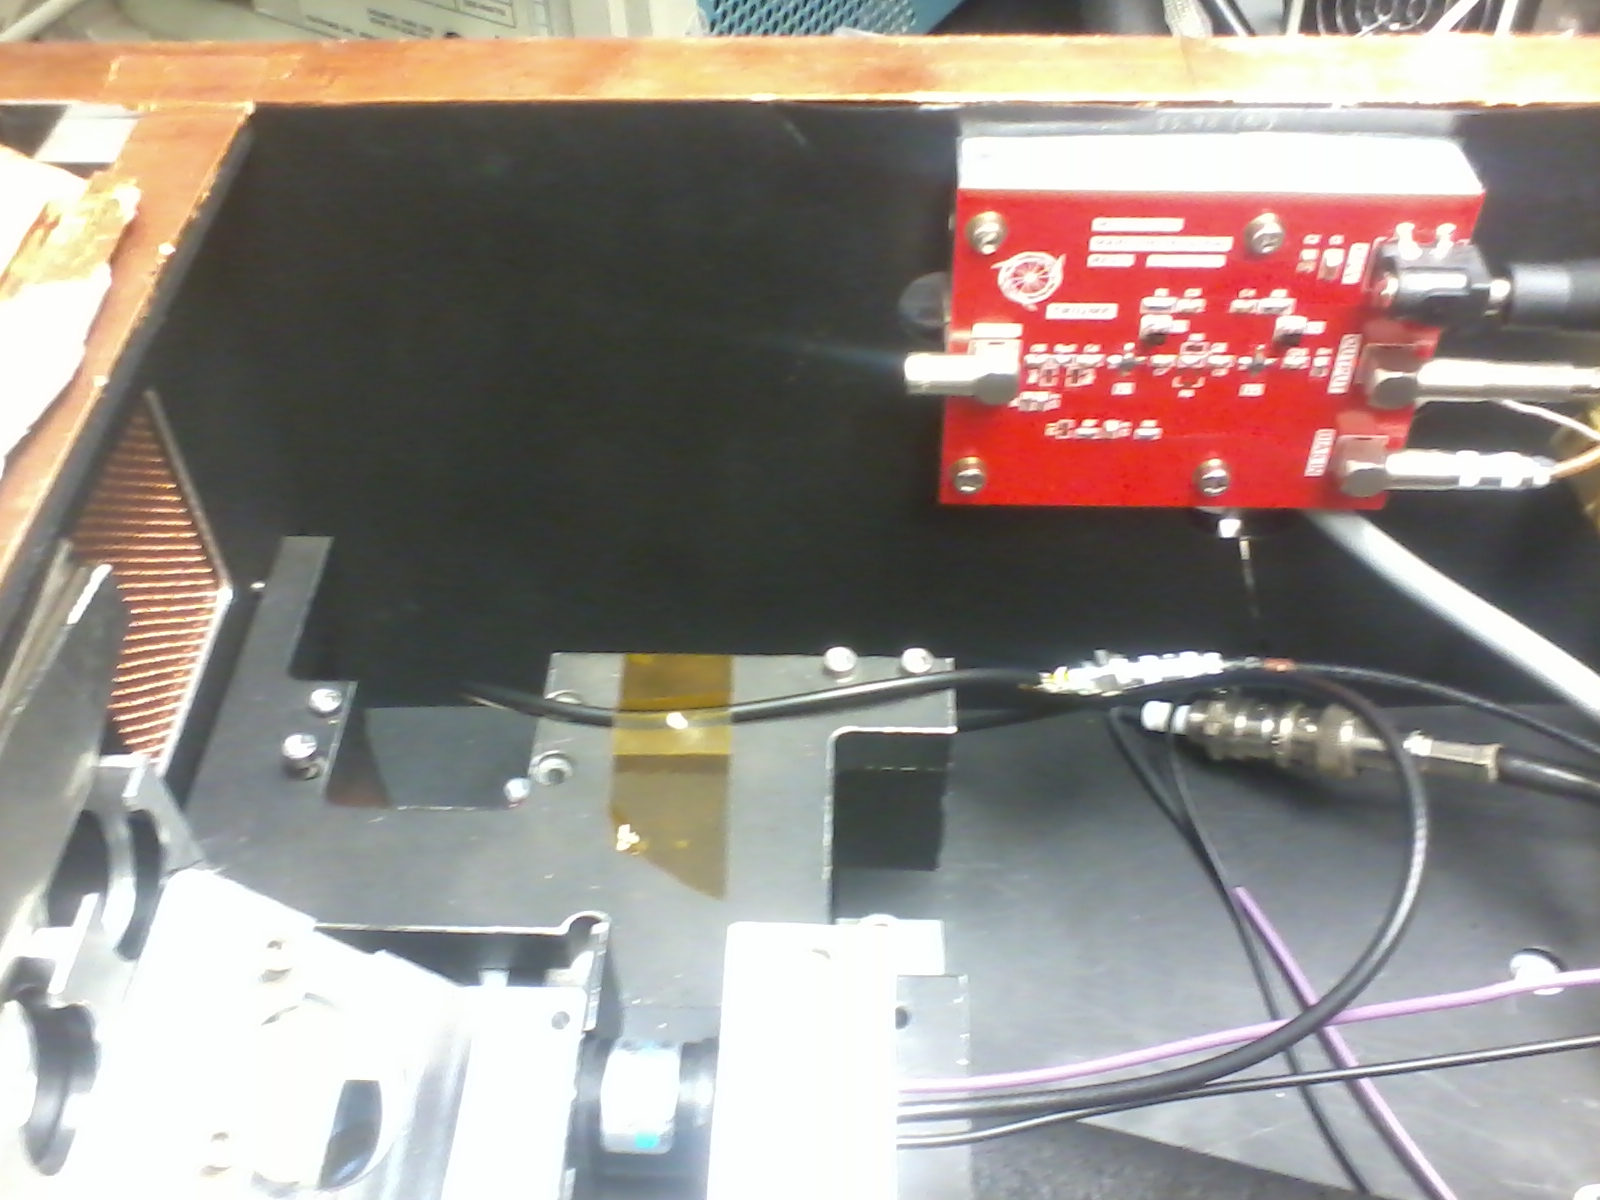
\includegraphics[totalheight=.31\textwidth,trim=0cm 0cm 0cm 0cm, clip=true,]{../Pictures/Pictures_Setup/black_paper_2.jpg}
      \label{fig:black_paper}}
    \end{subfigure}
  \caption{Different solutions to avoid light leaks.}
  \label{fig:black_tissue_paper}
  \end{figure}
  
  \subsection{Radiofrequency light leaks}
  
  Radio frequency light leaks result in electromagnetic noise on the signals from the detectors.\\  
  Radiof frequency noise occurred when the \xfl is triggered (by a square wave pulse generator). Too much radio frequency noise 
  disturbs the signals of the photo-detectors. This figure below shows clearly that electronic noise covers, deforms or amplifies pulse shapes.
  
  \begin{figure}[!hbtp]
  \centering
    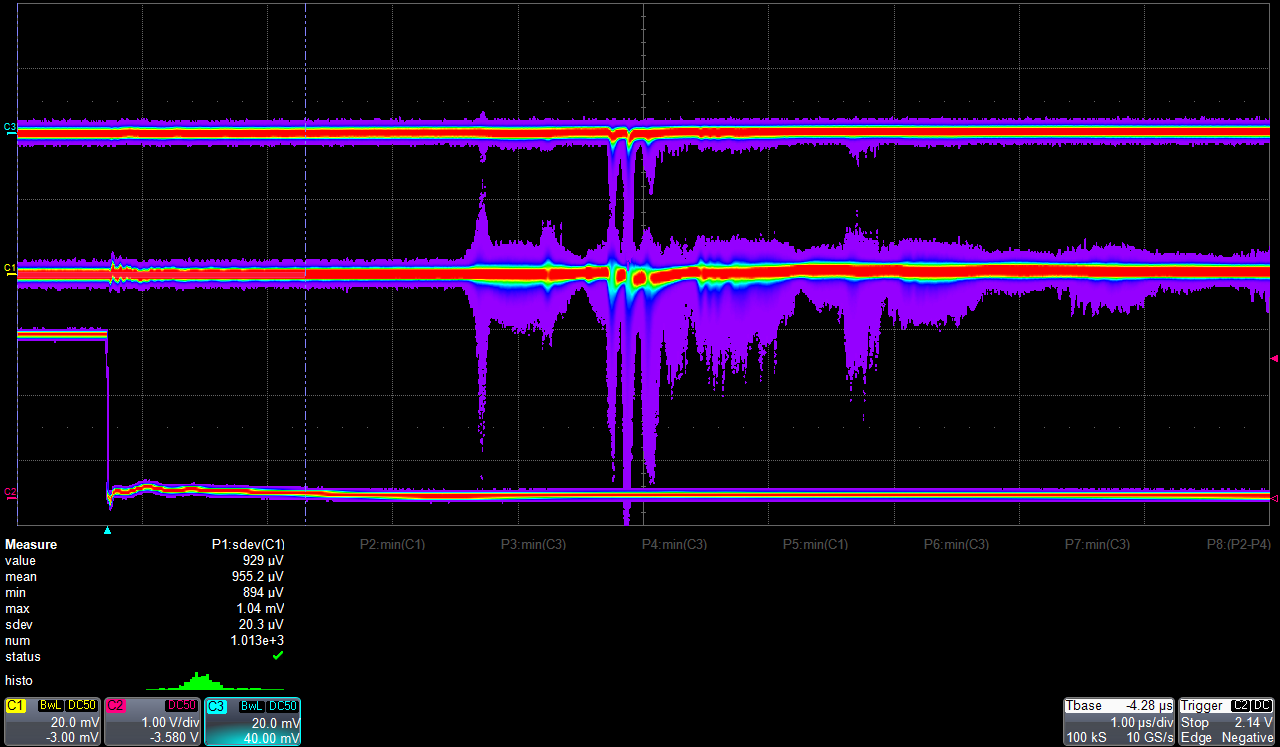
\includegraphics[totalheight=0.3\textwidth,trim=0.3cm 6.6cm 0.1cm 0cm, clip=true]{../Pictures/Pictures_oscilloscope/bad_noise.png}
  \caption{Electronic noise from radio frequency light leaks disturbs signals from the photo-detectors: pulse shapes will be 
  hided or deformed.Horizontal axis is 1$\Pmu$s/div and Vertical axis is 5mv/div.}
  \label{fig:noise_signal}
  \end{figure}
  
  \subsubsection{\textit{\underline{Sources of electromagnetic noise}}}
  
  We have noticed that electronic noise comes from electromagnetic sources:

  \begin{itemize}
  \item Some devices were not grounded. The signal from the photo-detectors oscillates \ref{fig:noise_signal}
  \item When the \xfl is working it is creating some radio waves which propagate through the air and are then transmitted to any piece of conductive metal of the 
  box. The consequences are : 
    \begin{itemize}
    \item The aluminum lid of the box conducts everywhere the electric field of these radio waves, which disturb the amplifiers.
    \item Each detector could feel these radio waves and the signal got worst.
    \item The metal divider acts as a transmitter and the piece of metal of the signal wires connected to the amplifiers acts as antenna.
    \end{itemize}
  \end{itemize}
  
  \subsubsection{\textit{\underline{Three main solutions}}}
  
  The first solution is to create a ground point on which all devices - especially the square wave pulse generator - are connected with the same wire 
  (to avoid ground loops). In that way, the oscillations of \ref{fig:noise_signal} are removed. 
  
  \paragraph{\underline{\emph{Isolate the lid from the box}}}
  
  As it is described above, the electric field from the radio waves propagates through the entire lid. When the box is closed 
  the electric field disturbs the operating 
  amplifiers. The solution is to isolate the lid from the box by adding black tape and, to guide the electric field, by adding copper on the edge of the lid
  to the ground point.

  \paragraph{\underline{\emph{Isolate the \xfl}}}
  
  As the \xfl creates radio waves, we decided to isolate it by building a Faraday cage around it. We added a thick piece of metal to absorb radio waves 
  and we covered this first part of the box with aluminum foil. In that way the electric field propagates through the aluminum foil to the edge of the top
  box to the ground point. 

  \paragraph{\underline{\emph{Isolate the photo-detectors and the amplifiers}}}
  
  The wire which connects a photo-detector to an amplifier seems to act like an antenna and transmits radio waves. A solution has been 
  to enroll such a wire with aluminum foil. The amplifier and the ground of the photo-detector are connected due to the aluminum foil.\\
  Another solution is to isolate the photo-detectors on the top and on the bottom by building Faraday cage around them.
    
  Those pictures below could summarize our work (yellow signal is the photo-detector on the bottom while the blue one is from the 
  photo-detector on the top):
  
  \newpage
  
  \begin{figure}[!hbtp]
  \centering
    \begin{subfigure}[A thin copper foil allows good contact between the lid and the top of the box.]{%
      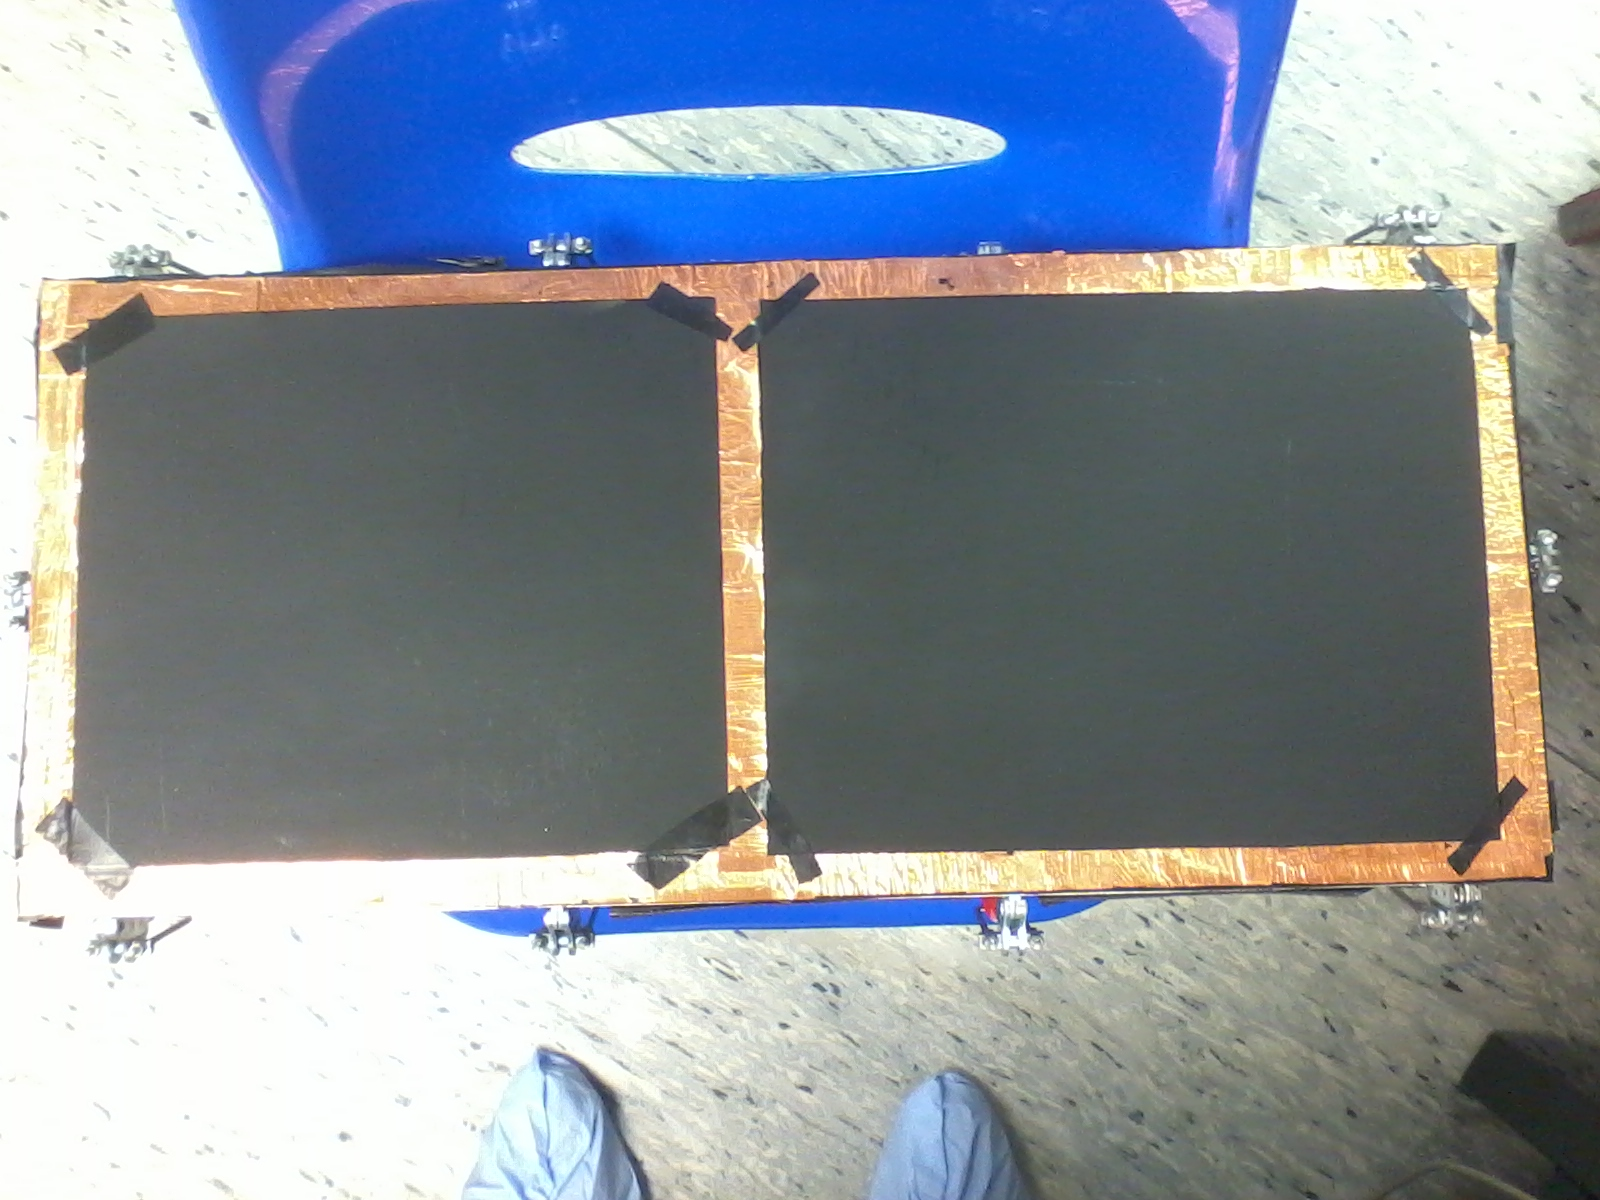
\includegraphics[totalheight=.27\textwidth,trim=0cm 10cm 1cm 8cm, clip=true]{../Pictures/Pictures_Setup/isolate_lid.jpg} 
      \label{fig:bad_noise}}
    \end{subfigure}
  \quad  
    \begin{subfigure}[A Faraday cage around each photo-detector isolates them from radio frequency leaks.]{%
      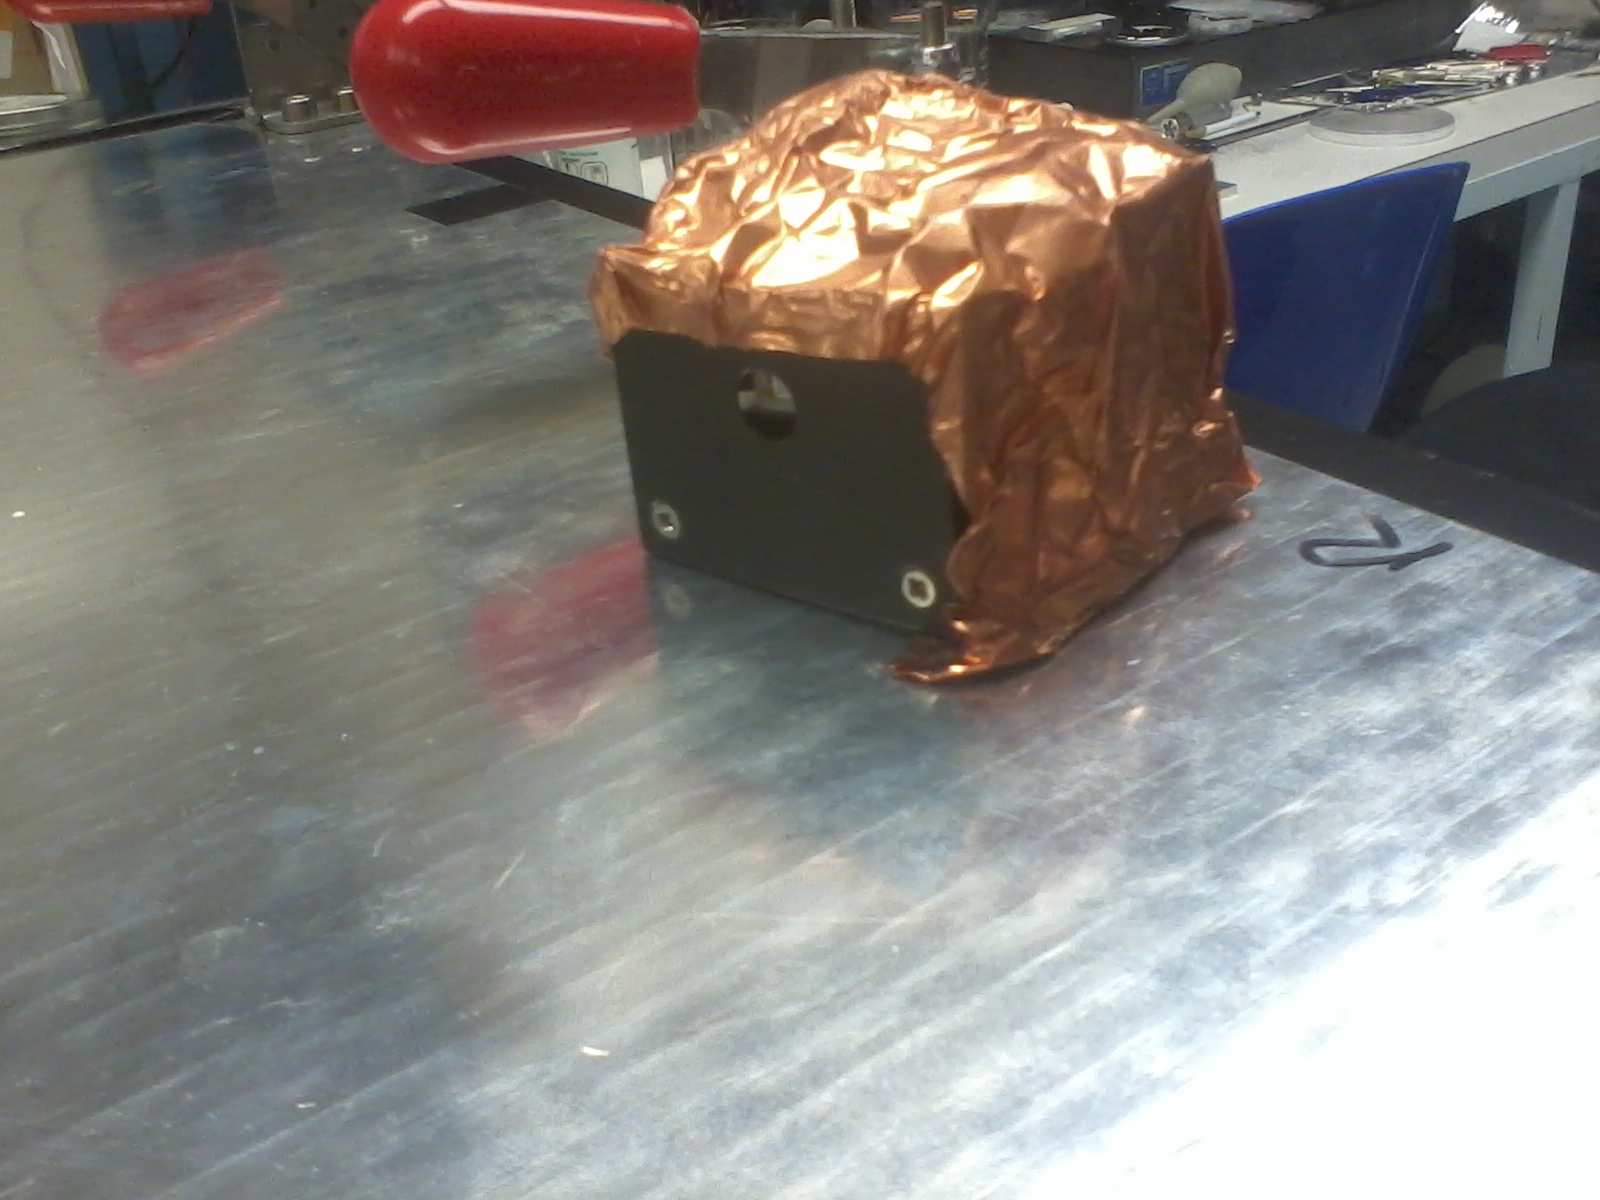
\includegraphics[totalheight=.27\textwidth,trim=20cm 18cm 11cm 2cm, clip=true]{../Pictures/Pictures_Setup/isolate_top.jpg}
      \label{fig:good_noise}}
    \end{subfigure}
  \quad  
  \begin{subfigure}[Each signal wire is enrolled with aluminum foil touching the ground part of each photo-detector.]{%
    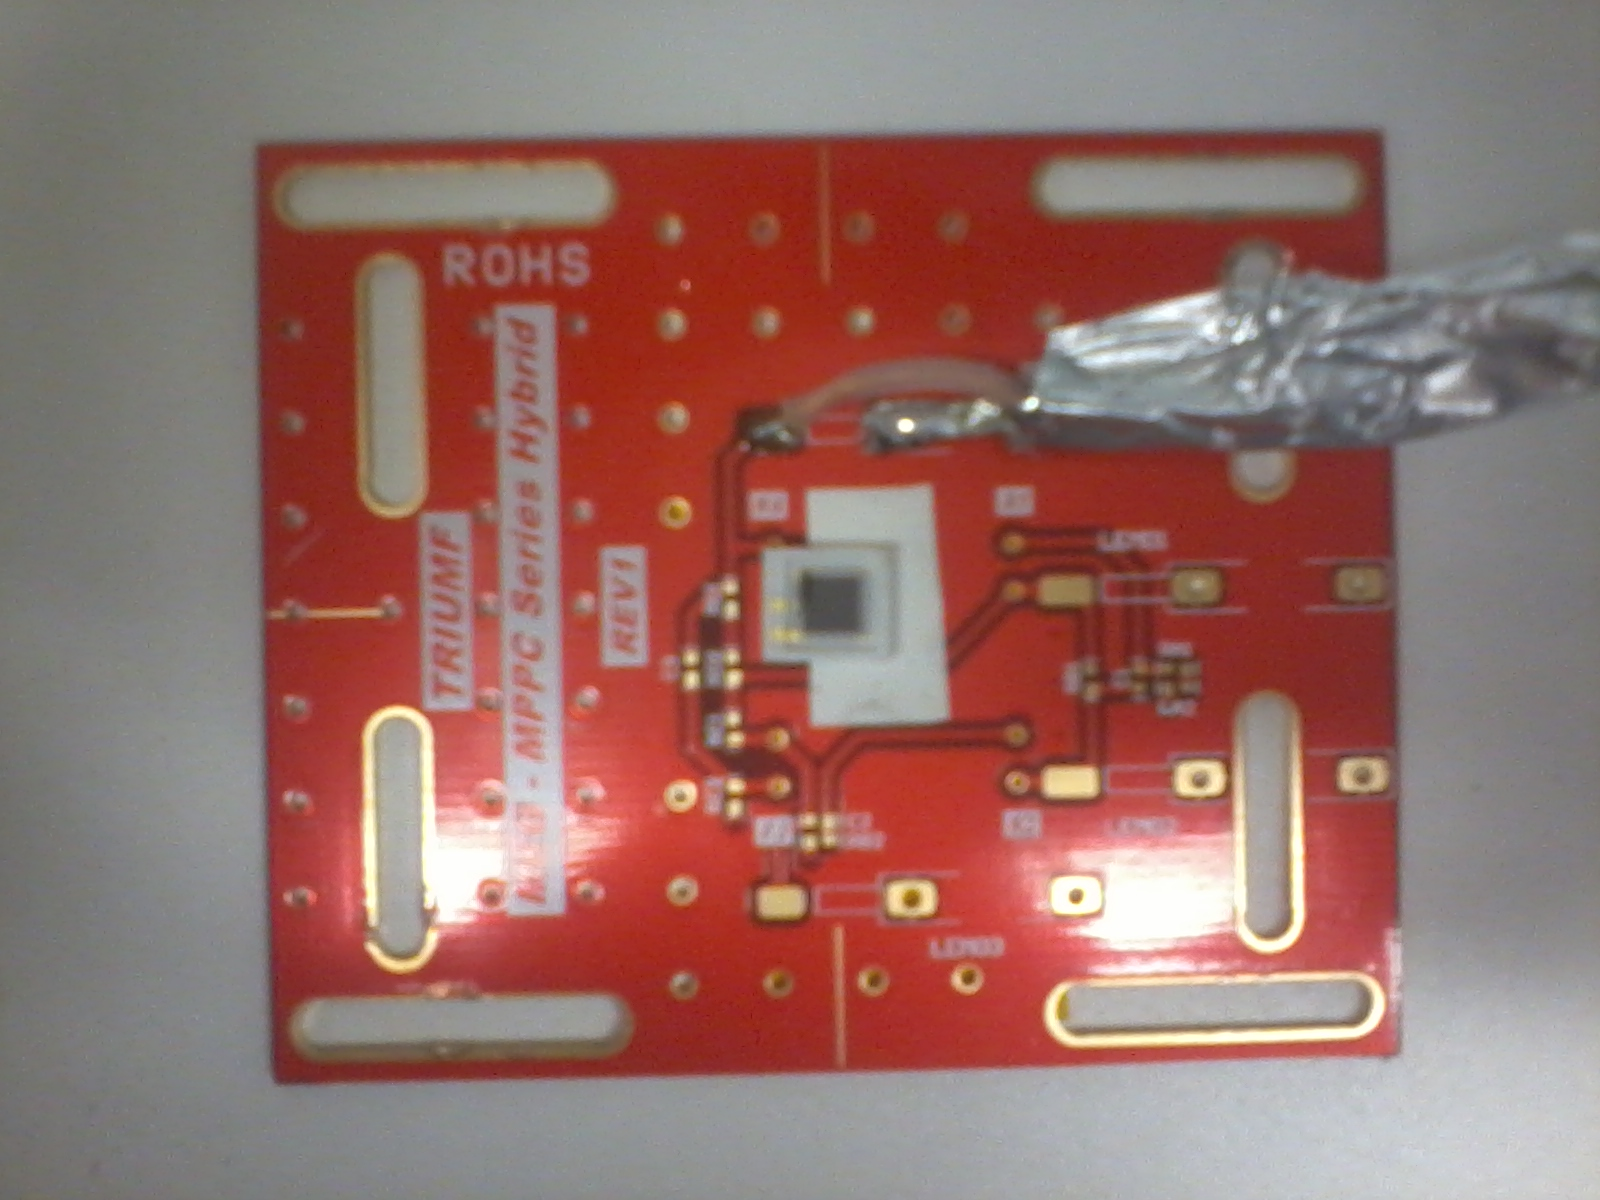
\includegraphics[totalheight=.27\textwidth,trim=8cm 3cm 4cm 4cm, clip=true]{../Pictures/Pictures_Setup/VUV3_2.jpg}
    \label{fig:good_noise}}
  \end{subfigure}
  \quad  
  \begin{subfigure}[Without electronic noise pulse shapes can be identified from Gaussian noise. 
  Horizontal axis is 1$\Pmu$s/div and Vertical axis is the amplitude (5mv/div).]{%
    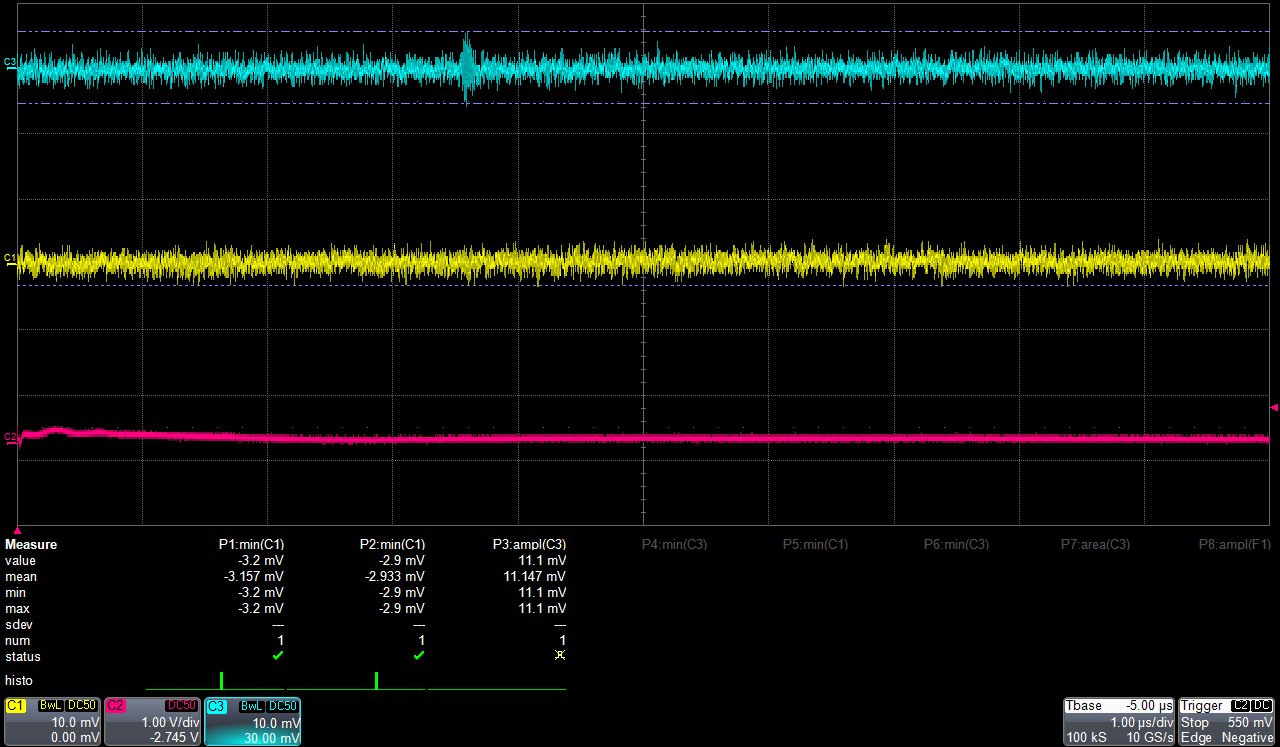
\includegraphics[totalheight=.2\textwidth,trim=0.3cm 6.6cm 0.1cm 0cm, clip=true]{../Pictures/Pictures_oscilloscope/good_elec_noise.jpg}
    \label{fig:good_noise}}
  \end{subfigure}
  \caption{Different technical solutions to clean signals of the photo-detectors from electronic noise.}
  \label{fig:noise_level}
  \end{figure}
    
  A SiPM, placed on the top, is used as a reference. It let us check if the light reminds constant when we characterize a MEG MPPC or a VUV3 SiPM at 
  $-100^\circ$C.
    
  \section{Efficiency of the photo-detectors}\label{sec:PE}
  
  Measuring the efficiency of the SiPM is one of the most important test to characterize them. 
  A paper from nEXO \cite{ref:charac_SiPM_nEXO} and another one \cite{ref:charac_SiPM} described how to measure the efficiency
  of SiPMs but not in our working experimental conditions: the wavelength of light is 175 nm and the efficiency has been calculated at 
  $-100^\circ$C. 
  
  \subsection{Methodology used to calculate efficiency}
  
  \subsubsection{\textit{\underline{Theoretical calculation}}}

  
  The previous paper from nEXO \cite{ref:charac_SiPM_nEXO} allows calculating the theoretical efficiency.\\
  A simple way to calculate the efficiency is to define two regions in the scope: the ``dark region'' is the time before the \xfl 
  triggers and the ``light region'' is the time immediately after the flash lamp triggers. So pulse shapes triggered by 
  photons can only appear on the light region.\\
  The both regions has the same size - 3$\Pmu$s \footnote{Time base is 1$\Pmu$s/div} each - to allow comparing those two regions. 
  The section \ref{subsubsec:DN_photon_shape} reminds that pulses triggered by photons or by hot carriers (dark noise) have the same shape. 
  Moreover pulse shapes from dark noise can appear anywhere in those two regions: 
  
  \begin{figure}[!hbtp]
    \centering
    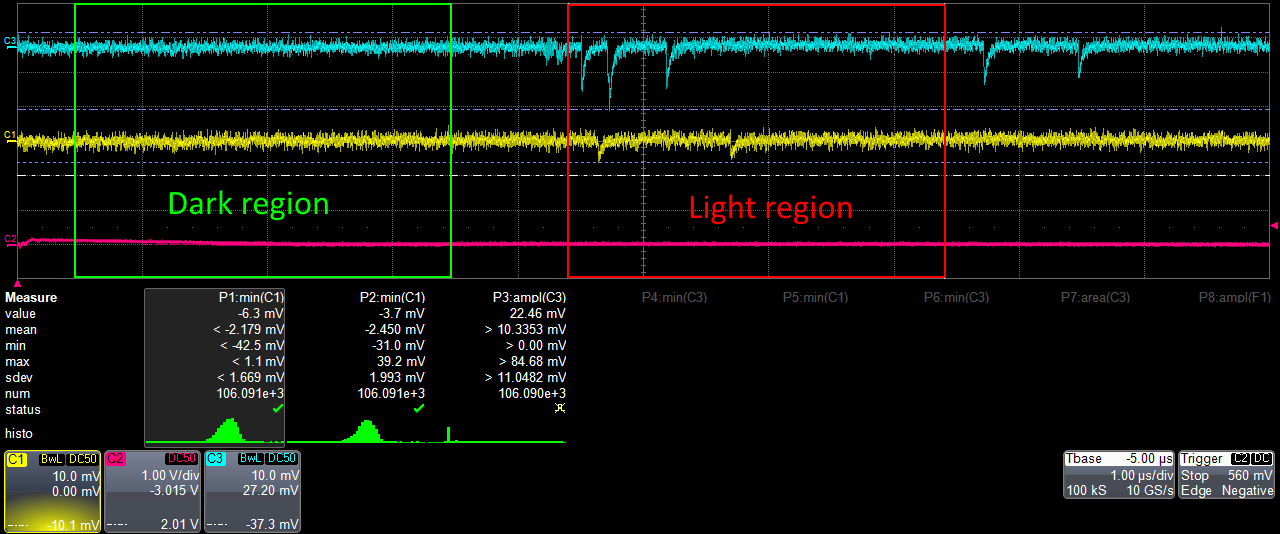
\includegraphics[totalheight=0.2\textwidth,trim=0.3cm 6.6cm 0.1cm 0cm, clip=true]{../Pictures/blabla/light_region_3.png}
    \caption{Dark and light regions.Horizontal axis is 1$\Pmu$s/div) and Vertical axis is 10mv/div.}
    \label{fig:dark_light_region}
  \end{figure}
  
  
  The average number of Photon Electron (which is the efficiency) - \(<PE>\) - of a photo-detector is defined with this relation below: 
  \\
  
  The probability of observing zero photon in the ``light region`` is : 
  
  \begin{equation}
    P_{L0} = \frac{N_{L0}}{N_{tot}} \textrm{,}   
  \end{equation}
  
  The probability of observing zero photon in the ''dark region`` is : 
  \begin{equation}
    P_{D0} = \frac{N_{D0}}{N_{tot}} \textrm{,}
  \end{equation}
  
  where \(N_{L0}\) is the number of times of not observing any pulses in the ''light region`` and \(N_{D0}\) is the number of time of not observing 
  any pules in the ''dark region``. 
  \(N_{tot}\) is the total number of events. 
  
  The probability of obtaining zero dark noise \(P_{DN0}\) and the probability of obtaining zero photo electron from the lamp \(P_{Lamp0}\)
  follow a Poisson distribution. These two probabilities are linked by the probability \(P_{L0}\): 
  
  \begin{equation}\label{eq:Poisson_law}
    P_{L0} = P_{Lamp0}.P_{DN0} \textrm{, where } P_{Lamp0} = \mathrm{e}^{-<PE>} \textrm{ and } P_{DN0} = \mathrm{e}^{-DN}
  \end{equation}
  \begin{equation}
    \textrm{So : } \mathrm{e}^{-<PE>} =\frac{P_{L0}}{P_{D0}}
  \end{equation}
  
  \begin{equation}
    <PE> =  -ln(\frac{P_{L0}}{P_{D0}}).
  \end{equation}
  
  \subsubsection{\textit{\underline{Setting and analysis}}}
  
  On the scope we trigger on the lamp. The scope displays a waveform on 10$\Pmu$s since the \xfl is on during 10 $\Pmu$s (with a frequency of 100Hz)\\
  During this lapse of time,we noticed that the lamp needs more than 4$\Pmu$s before sending photons. After 4$\Pmu$s we could noticed 
  pulse shapes triggered by photons.\\
  Also as it is shown on these screen-shots of the oscilloscope \ref{app:tests} the voltage set on the lamp influence the position 
  in time of pulse shapes triggered by photons. Moreover the pulse shape of the lamp \ref{app:setup} lasts around 1.4$\Pmu$s which means that 
  most of such pulse shapes will appear in that lapse of time \ref{app:tests}. So the size of the ''light and dark region`` could have
  been set at around 1.4$\Pmu$s. 
  For example, with a window size of 3$\Pmu$s, the dark region begins at 0.9$\Pmu$s and end at 3.9$\Pmu$s while the light region 
  begins at 5$\Pmu$s and end at 8$\Pmu$s.
  \\
  
  The oscilloscope is monitored and it is possible to record, on the same time, a predefined number of waveform 
  (we choose 15000 waveforms). 
  \\
  
  The C++ code ''efficiency.exe`` smooths a waveform (to decrease the Gaussian noise and increase the ratio Signal/Noise),
  records the minimum of it in each regions and plots an histogram which allows counting the number of 
  zero photon electron (0PE) in the ''light and dark region``.
  \\
  
  Here is an example of line command: \textit{bin/efficiency.exe -r 1733 -s 10 -w 3000 -b 900 -a 5000},\\
  with ''-r`` is for the number 
  of the \textit{run}, ''-s`` to set the \textit{smoothing}, ''-b`` to set the beginning of the ''dark region``, \textit{before} 
  pulses triggered by photons and ''-a`` to set the beginning of the ''light region``, \textit{after} pulses triggered by photons.
  
  
  
  \subsection{Inconsistent results at $-100^\circ$C}
  
  Here is one of our results for the VUV3 SiPM at $-100^\circ$C with an over-voltage of 5V (At such temperature the breakdown voltage 
  is 44.73V). The appendix \ref{app:tests} could explain how to calculate the breakdown voltage for each device at different temperatures. 
  \\
  
  The histogram below shows from right to left zero photon electron (0PE), one photon electron (1PE):   
  
  \newpage

  \begin{figure}[!hbtp]
    \centering
    \includegraphics[totalheight=0.4\textwidth,trim=2.8cm 5.15cm 3.5cm 4cm, clip=true, page = 34]{../nEXO_Photomultiplier_Test_Setup.pdf} 
    \caption{Histogram of VUV3 SiPM for an over-voltage of 5V @ $-100^\circ$C.}
    \label{fig:histo_PE}
  \end{figure}

  
  Severals tests on the same experimental conditions are made to see if our results for the VUV3 SiPM are reproducible:
  
  \begin{figure}[!hbtp]
  \centering
  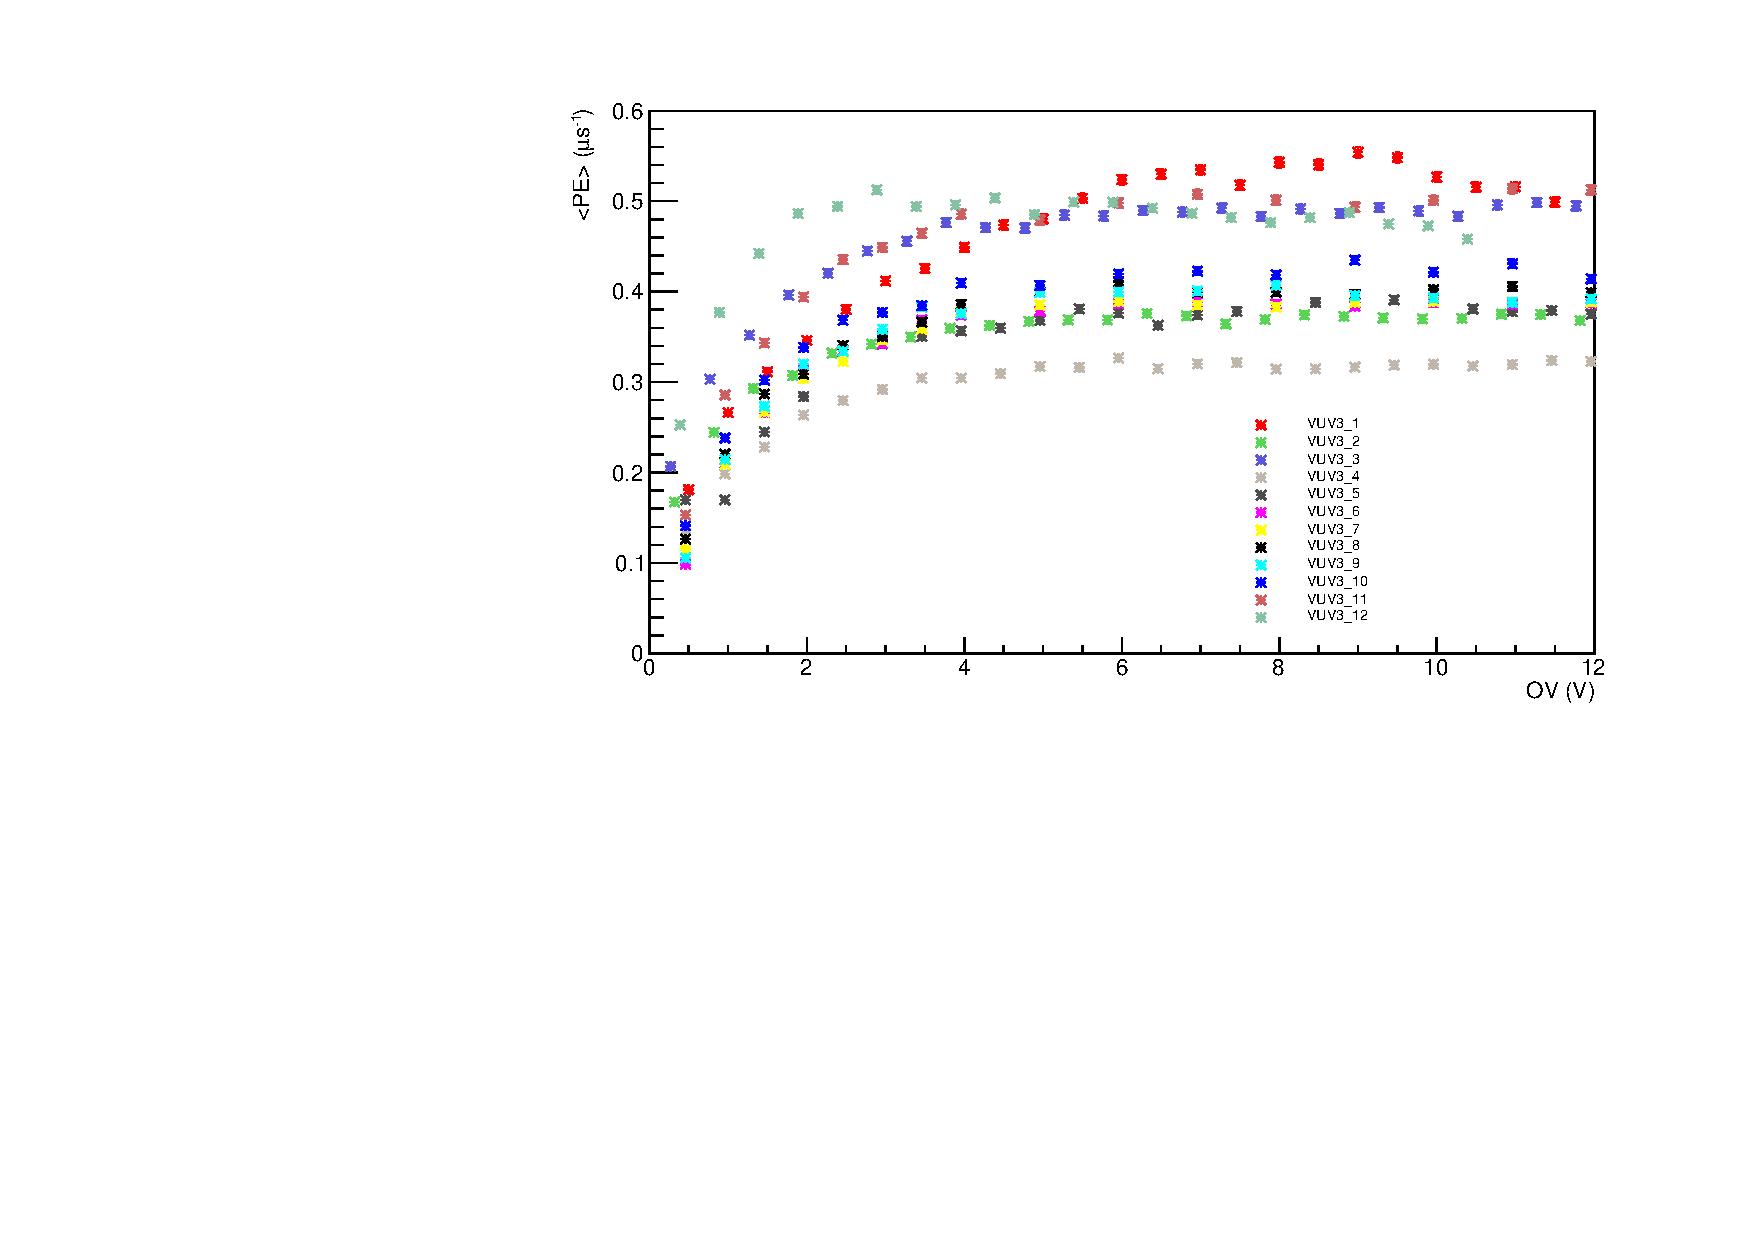
\includegraphics[totalheight=0.5\textwidth,trim=0.5cm 0cm 1.8cm 0.5cm, clip=true]{../Pictures/VUV3_paul.pdf}
  \caption{Inconsistent results for the efficiency of the VUV3 SiPM at $-100^\circ$C.}
  \label{fig:issue}
  \end{figure}
  
  The error bars are quiet small (the appendix \ref{app:tests} details the error bars calculation.) 
  
  \subsection{Analysis: the misalignment of the light}
  
  We would like to count the number of time we see a pulse corresponding to 1PE peak. 1PE peak can come from a single pixel 
  avalanches triggered by photons or from avalanches triggered by hot carriers (dark noise).\\
  Moreover in the light region it is not possible to make the difference between a pulse shape triggered by a photon or by hot carriers. 
  One solution is to take in account pulse shapes from dark noise in the ''dark region``.
  In that region we know for sure that 1PE peak comes obviously from dark noise.\\
  Considering the fact that dark noise in the light region or in the dark region appears at the same rate \ref{eq:Poisson_law},
  a solution will be to divided the 0PE peak of the ''light region`` by the 0PE peak from the dark region.\\
  The function -ln- comes from the Poisson distribution.
  \\
  
  Whatever is the run the efficiency increases as ln function. Moreover when we increase the reversed voltage of a photo-detector, 
  the probability of observing crosstalk increases (so the 2 PE peak increases) and thus the probability of observing 
  0PE peak decreases for a same number of waveforms. So the number 0PE peak from the ''light region`` decreases faster than the one 
  from the ''dark region``, which explains those ln variations. 
  \\
  
  Nevertheless such observations don't explain such an inconsistency of the efficiency at $-100^{\circ}$C.\\
  We made those different runs with the same VUV3 SiPM. So at the same temperature, the breakdown voltage is the same. 
  Five parameters could explain such an inconsistency:
  
  \begin{itemize}
   \item The voltage of the lamp, 
   \item The quantity of oxygen inside the box, 
   \item Dust on the area of the photo-detectors,
   \item The size of the screen of the oscilloscope,
   \item The alignment of the photo-detectors with the beam of light.
  \end{itemize}

  \subsubsection{\textit{\underline{The fourth first parameters}}}

  The voltage of the lamp has two impacts on the efficiency.\\
  First when the voltage is increasing the \xfl sends more light and so 
  more photons trigger avalanches inside an SiPM. According to the previous section, the efficiency decreases.
  Second as explained previously the voltage of the lamp influence the position in time of pulse shapes triggered by photons.\\  
  So if the voltage of the lamp changes between each run, the ''light and dark region`` will change also and so the efficiency will change for 
  a same over voltage of a photo-detector.\\  
  Nevertheless we set the voltage of the lamp at 2.8V for each run. The setting for the ''light and drak region`` is described above.  
  \\
  
  The quantity of oxygen inside the box could have an impact on the efficiency. The box is filled with N2 to allow propagation of photons
  from the lamp to the detectors. It also lets avoid frost on the area of the photo-detectors cooled on the bottom of the box. 
  So far no frost has been observed but the quantity of oxygen inside the box has not been checked. 
  \\
  
  On the contrary we have already seen some dust on the area the photo-detectors. Run 2 and run 3 \ref{fig:issue} show that reality. During the 
  run 2 some dust was on the area of the photo-detector on the bottom while dust was blowed out for the next run (run 3). 
  \\
  
  The windows size of the screen of the oscilloscope has an influence on the efficiency. Indeed the increasing voltage applied on 
  the photo-detectors increases the height of any pulse shapes. At low voltage all pulse shapes (especially crosstalk since pulses 
  from crosstalk are at least twice higher than 
  pulse shape from single pixel avalanches) are not cut by the windows size (5mV/div). At high voltage all pulse shapes are cut 
  by such a small window size and thus histograms will not let make the difference between 0PE, 1PE, 2PE ...\\
  That is why the windows size needs to be adjust when the voltage of the photo-detectors changes.
  
  \subsubsection{\textit{\underline{Effect of the temperature}}}

  
  To check if the efficiency of the two photo-detectors reminds constant over the time at $-100^\circ$C, four run are made. 
  We have also 
  noticed that the beam splitter seems to move at such low temperature (which means that temperature seems to have an impact on the 
  beam splitter). For that here are the parameters we changed between different runs:
  
  \begin{itemize}
   \item run 1: @ $-100^\circ$C, with beam splitter,
   \item run 2: @ $-100^\circ$C, without beam splitter,
   \item run 3: @ RT, with beam splitter,
   \item run 4: @ RT, without beam splitter.
  \end{itemize}

  The other parameters remind the same between different runs : the over-voltage and the position of the photo-detectors \footnote{For 
  the bottom one, the over-voltage is different at RT than at  $-100^\circ$C since the breakdown voltage decreases with temperature \ref{app:tests}}, the voltage and the position of the lamp, the box filled with N2 and the stabilization
  of the temperature at $-100^\circ$C (wait at least 30 min for that).\\
 
  \begin{figure}[!hbtp]
    \centering
    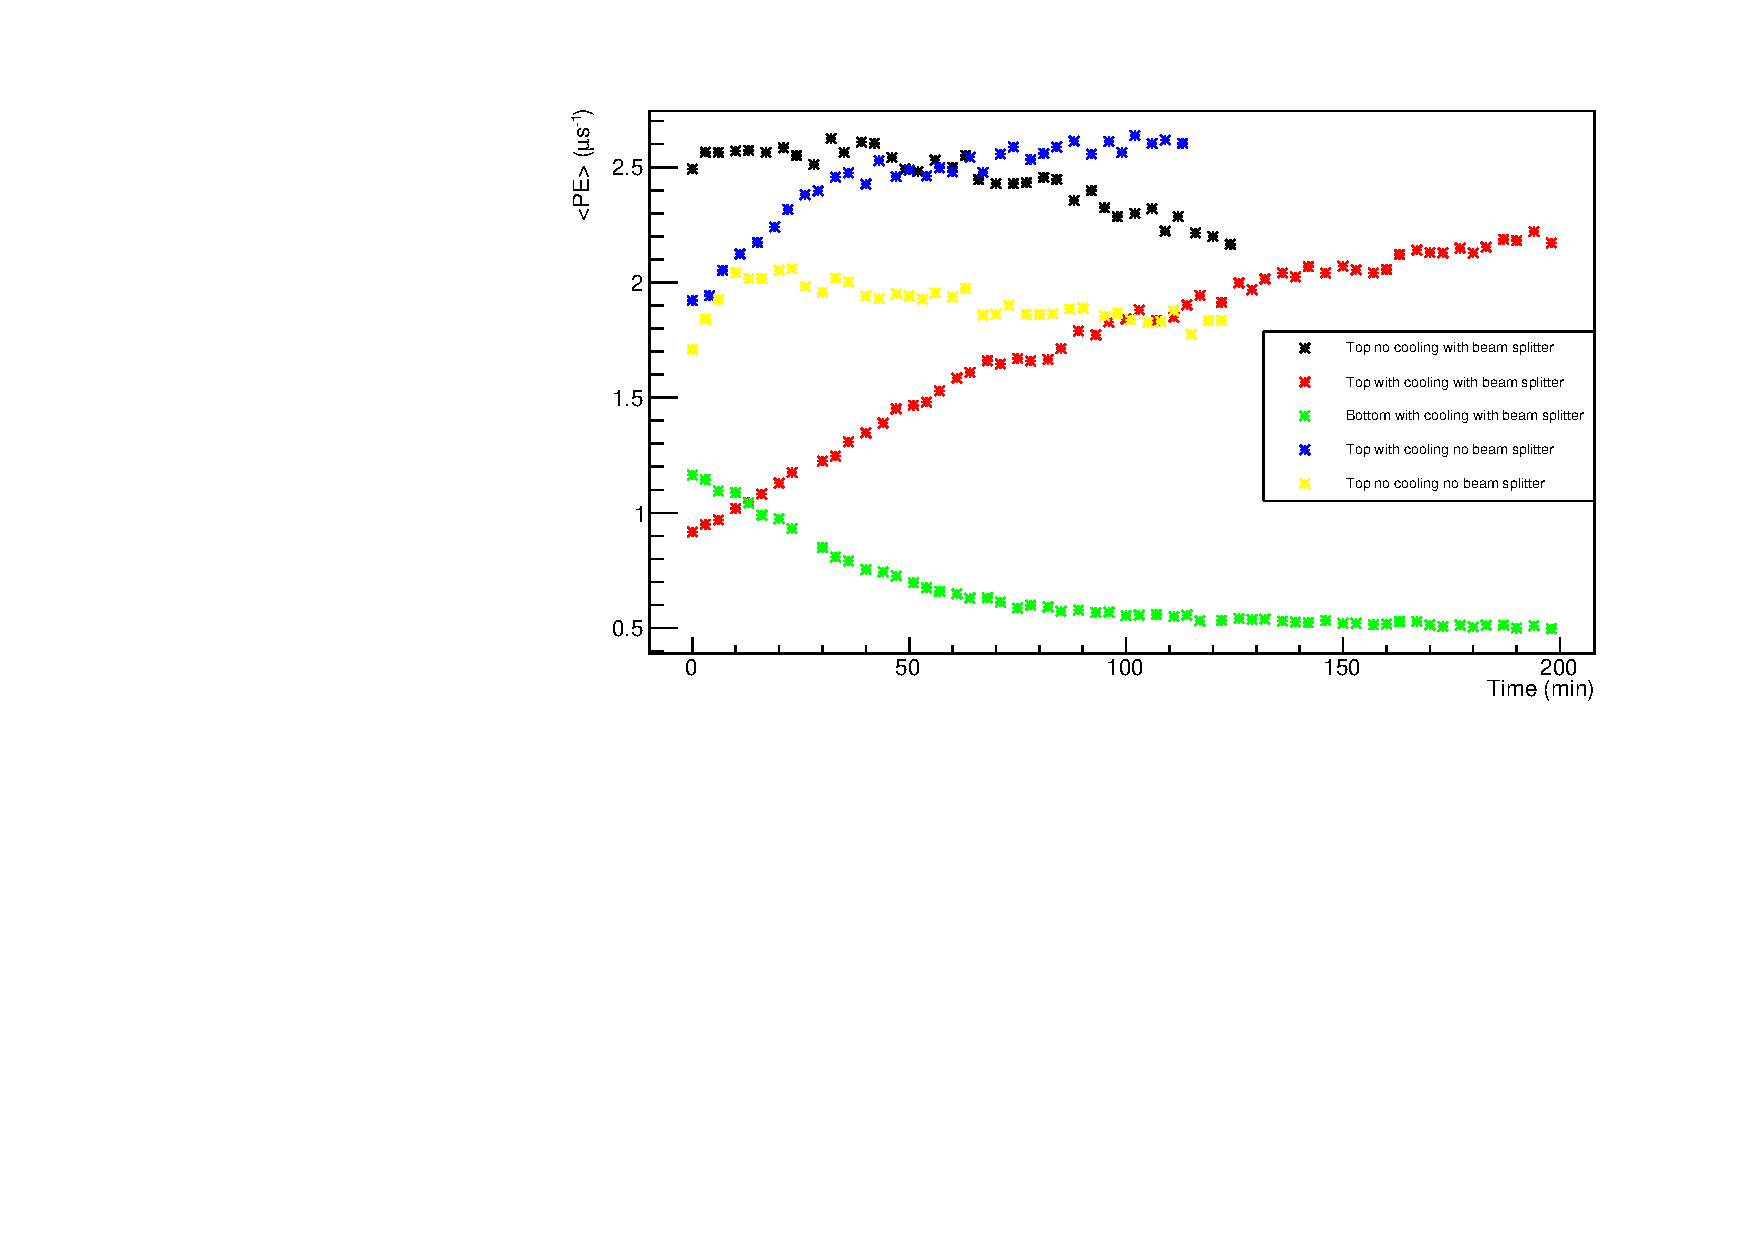
\includegraphics[totalheight=0.55\textwidth,trim=0.5cm 0cm 1.8cm 0.5cm, clip=true]{../Pictures/NewLampPEAug5.pdf}
    \caption{Hugh variations of the efficiency for the top and bottom after three hours of running.}
    \label{fig:hugh_variation}
  \end{figure}
  
  \newpage
  
  So far the alignment of the beam splitter with both of the photo-detectors seems to be the main reason to explain the previous plot. 
  The picture below shows what is going on while cooling @ $-100^\circ$C:
  
  \begin{figure}[!hbtp]
  \centering 
  \begin{tikzpicture}[scale = 1]%, show background rectangle]
    \draw(0,0) rectangle (11,5);%(x,y)
    %oder has importance 
    
    \draw[|, black!80, line width=1pt] (6.55,1.2)--(6.55,2.5);
    \draw[-, black!80, line width=1pt] (6.54,2.5)--(7.25,2.5);
    \draw[|, black!80, line width=1pt] (7,2.8)--(7,2.5);
    \draw[|, black!80, line width=1pt] (7.25,2.88)--(7.25,0.88);
    \draw[-, black!80, line width=1pt] (0,0.88)--(11,0.88) node at (6,0.4) {\color{black} \textbf{$Bottom\ of\ the\ box$}};
    
    \draw[-,green,thick,dashed] (0,3.35) node[above right]{\color{black} $Beam \ @ -100^{\circ}$} -- (7.2,3.35) ;%cooling    
    \draw[-,red,thick,dashed] (0,3) node[below right]{\color{black} $Beam \ @ \ RT$} -- (7.2,3);%RT
    \draw[|,blue,line width=1.5pt] (7,4) -- (7,3.7);%collimator top top
    \draw[|,blue,line width=1.5pt] (7,2.8) -- (7,3.1);%collimator top bottom     
    \draw[black](7.2,2.9) rectangle (7.3,3.8); % top detector
    \draw (9,1.8) node at (9,2) {$Photodetectors$};
    \draw[->] (8,2.3) -- (7.4,3.35);%arrows to top
    \draw[->] (8,1.7) -- (6.6,1);% arrow to bottom
    
    \draw[-,green,thick,dashed] (5.66,3.35) -- (5.66,1);%cooling    
    \draw[-,red,thick,dashed] (6,3) -- (6,1);%RT
    \draw[-,blue,line width=1.5pt] (5.46,1.2) -- (5.76,1.2);%collimator top right
    \draw[-,blue,line width=1.5pt] (6.25,1.2) node at(4,1.2) {\color{blue} $Collimator$} -- (6.55,1.2);%collimator top left
    \draw[black](5.56,0.9) rectangle (6.45,1);% bottom detector 
    
    \draw[|, black!80, line width=1pt] (6.55,1.2)--(6.55,2.5);
    \draw[-, black!80, line width=1pt] (6.54,2.5)--(7.25,2.5);
    \draw[|, black!80, line width=1pt] (7,2.8)--(7,2.5);
    \draw[|, black!80, line width=1pt] (7.25,2.88)--(7.25,0.88);
    \draw[-, black!80, line width=1pt] (0,0.88)--(11,0.88) node at (6,0.4) {\color{black} \textbf{$Bottom\ of\ the\ box$}};
    
    
    \draw[-,black, thick] (5.2,3.8) -- +(315:1.9) node at(4.8,4.3) {$Beam splitter$};%bs
    
  \end{tikzpicture}    
  \caption{Effect of the temperature on the position of the two collimators.}
  \label{fig:effect_temp}
  \end{figure}

  The diameter of the hole of 1mm of each collimator is checked to be centered on the surface of each photo-detectors.
  \\
  
  First a board holds both of the collimators, the beam splitter and the photo-detector on the top, as shown on figure \ref{fig:effect_temp}. 
  The photo-detector on the bottom can move independently of the previous board.\\
  When the cooling system is working the temperature of the board decreases from $22^\circ$C to around $10^\circ$C 
  \footnote{Temperature of the box decreases from RT to around $15^\circ$C} after 2 hours of running.   
  \\
    
  The opposite alignment of the beam with the photo-detector on the top and on the bottom explains the anti-correlation observed on figure 
  \ref{fig:hugh_variation} (top/bottom with cooling and with beam splitter).\\
  Indeed we notice on \ref{fig:hugh_variation} that the efficiency for the  photo-detector on the top is lower on the beginning of the run 
  (The board is at room temperature) than at the end (The temperature of the board is around $10^\circ$C).The efficiency for the photo-detector
  on the bottom acts in opposite way.\\
  At room temperature (RT) the collimator (and so the photo-detector on the top since both are always centered) is not aligned with the beam
  of the \xfl. On the contrary the collimator on the bottom is aligned with the beam. When the board is cooling down over the time, 
  it moves a little bit. The consequence is that, at low temperature, the collimator on the top is aligned with the beam while the one on the bottom is no more
  aligned. This explains our previous results. 
  \\
 
  It is not only the beam splitter which moves over the time but all the board and so the collimator of the top and of the bottom.
  We could see
  that with run 2 (without beam splitter): we observe the same variation of efficiency for the photo-detector on the top (the efficiency 
  of the photo-detector on the bottom is quiet null since no light can reach its area without beam splitter). 
 
  \subsubsection{\textit{\underline{Conclusion}}}
  
  The misalignment of the light explains our inconsistent results. A solution should be to focus the beam of the \xfl on the collimator
  with a lens.   
  
  \section{Dark Noise rate}\label{sec:DN}
  
     
  \subsection{Methodology for dark noise}
  
  One of the main source of noise limiting the SiPM performance is the dark noise rate, which mainly originates from electrons 
  created thermally in the depletion region \ref{fig:PN_junction}. These carriers trigger avalanches exactly as 
  if pixels would have been fired by photons.
  
  \subsubsection{\textit{\underline{theoretical dark noise}}}

  
  To calculate the dark noise rate, the goal is to count the number of time the screen of the scope
  displays 1PE peak. A simple idea is 
  to record the minimum of pulses in ''the dark region`` \footnote{See section \ref{sec:PE}}.\\
  In the ''light region`` avalanches can be triggered by a photons or by hot carriers (dark noise) while in the dark region
  avalanches can be triggered only by hot carriers. But the probability of observing dark noise in the both regions is the same. 
  \\
  
  Here is the equation used to calculate the average number of dark noise $<DN>$:
  
  \begin{equation}
    <DN> = \ln{\frac{N_{D0}+N_{L0}}{2\cdot15000}},
  \end{equation}

  where $N_{D0}$ and $N_{L0}$ are the number of 0PE in the ''dark and light region`` , respectively. 15000 waveforms are recorded
  for each region of 1000$\Pmu$s. The total number of waveforms is $2\cdot15000 = 30000$ waveforms. 
  \\
  
  As described previously the dark noise rate follows a Poisson distribution:
  
  \begin{equation}\label{eq:DN_Poisson}
   P_{DN0} = \mathrm{e}^{-<DN>},
  \end{equation}

  where $<DN>$ and $P_{DN0}$ are the dark noise rate \footnote{The dark noise rate, in Hz, is the number of dark noise par second divided.} 
  of and the probability of not observing any pulses in the dark region, respectively. 
  \\
  
  \newpage
  
  \subsubsection{\textit{\underline{setting and algorithm}}}
 
  On the scope we trigger one the lamp and we record waveforms as described previously.\\  
    
  The C++ code ''fillNtp.exe`` smooths a waveform (to decrease the Gaussian noise and increase the ratio Signal/Noise),
  set two windows of 1$\Pmu$s each in the ''light and dark region'' and records the minimum of a waveform and plot an histogram. 
  
  Here is an example of line command: \textit{bin/fillNtp.exe -r 956 -s 10 -w 1000 -b 1500 -a 8500},\\
  with ''-r, -s, -b, -a`` are described above.   
  
  \subsection{Results}
  
  The histogram looks the same than the one of the previous section \ref{sec:PE}.
  \\
  
  The first goal is to plot the dark noise rate versus temperature. Moreover the over-voltage for each temperature must be the same 
  since the over-voltage applied on the photo-detector changes pulse shapes. The appendix \ref{app:tests}
  explains how we proceed to calculate the breakdown voltage for the VUV3 SiPM.\\
  We worked with low over-voltage to avoid crosstalk and the previous histograms allow plotting the dark noise rate $<DN>$ versus 
  temperature since the dark noise depends of the temperature 
  \ref{subsubsec:DN_photon_shape}:
  
  \begin{figure}[!hbtp]
  \centering
    \begin{subfigure}[The fitting allows finding a breakdown voltage of 44.73V for the VUV3 SiPM at $-100^{\circ}$C.]{%
      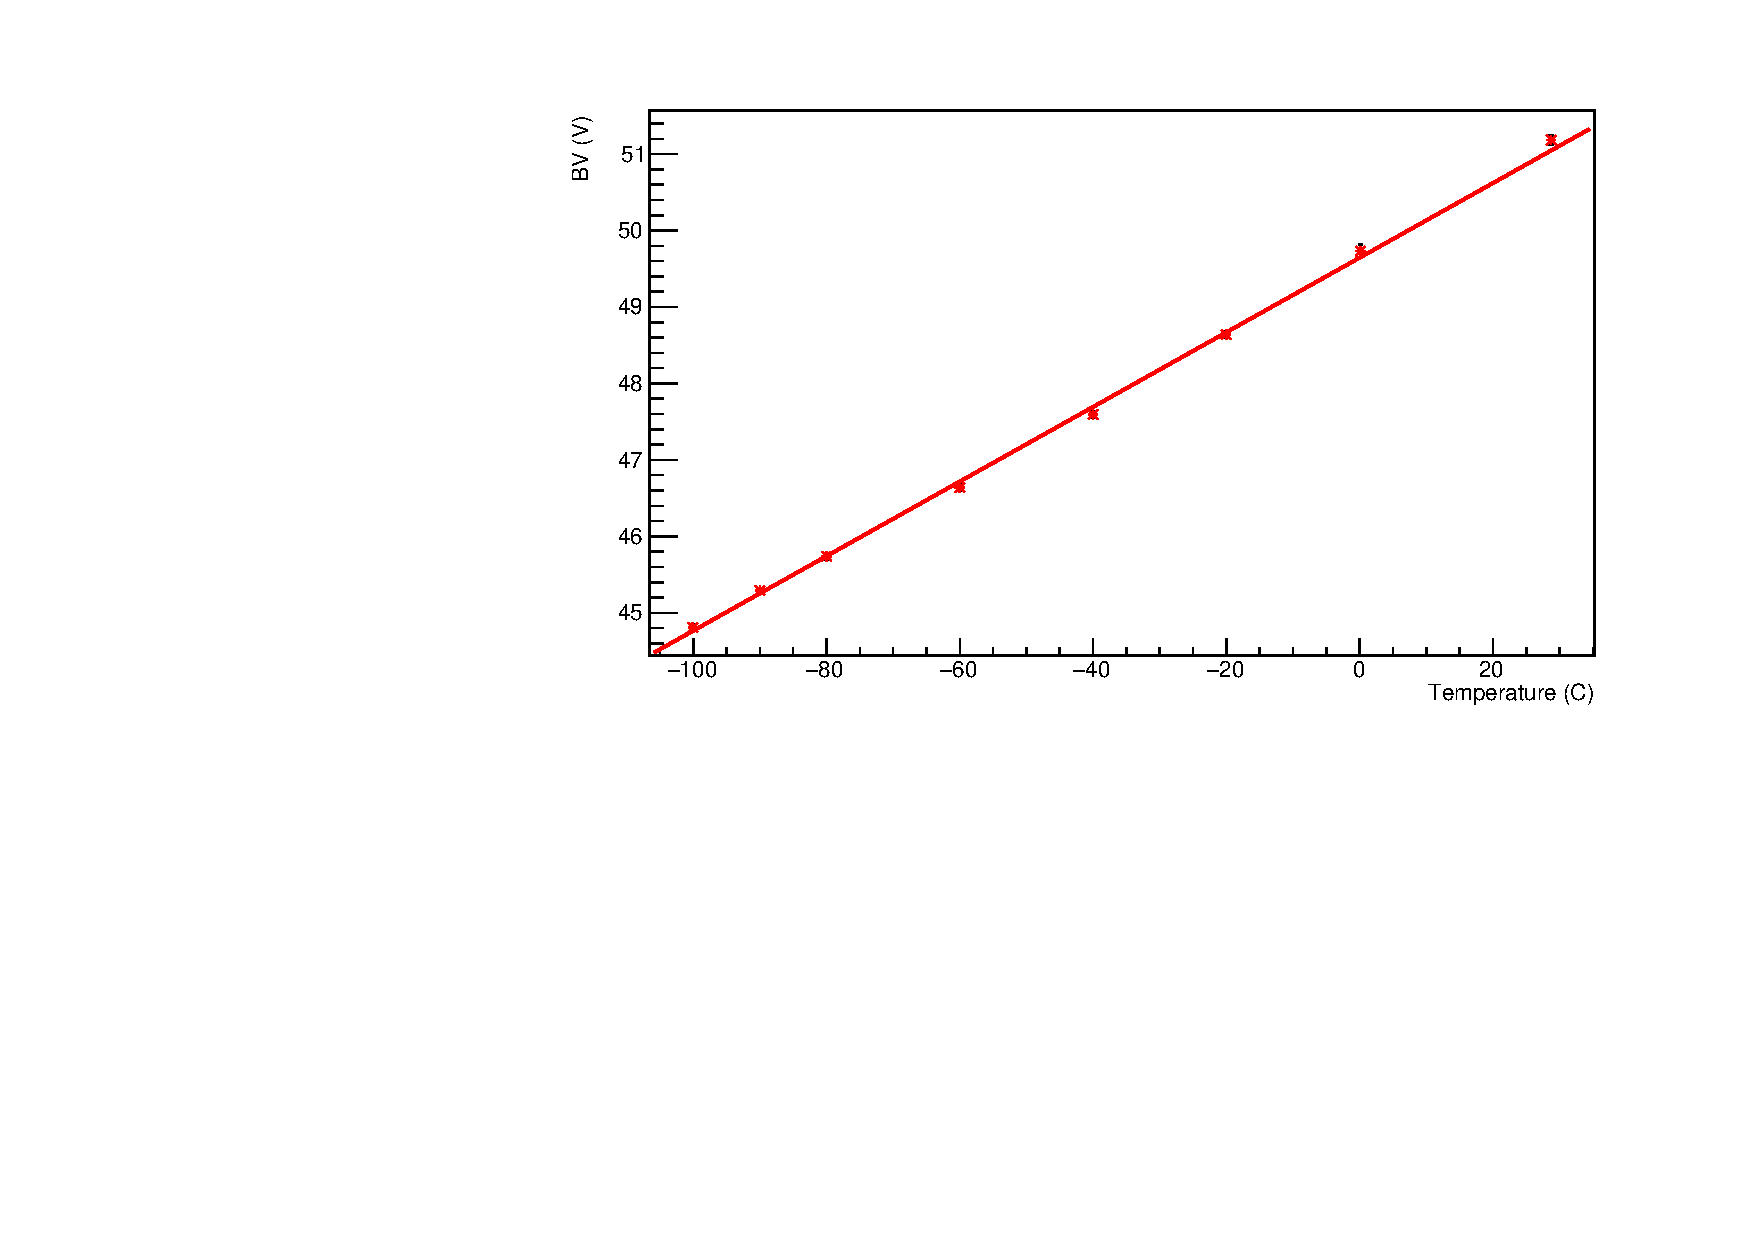
\includegraphics[totalheight=0.27\textwidth,trim=0.5cm 0.2cm 1.5cm 1cm, clip=true]{../Pictures/BV_temp.pdf}
      \label{fig:BV_VUV3_SiPM_vs_temp}}
    \end{subfigure}
  \quad  
    \begin{subfigure}[Dark noise rate versus temperature for the \textcolor{blue}{VUV3 SiPM} and the \textcolor{red}{MEG MPPC}.]{%
      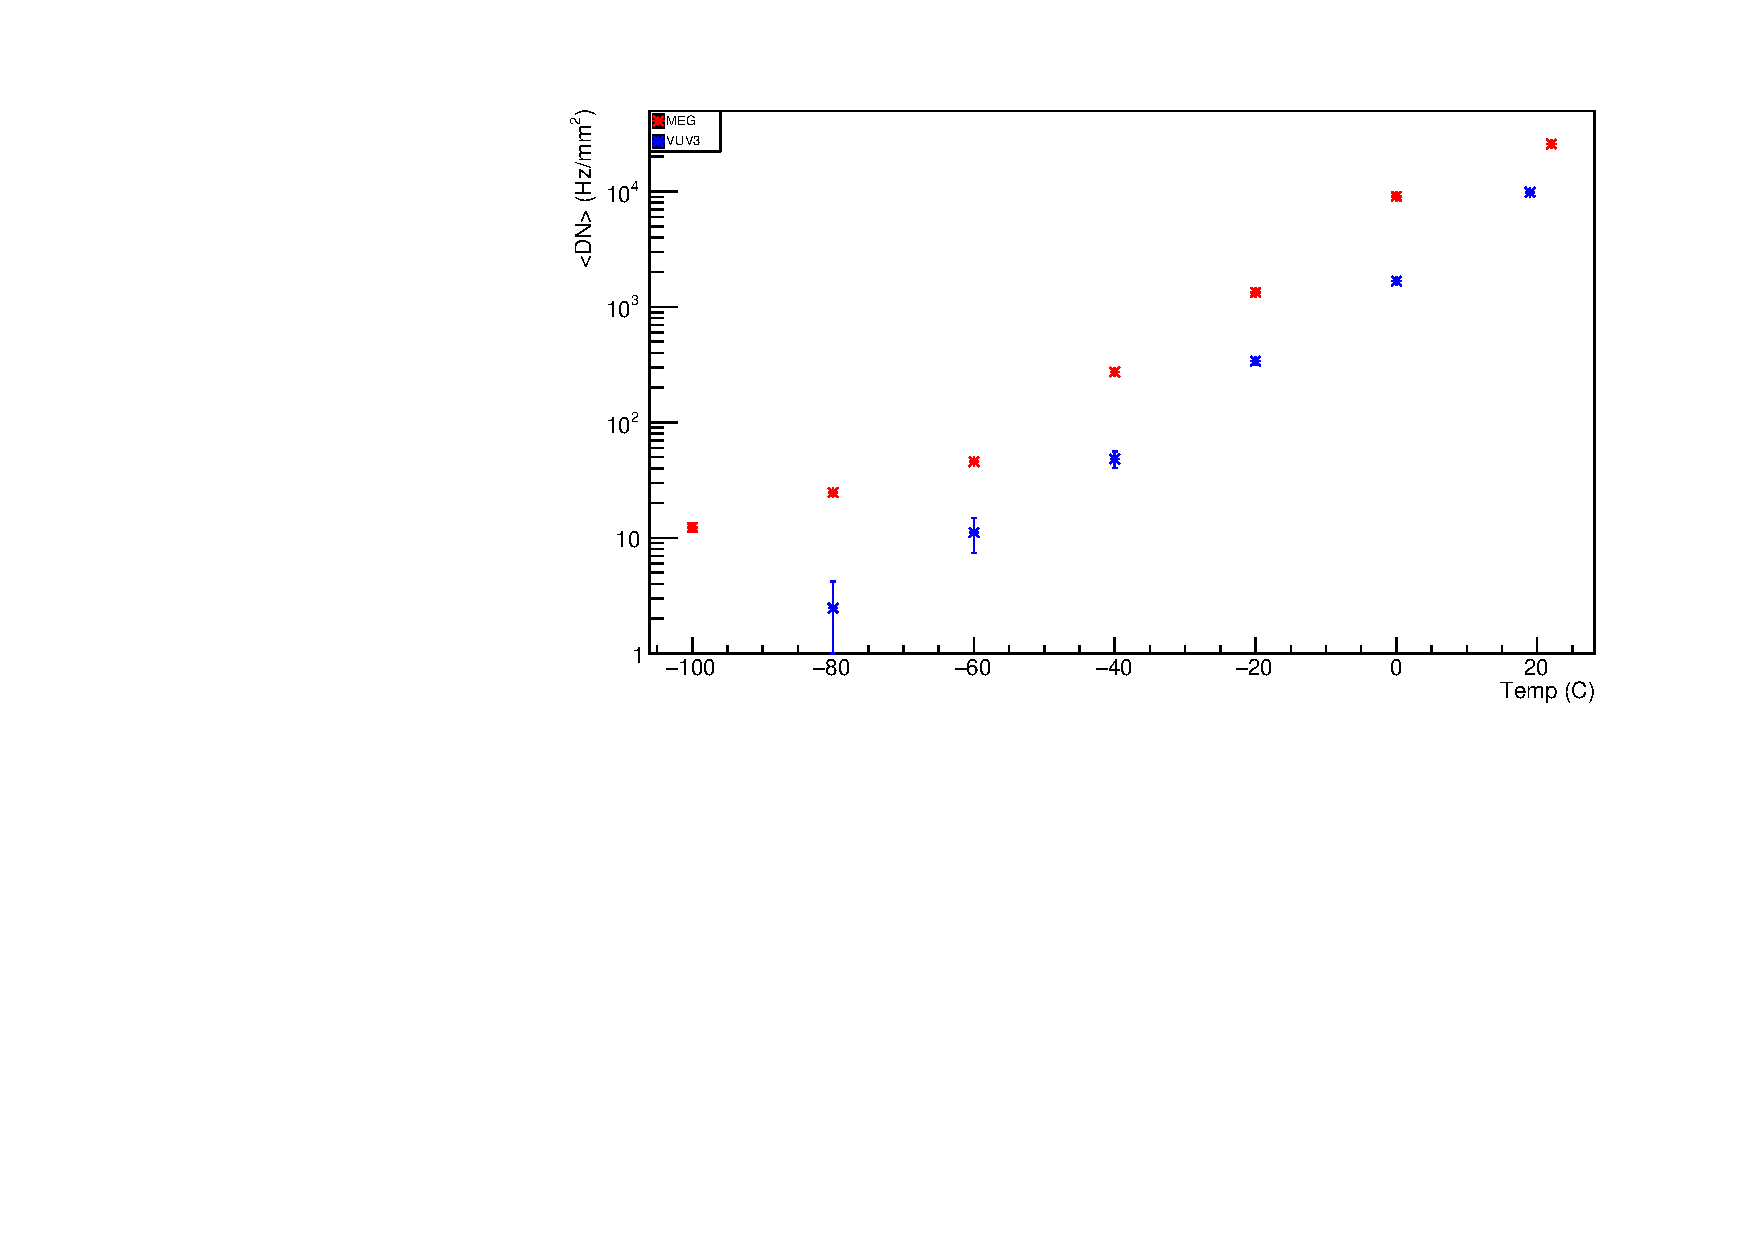
\includegraphics[totalheight=.27\textwidth,trim=0cm 0cm 1.8cm 0.6cm, clip=true]{../Pictures/DNJuly23.pdf}
      \label{fig:DN_vs_temp}}
    \end{subfigure}
  \caption{The breakdown voltage allows working on the same OV for different temperature and thus to plot DN versus temperature.}
  \label{fig:BV_DN_vs_temp}
  \end{figure}
  
  Also as the VUV3 SiPM from HAMMAMATSU seems to be interesting fro nEXO, it is also interesting to plot dark noise rate versus
  over-voltage at $-100^\circ$C. This plot will be compared with the one showing correlated avalanche versus over-voltage at the same 
  temperature for the VUV3. 
  
  \newpage
  
  \begin{figure}[!hbtp]
    \centering
    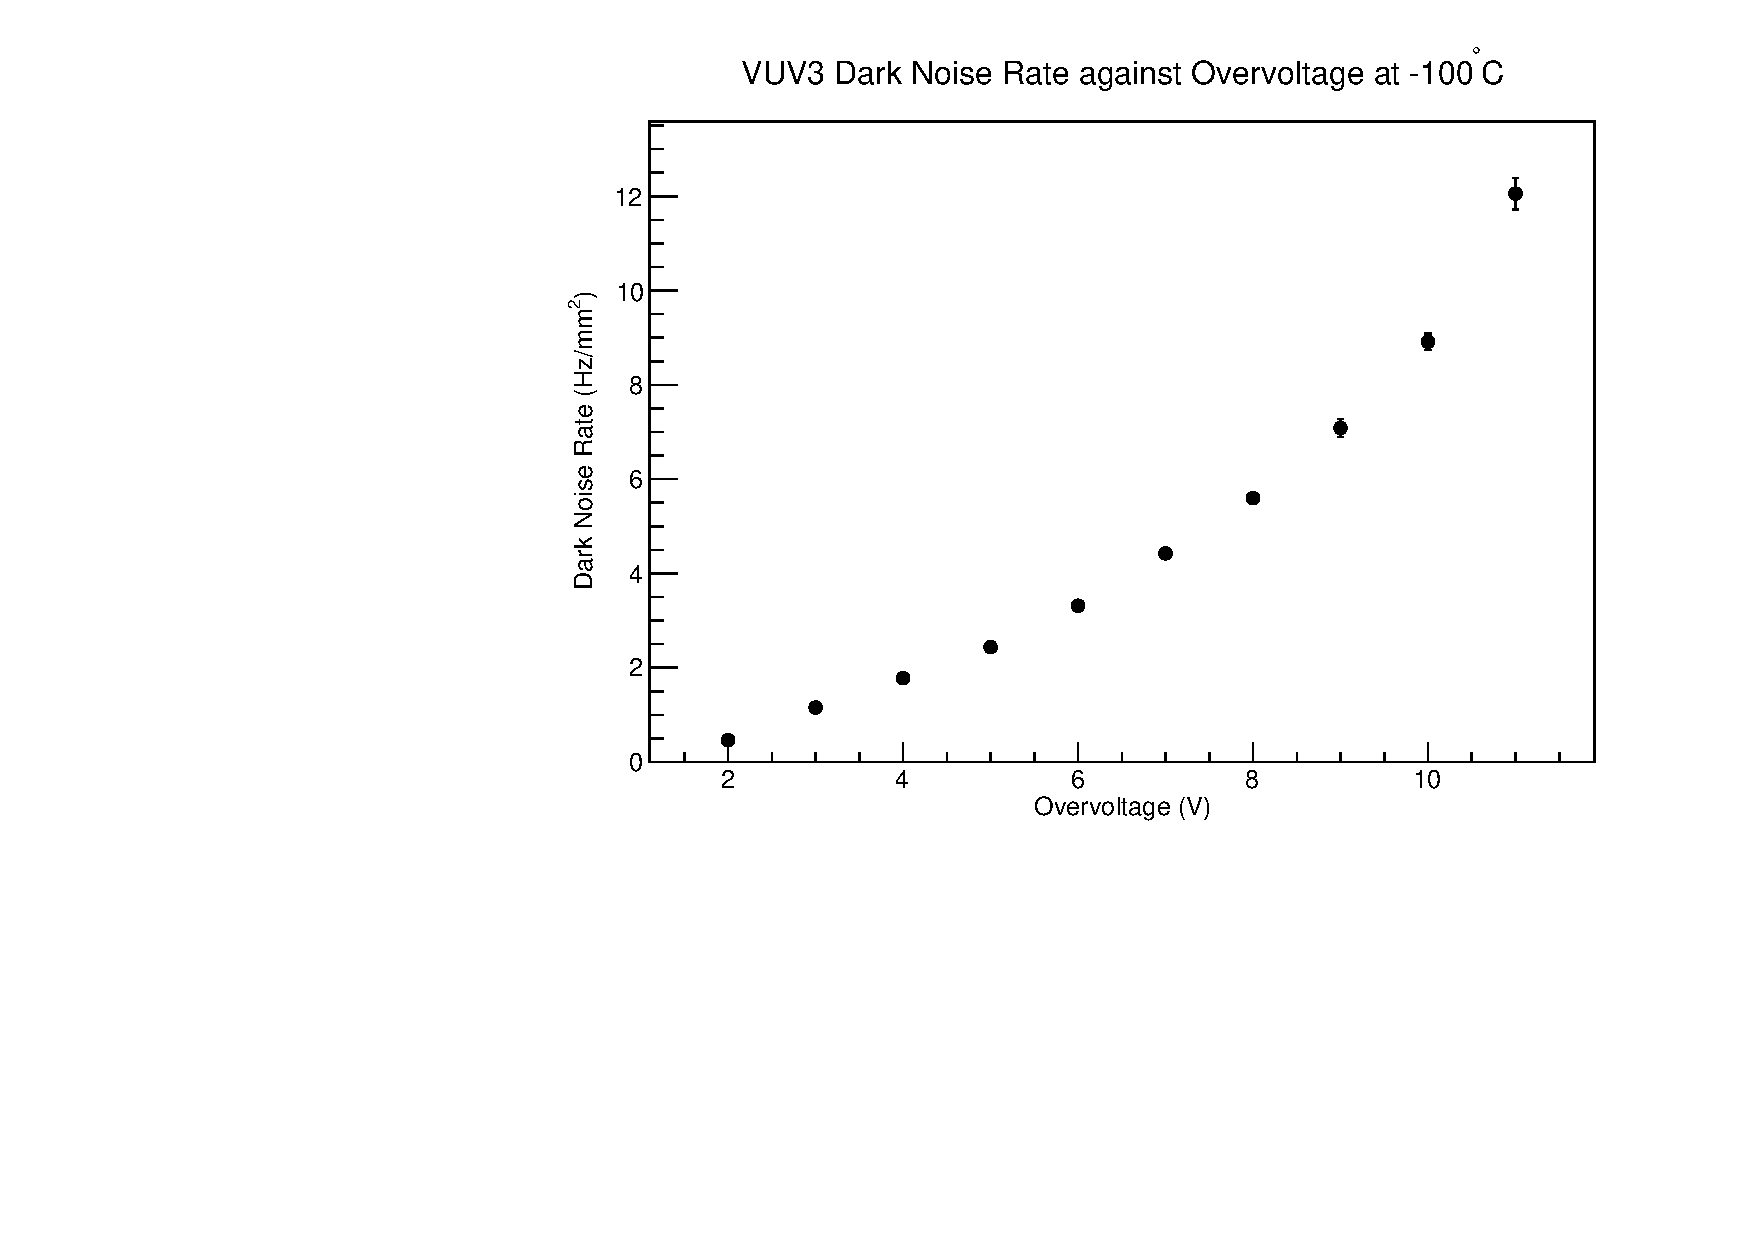
\includegraphics[totalheight=0.5\textwidth,trim=.5cm 0cm 1.8cm 1cm, clip=true]{../Pictures/VUV3_DN_vs_OV.pdf}
    \caption{Dark noise rate increases with the over-voltage applied on the VUV3 SiPM at $-100^\circ$C.}
    \label{fig:DN_vs_OV}
  \end{figure}
  
  \subsection{Analysis: Poisson distribution}
   
  The figure \ref{fig:DN_vs_temp} shows clearly that the dark noise $<DN>$ rate follows a Poisson distribution. 
  The dark noise depends on the temperature: when the temperature increases the number of pulses triggered by hot carriers increases and so 
  the probability 
  of not observing any pulses in the dark region decreases. That means that for a same total number of waveforms, the 0PE peak of 
  the histogram
  \ref{fig:histo_PE} decrease while the other peaks (1PE, 2PE peaks ...) increases. 
  \\
  
  Also the figure \ref{fig:DN_vs_OV} shows that the dark noise dependence on over-voltage is found to be linear up to 7 over-voltage.
  This observation is consistent with previous results shown by nEXO \cite{ref:lloyd_mppc}. 

  \subsection{conclusion}
  
  Compared to the MEG MPPC, the VUV3 SiPM is a good candidate for nEXO. Moreover up to 13 over-voltage \ref{fig:DN_vs_OV}
  the dark noise rate for such a device is still bellow 50 Hz/mm\textsuperscript{2}.
  
  \newpage
  
  \section{Correlated avalanches: CT and AP}\label{sec:correlated}
   
  %Hot carriers in avalanche p-n junction emit photons even in the visible range \footnote{see section}. Thus, 
  %during the avalanche breakdown, a photodiode operating in Geiger mode may emit a few photons. 
  %The photons emitted will be detected by neighboring pixels despite an optical wall between two pixels \footnote{see picture annexe}. 
    
  %It is quiet esay to identify crosstalk on the screen of the scope \footnote{see section, gif orput figure}. 
  %When the height of a peak is double compare to its neighbor, this peak is a cross talk. Physically that means that two avalanche appears and end 
  %on the same time : one comes from the photon coming from a neighboring pixel and the other one comes from the detection of a photon or 
  %reflect dark noise. 
  
  Correlated avalanches refer to crosstalk \ref{subsubsec:CT_section} and after pulse \ref{subsubsec:AP_section}. 
  
  \subsection{Methodology}
  
  \subsubsection{\underline{\textit{Crosstalk}}}
  
  When we trigger on the lamp, histograms from the dark region show the 0PE peak ,1 PE peak, 2PE peak ... where the 0PE peak desn't count
  any pulses,
  the 1PE peak counts single pixel avalanches, the 2PE peak counts pulse shapes triggered from two different pixels ...\\
  When we trigger on the photo-detector, histograms shows the same thing but the previous 0PE peak counts single pixel avalanches
  (and triggered by hot carriers) while the previous ''1PE peak`` counts pulse shapes triggered from two different pixels ...\\
  The second method is more simple than the first one because we know for sure there will always be a pulse shape since the oscilloscope
  records a waveform if the signal reaches a certain threshold (6 mV/div) below the Gaussian noise.\\
  Moreover we managed to make appear each waveform on the middle of the oscilloscope.
  \\
  
  The average number of crosstalk $<CT>$ could be calculated assuming that: 
  
  \begin{equation}\label{eq:CT}
    <CT> = -\ln(\frac{N_{1PE}}{N_{>1PE}}),
  \end{equation}
  
  where $N_{1PE}$ matches with the 1PE peak of the previous histogram and $N_{>PE}$ is calculated by integrating that whole 
  histogram from the beginning of the 1PE peak.\\ 
  When the over-voltage increases, the 1PE peak decreases while all other peaks increase. 
  
  After triggering on the photo-detector, a C++ code ''fillNtp.exe`` smooths a waveform, sets a window size of of 200ns 
  (100ns before and 100ns after) on the middle of a waveform \footnote{The middle is 5$\Pmu$s since each waveform lasts 10$\Pmu$s.}
  and records the minimum of that waveform in a histogram. 
  
  Here is an example of line command: \textit{bin/fillNtp.exe -r 1605 -s 10 -w 200 -b 4900},
  with ''-r, -s, -b`` are described in section \ref{sec:PE}.
  
  \subsubsection{\underline{\textit{Afterpulse}}}
  
  A C++ code called ''pulsefinding.exe`` finds after pulses. This reference \cite{ref:charac_SiPM_nEXO} from \TR gives some explanations 
  and results. 
  
  A certain number of waveforms (15000 in that case) is recorded. The amplitude and the time of the first pulse shape
  of the first waveform (among 15000) are recorded. Then the amplitude and the time of each pulse shape for all the waveform are 
  recorded. 
  Pulse shapes could match with pulse shapes from crosstalk \ref{subsubsec:CT_section}, or from dark noise 
  \ref{subsubsec:DN_photon_shape} or from after pulses \ref{subsubsec:AP_section}.
  \\
  
  In the last case, it is quiet difficult to identify after pulses since they can appear at least 10ns after a primary peak 
  \ref{fig:DN_AP_CT} (A primary peak generates after pulses). To discriminate 
  after pulses from Gaussian noise a common solution is to fit each pulse as describe in that paper \cite{ref:charac_SiPM_nEXO}.
  The drawback of fitting a waveform is the time of operating such code.\\
  The C++ code called ''pulsfinding.exe`` do not fit a waveform since pulse shapes from VUV3 SiPM or from MPPC MEG since they 
  are quiet recognizable (large fall time).\\
  Here is the algorithm of that code:
  
  \begin{itemize}
   \item Scan a waveform
   \item Calculate the standard deviation of the baseline and set a threshold at 4.5 baseline,  
   \item Find a primary peak and record time ($Time_{max}$)and absolute amplitude ($Amp_{max}$),
   \item Find all local maxima around a primary peak,  time ($Time_{max}$) and absolute amplitude ($Amp_{max}$) , 
   \item Check 6 ns before and 1 ns after a local maximum, 
   \item Record time ($Time_{ap}$) and relative amplitude ($Amp_{ap}$) from that local maxmum, 
   \item Calculate the ratio $R$ to discriminate after pulse from Gaussian noise fluctuation:
	 \begin{equation}
	  R = \frac{Amp_{ap}}{Amp_{max}}*\ln(Time_{max}-Time_{ap}) 
	 \end{equation}
   \item Record time and absolute amplitude of that local maximum. 
  \end{itemize}
  
  The picture below will complete the previous explanation:
  
  \begin{figure}[!hbtp]
  \centering 
  \begin{tikzpicture}[scale = 1]%, show background rectangle]
    \draw(0,0) rectangle (11,5);%(x,y)
    %oder has importance 
    
    %pulse shapes and AP
    \draw[-, black, line width=1pt] (0,1)--(3,1);
    \draw[-, black, line width=1pt] (3,1)--(3.8,4);
    \draw[-, black, line width=1pt] (3.8,4)--(5,3);
    \draw[-, black, line width=1pt] (5,3)--(5.3,3.5);
    \draw[-, black, line width=1pt] (5.3,3.5)--(7.3,1);
    \draw[-, black, line width=1pt] (7.3,1)--(11,1);
    
    %script
    \node at(10,0.3) {\color{black} $time (ns)$};
    \node at(1.5,4.6) {\color{black} $Amplitude (mV)$};
    \node at(2.5,2.5) {\color{red} $Amp_{max}$};
    \node at(5.7,3.8) {\color{red} $Amp_{ap}$};
    \node at(2.9,0.3) {\color{blue} $Time_{max}$};
    \node at(6.1,0.3) {\color{blue} $Time_{ap}$};
    %\node at(8,4.5) {\color{black} $R = \frac{Ampl_{ap}}{Amp_{max}}\cdot\ln{(Time_{max}-Time_{ap})}$};
    \node at(9.5,1.7) {\color{green} $Threshold$};
    
    %threshold     
    \draw[-, green, line width=1.3pt, dashed] (0,1.45)--(11,1.45);
    
    % amplitude 
    \draw[|, red, line width=1.3pt] (3.8, 1.45)--(3.8,4);
    \draw[|, red, line width=1.3pt] (5,3)--(5,3.5);
    \draw[-, red, line width=1.3pt,dashed] (5,3.5)--(5.3,3.5);
    
    %time
    \draw[|, red, line width=1.3pt, dashed] (3.8, 0)--(3.8,4);
    \draw[|, red, line width=1.3pt, dashed] (5.3,0)--(5.3,3.5);
    
    
    
  \end{tikzpicture}    
  \caption{The shematic algorithm to find after pulses.Pulse shapes are set positive.}
  \label{fig:effect_temp}
  \end{figure}
  
  
  Also we would like to remind that the probability of not observing after pulses ($P_{0AP}$) fellows a Poisson distribution :
  
  \begin{equation} \label{eq:AP_poisson}
    P_{0AP} = \mathrm{e}^{-<AP>},
  \end{equation}

  where $<AP>$ is the average number of after pulses. 
  
  \newpage 
  
  \subsection{Results}
  
  Here is an example of an histogram used for crosstalk. From right to left 1PE, 2EP, 3PE, 4PE, 5PE:
  
  \begin{figure}[!hbtp]
    \centering
    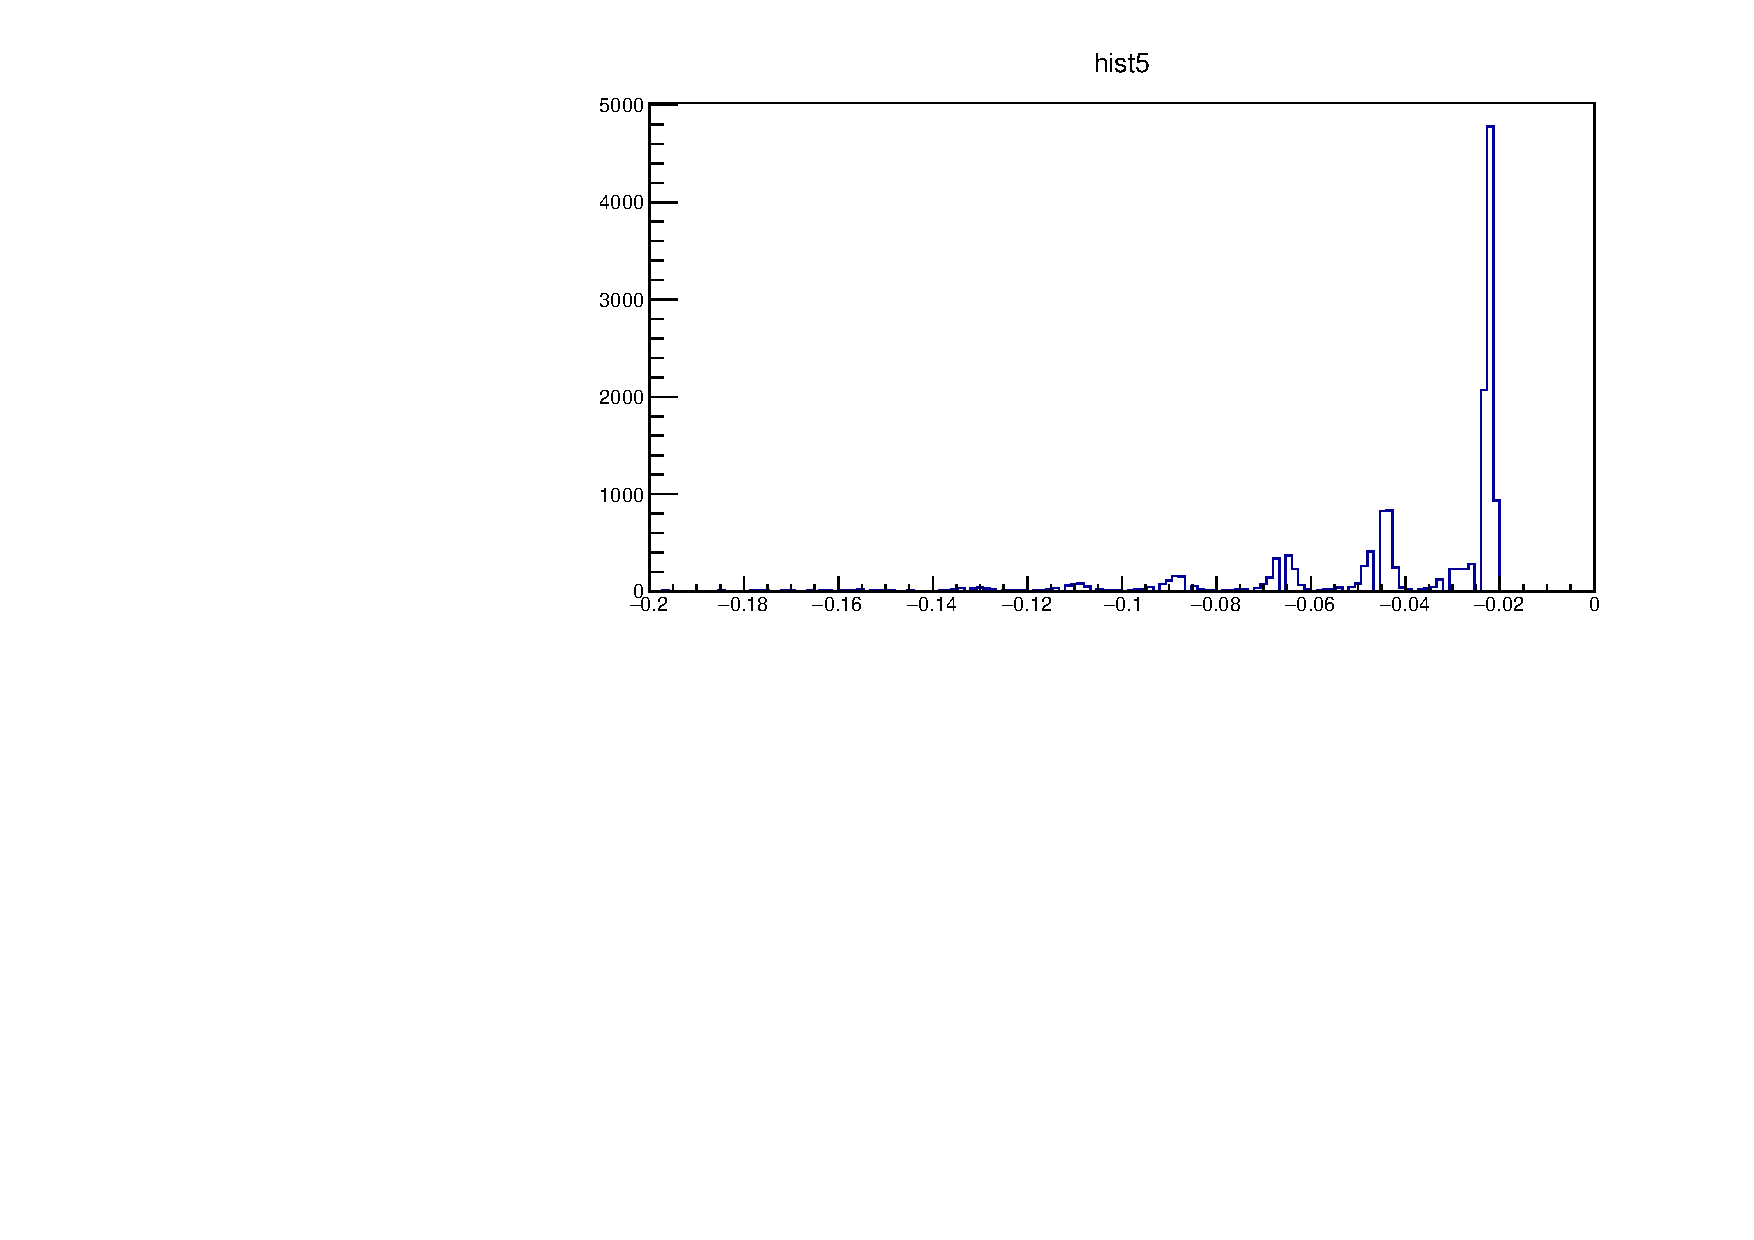
\includegraphics[totalheight=0.4\textwidth,trim=.5cm 0cm 1.8cm 0.9cm, clip=true]{../Pictures/CTHistforTalk.pdf} 
    \caption{An histogram from crosstalk analysis. The device is a VUV3 SiPM at $-100^{\circ}$C at 5 over-voltage.}
    \label{fig:histo_CT}
  \end{figure}
  
  Crosstalk from different devices (coated SiPM, MEG MPPC and VUV3 SiPM) are plotting on the figure below. 

  \begin{figure}[!hbtp]
    \centering
    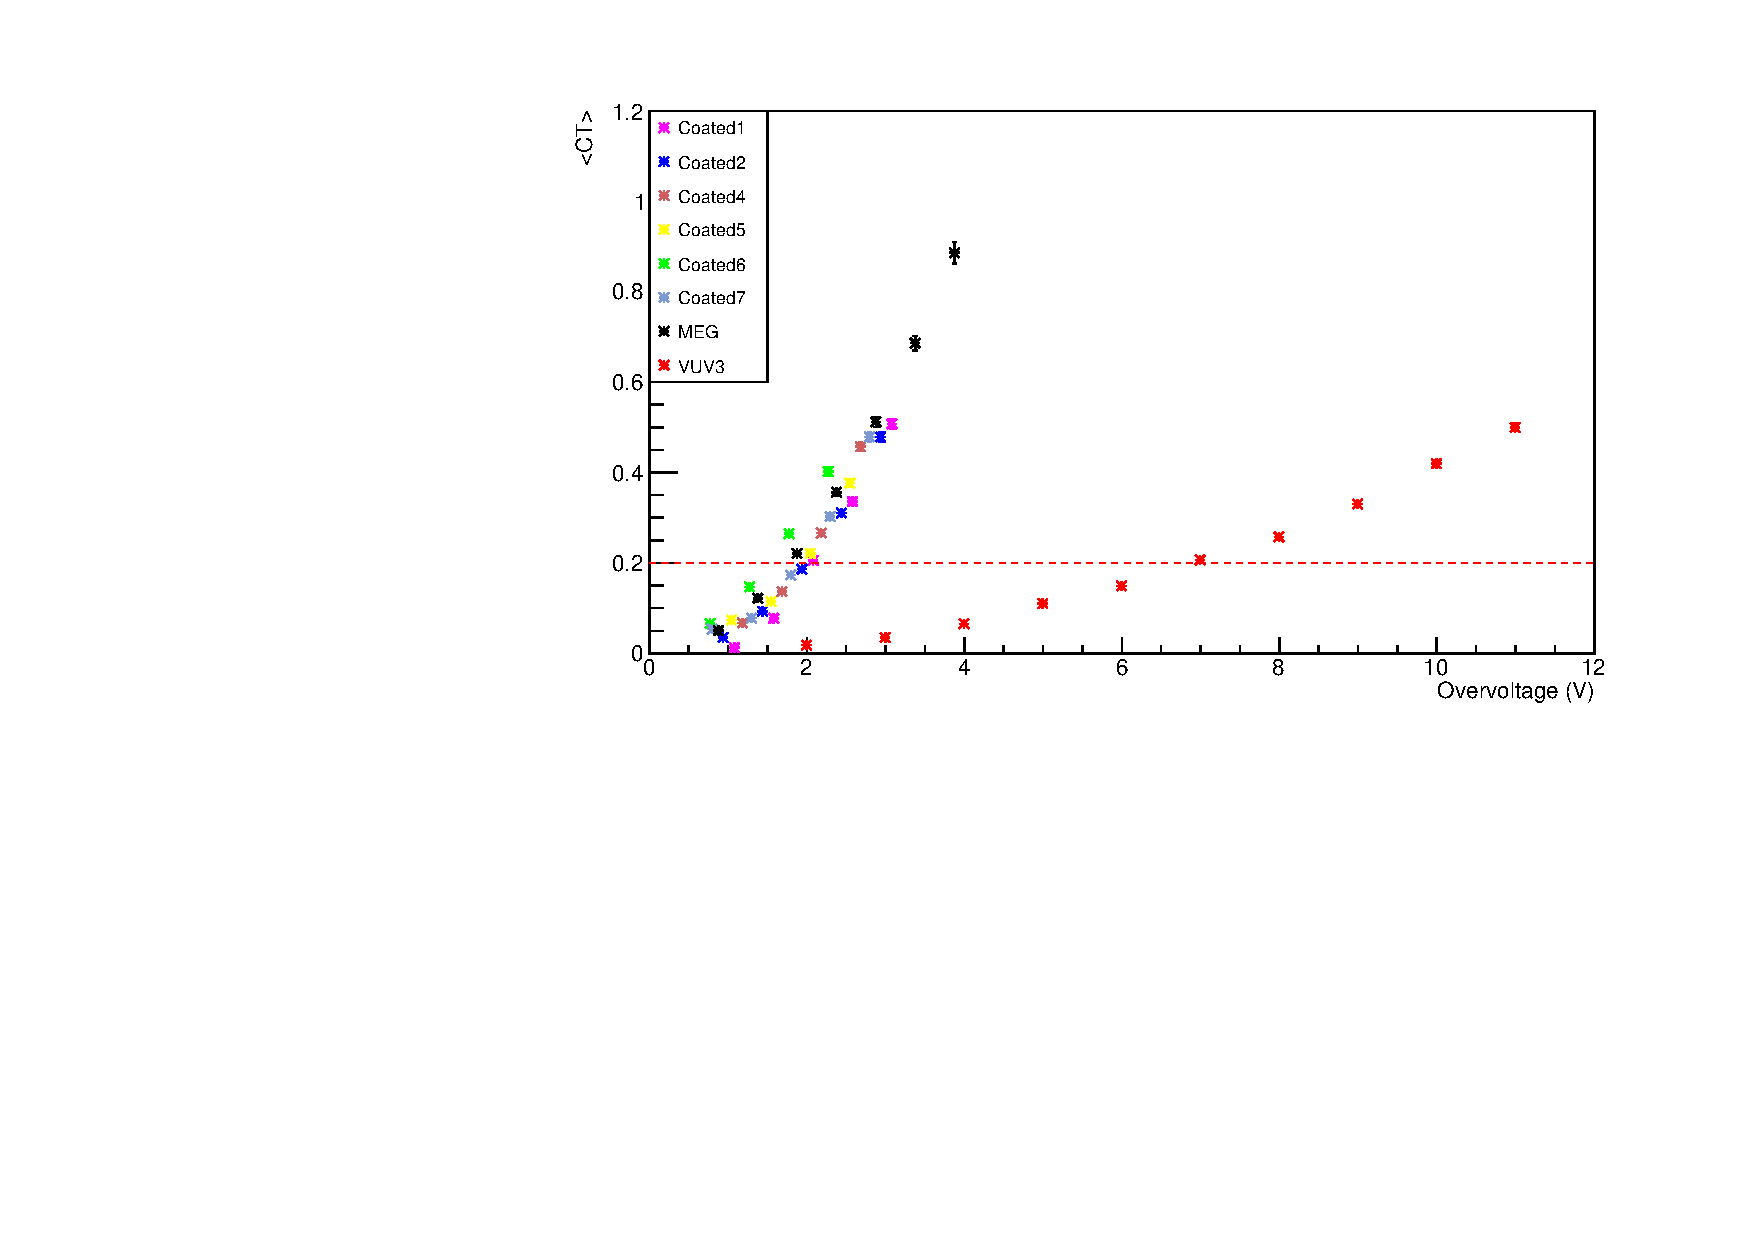
\includegraphics[totalheight=0.5\textwidth,trim=.5cm 0cm 1.8cm 0.9cm, clip=true]{../Pictures/UpdatedVUV3Aug22.pdf}
    \caption{Crosstalk for the VUV3 SiPM reminds below 2 up 6.5 OV.}
    \label{fig:CT}
  \end{figure}
  
  The pulsefinding.exe function allows plotting two different graphs. The first one shows the next pulse probability versus time for different over-voltages
  for the VUV3 SiPM  at $-100^{\circ}$C while the second plot shows the pulse amplitude versus time for the same device at 5 over-voltage at 
  the same temperature:
  
  \newpage
  \begin{figure}[!hbtp]
  \centering
    \begin{subfigure}[Probability of observing next pulses after the first one of the first recorded waveform. Two tails separated
    at 50$\Pmu$s are quiet visible.]{%
      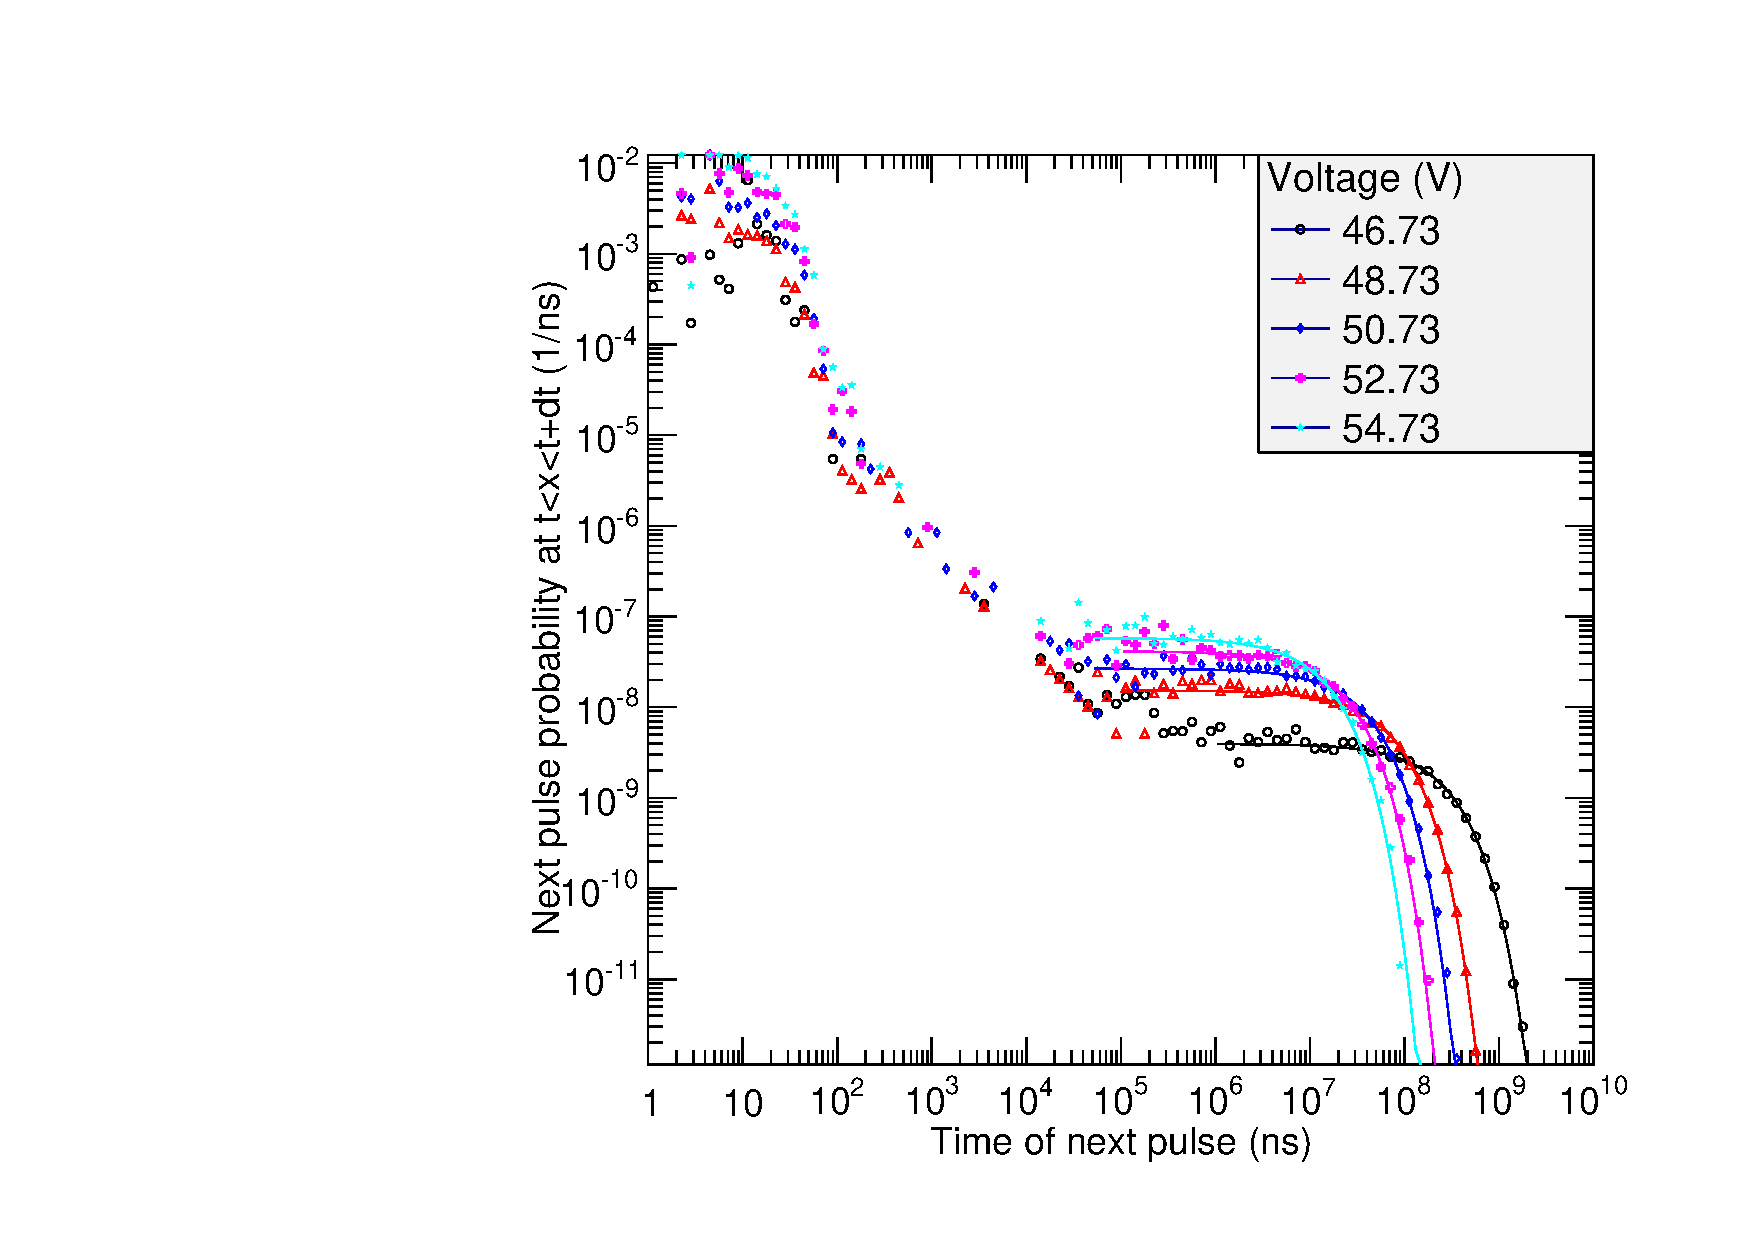
\includegraphics[totalheight=0.47\textwidth,trim=0cm 0cm 1.8cm 0.9cm, clip=true]{../Pictures/deltatime.pdf}
      \label{fig:next_pulse}}
    \end{subfigure}
  \quad  
    \begin{subfigure}[Amplitude of pulses versus time for the VUV3 SiPM.]{%
      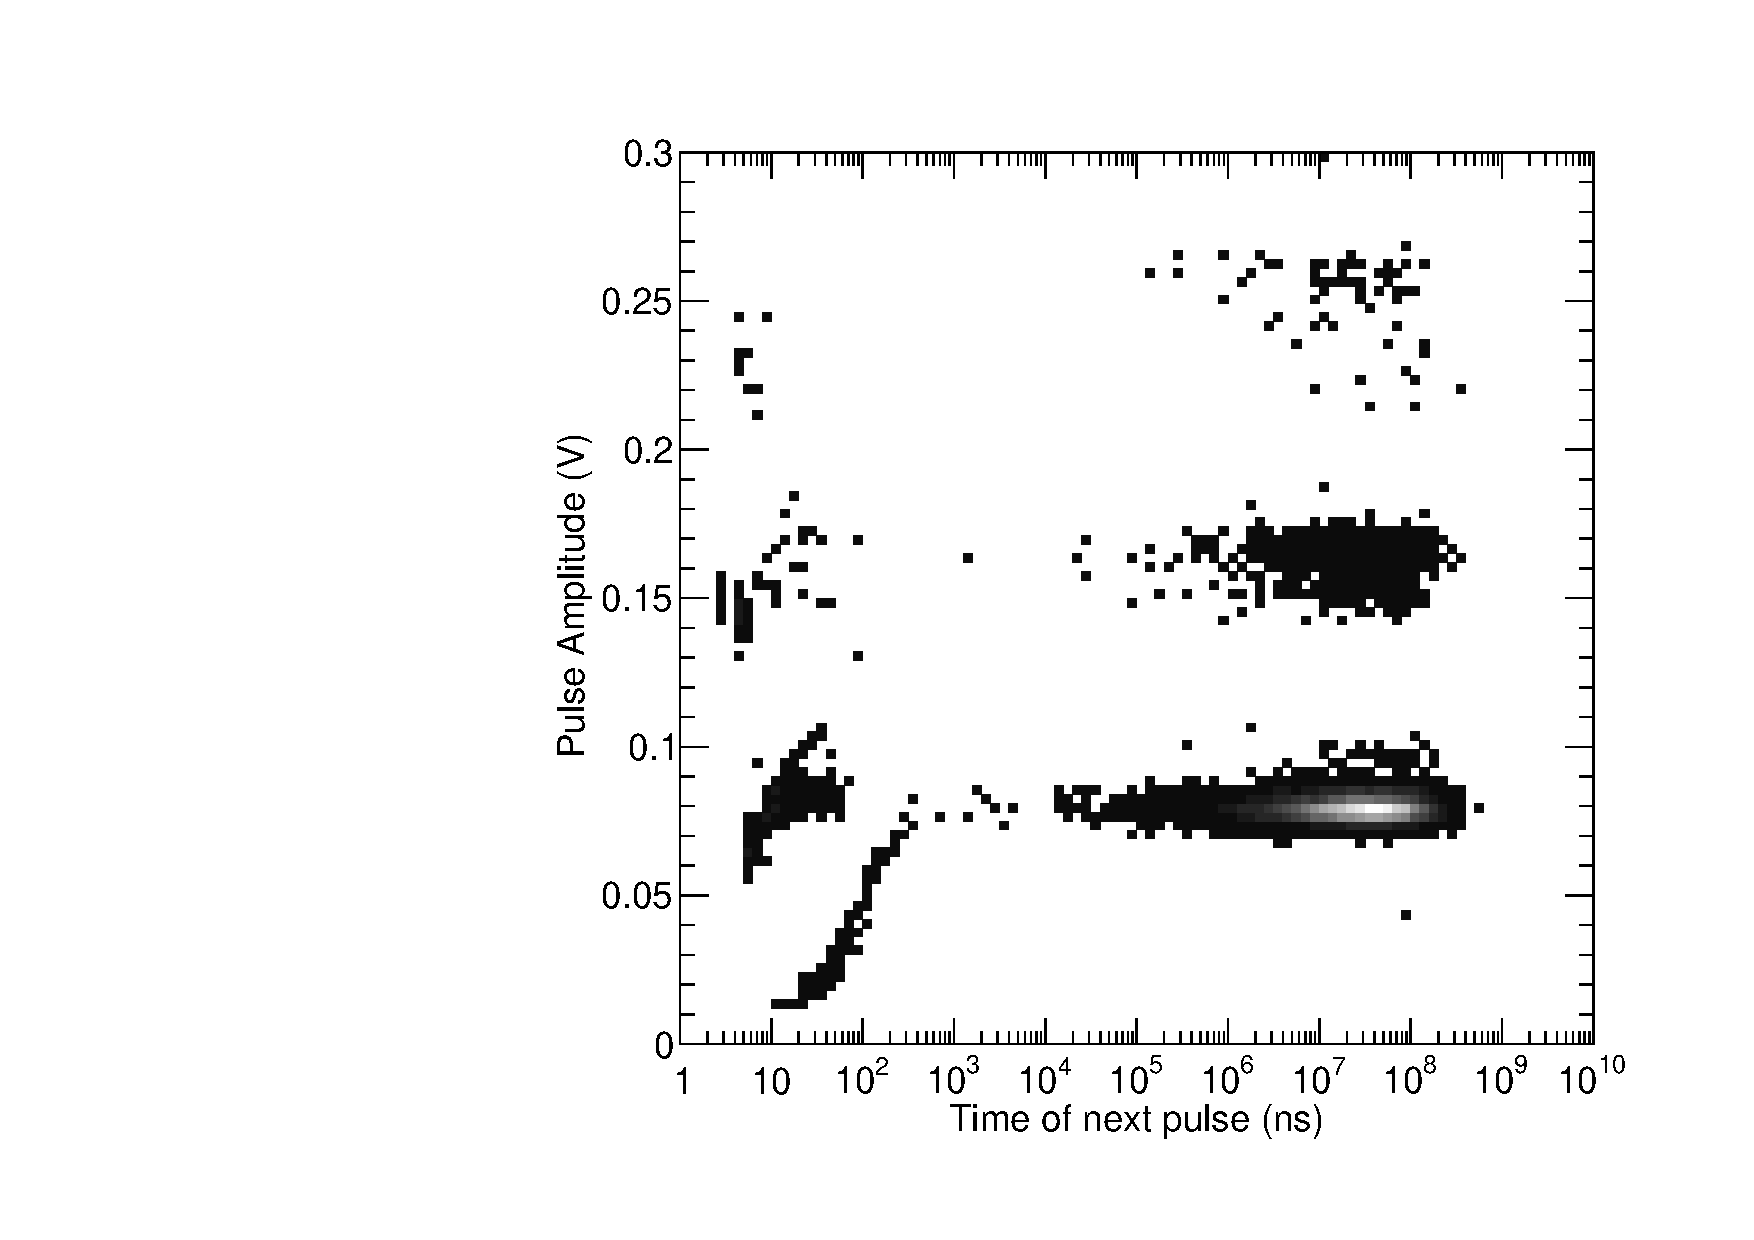
\includegraphics[totalheight=.47\textwidth,trim=0cm 0cm 1.8cm 0.9cm, clip=true]{../Pictures/AmpVUV3_new.pdf}
      \label{fig:pulse_ampl}}
    \end{subfigure}
  \caption{Those two plots are the unique signature of a photo-detector.}
  \label{fig:next_pulse_pulse_ampl}
  \end{figure}
    
  Moreover combining two different methods -fitting and counting- allows plotting the average number of after pulses ($<AP>$) versus over-voltage:
    
  \begin{figure}[!hbtp]
    \centering
    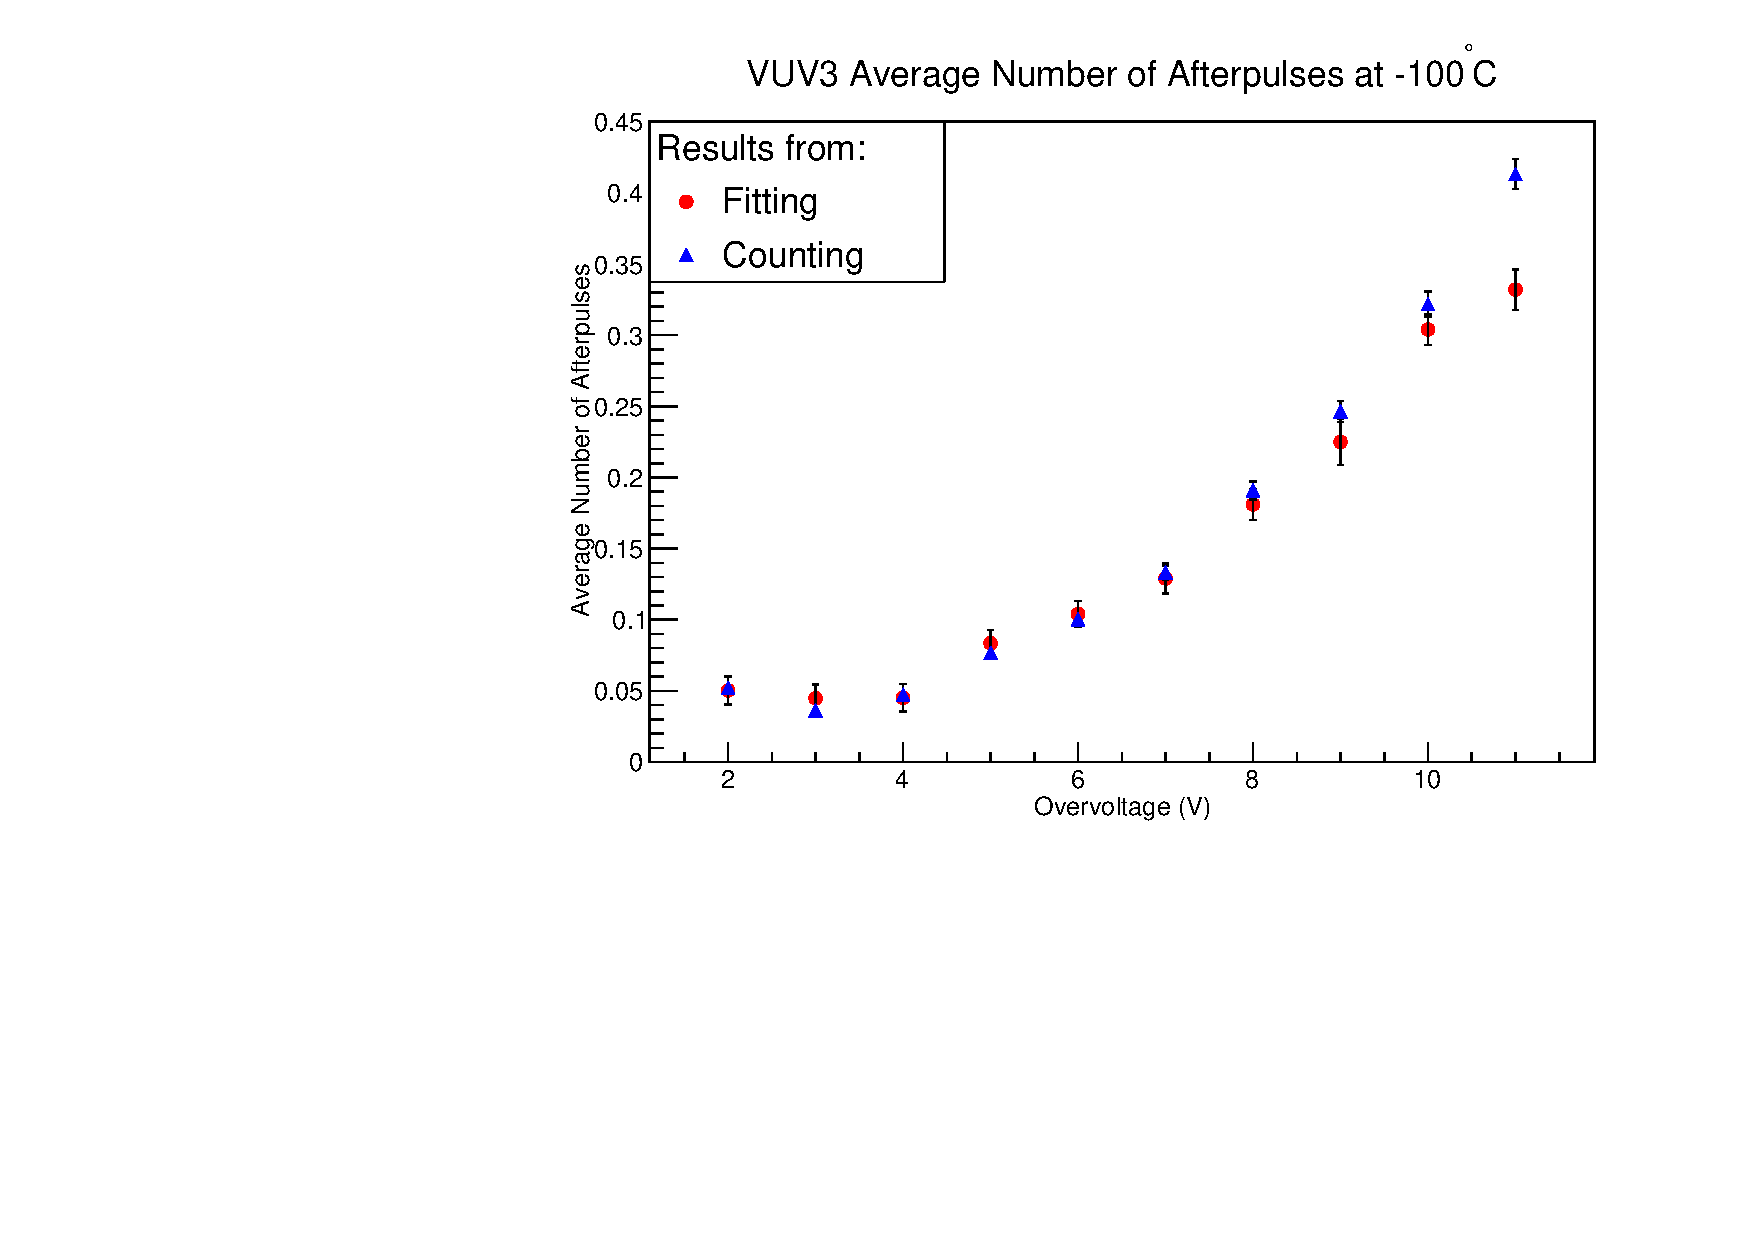
\includegraphics[totalheight=0.55\textwidth,trim=.5cm 0cm 1.8cm 0.9cm, clip=true]{../Pictures/VUV3_AP2_vs_OV.pdf}
    \caption{Average Number of after pulses for the VUV3 SiPM at $-100^{\circ}$C.}
    \label{fig:AP}
  \end{figure}
  
  \newpage
  
  At least adding results from the figure \ref{fig:CT} and from the last figure \ref{fig:AP} allows plotting the average number of correlated 
  avalanches ($<CT> + <AP>$) versus over-voltage:

  \begin{figure}[!hbtp]
    \centering
    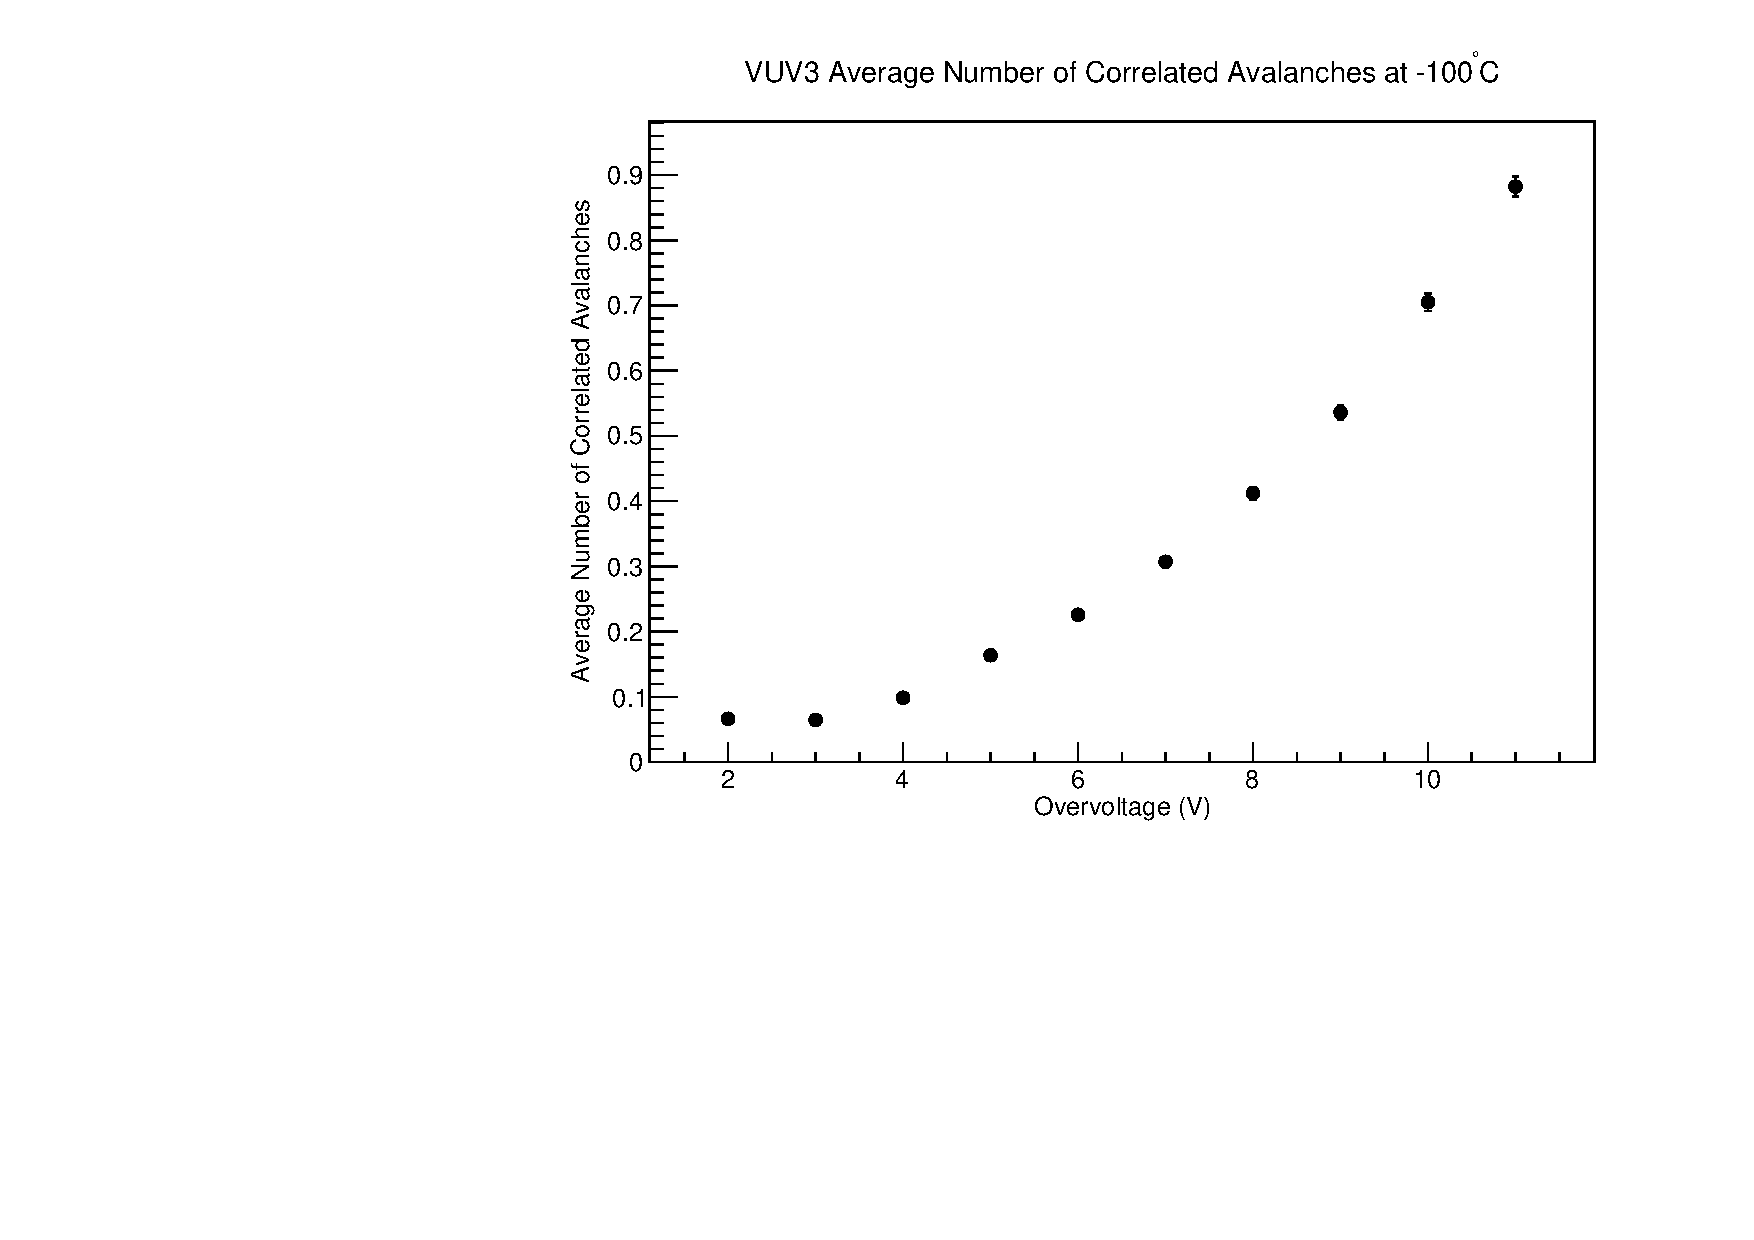
\includegraphics[totalheight=0.55\textwidth,trim=.5cm 0cm 1.8cm 0.9cm, clip=true]{../Pictures/VUV3_CA_vs_OV.pdf}
    \caption{Average Number of Correlated Avalanches for the VUV3 SiPM at $-100^{\circ}$C.}
    \label{fig:CA}
  \end{figure}
  
  \subsection{Analysis}
  
  \subsubsection{\underline{\textit{Crosstalk}}}
  
  CT depends mainly of the over-voltage applied on the photo-detector.\\
  When we increased the voltage applied on the photo-detector, pulse shapes increases. So the number of 2PE peak of the previous 
  histogram increase while the number of 0PE peak decreases for a same number of waveform and thus, the crosstalk increases according 
  the previous relation \ref{eq:CT}.\\
  Moreover the crosstalk for the VUV3 SiPM is 
  very interesting because the average number of crosstalk ($<CT>$) reminds below 0.2 per parent pulse.
  
  \subsubsection{\underline{\textit{After Pulses}}}
  
  The two previous plots side by side \ref{fig:next_pulse_pulse_ampl} are quiet interesting since they characterize a VUV3 SiPM.
  \\
  
  The distribution of the timing difference between consecutive pulses \ref{fig:next_pulse} is used to measure the after pulses and 
  the dark noise rates.
  \\
  
  For measuring after-pulsing rate, the starting pulses are required to correspond to the oscilloscope trigger in order to properly
  account for the oscilloscope dead time. The starting pulses are also required to correspond to single pixel avalanches
  (i.e. triggers with cross-talk are excluded) in order to measure the after-pulsing rate generated by a single parent 
  avalanche.
  On the other hand, the second pulse can have any amplitude (above the noise).\\
  The figure \ref{fig:next_pulse} shows clearly the oscilloscope dead time \footnote{The dead time appears when the 
  oscilloscope is busy to do something else than triggering} because of a sort of cut at 50$\Pmu$s 
  (whatever is the voltage) 
  which separates two different tails.
  \\
  
  That reference from nEXO \cite{ref:charac_SiPM_nEXO} (page 7, equation 1 and 4) helps us to fit the tail after 50$\Pmu$. 
  Here is the equation used:
  
  \begin{equation} \label{eq:fitting_AP_DN}
    P_{total} = P_{0AP}\cdot <DN>\cdot\mathrm{e}^{-<DN>\cdot t},
  \end{equation}

  where $P_{0AP}$, $<DN>$ and t are the probability of observing no after pulse, the dark noise rate (Hz/mm\textsuperscript{2})
  and the 
  time, respectively.\\
  Then $P_{0AP}$ is extracted from that fitting and assuming that the after pulse fellows a Poisson distribution 
  \ref{eq:AP_poisson}, 
  it is possible to calculate the average number of after pulses ($<AP>$) for different voltages. That fitting method shows 
  clearly the $<AP>$ versus over-voltage for the VUV3 SiPM at $-100^{\circ}$C.\\
  Also an algorithm let us count the average number of after pulses. Indeed a ratio is defined : 
  
  \begin{equation} \label{eq:ratio}
    R = \frac{\textrm{number of after pulses}}{\textrm{number of primary peaks}},
  \end{equation}
  
  where the number of primary peaks corresponds to all peaks which are not counting as after pulses since they trigger
  after pulses.\\
  If the time between two consecutive pulses 
  -$\Delta t$- is lower than 50$\Pmu$s and
  upper than 10$\Pmu$s, pulses are considered as after pulses. If that $\Delta t$ is lower than 10$\Pmu$s and 
  if the amplitude of founded
  pulses are upper than 0.5 PE (to avoid Gaussian noise fluctuation), those pulses are crosstalk. Else, all other pulses 
  are counting as after pulses.\\
  The two methods -fitting and counting - match quiet well as we can see it on the figure \ref{fig:AP}.
  \\
  
  For measuring the dark noise, the method is to fit the tail after 50$\Pmu$ since pulses after 50$\Pmu$ are considered as pulses
  triggered by hot carriers. We noticed that after pulses should be generated in a lapse of time before
  50$\Pmu$ and thus, pulses after 50$\Pmu$ can be counted as dark noise.\\
  As well as the number $<AP>$ is deduced from the fitting \ref{eq:fitting_AP_DN}, the dark noise rate $<DN>$ is 
  deduced from the fitting. The figure \ref{fig:next_pulse} shows clearly that the dark noise rate depends of the voltage
  applied on the VUV SiPM (breakdown voltage of 44.73V +/- 0.03 at $-100^{\circ}$C) and allow also plotting the previous figure 
  \ref{fig:DN_vs_OV}. 
  \\
  
  For the distribution of the pulse amplitude versus time, there is no correlation between time and amplitude except below 
  3$\Pmu$s which is the recovery time of a pixel. The recovery time is the amount of time before pulses will be release with their 
  full amplitude.\\
  Physically inside the photo-detector, after an avalanche, the voltage across the diode recovers with a time 
  constant given by the product of the pixel capacitance and quenching resistance. 
  Pulses with high amplitude must come from different pixels (crosstalk) even though they occurred within the recovery time scale. 
  If so the quenching resistor absorbs the created carriers and pulses do not have enough time to release with their full amplitude.\\
  The main band at at $∼80$ mV corresponds to pulses from single pixel avalanches while the other bands corresponds with pulses whose
  amplitude is two or three or more time larger pulse amplitude from the main band. 
  \\
  
  \subsubsection{\underline{\textit{Correlated Avalanche}}}
  
  The last figure \ref{fig:CA} shows the correlated avalanches of the VUV3 SiPM at $-100^\circ$C. Adding the figure \ref{fig:AP} and the figure
  \ref{fig:CT} allows plotting that last figure since the average number of correlated avalanches is the sum of 
  the average number of crosstalk and the average number of after pulses.\\
  The VUV3 SiPM lets us increase the over-voltage up to 5V and the average number of correlated avalanches is still under 0.2 per parent 
  pulse. That means that below 5 over-voltage, the probability of observing correlated avalanche generated by a primary pulse is below 
  20$\%$ \ref{item:conditions}.
  
   
  
%%%%%%%%%%%%%%%%%%%%%%%%%%%%%%%%%%%%%%%%%%%%%%%%%%%%%%%%%%%%
%        chapter 5 summarize about progression             %
%%%%%%%%%%%%%%%%%%%%%%%%%%%%%%%%%%%%%%%%%%%%%%%%%%%%%%%%%%%%

\chapter{Synthesis}

  One of the main goal of this internship was to calculate the efficiency for different photo-detectors (MEG MPPC, SiPM, coated 
  SiPM, FBK ...).\\
  Nevertheless we noticed that our results for the VUV3 SiPM are not reproducible. In oder to understand what is(are) the source(s) of 
  that non reproducibility, we tried to eliminating different parameters such as the position and the voltage of the lamp, the quantity 
  of oxygen inside the box and some dust on the sensitive area of the photo-detectors.\\  
  We arrived at the conclusion that the misalignment of the narrow beam with the collimator on the top and on the bottom may be the main 
  source of our problem.\\
  Moreover working at $-100^\circ$C seems to influence the position of the board holding the two collimators, the beam splitter and the 
  photo-detector on the top: after three hours of cooling, the efficiency of the photo-detector on the top increases while the efficiency 
  of the one on the bottom decreases. Nevertheless both of them seems to reach a sort of plateau which allow making a temporary comparison 
  between the MEG MPPC and the VUV3 SiPM at $-100^\circ$C (assuming that the beam reminds constant).
  
  \paragraph{\textit{Recommendations }}
  
  We recommend to the next students to enlarge the beam with a divergent lens. So that the beam could always reach the hole of 1 mm of 
  the collimator even tough the board is moving down while cooling at very low temperature.
    
  On the contrary results about dark noise and correlated avalanches are confident, especially for the VUV3 SiPM which fulfills the last two
  requirements for nEXO:
  
  \begin{itemize}
   \item Its dark noise rate is less than 3 Hz/mm\textsuperscript{2} for an over-voltage of 5V at $-100^\circ$C 
   \footnote{It is required 50 Hz/mm\textsuperscript{2} for such a temperature.}.
   \item Its average number of correlated avalanches is less than 0.2 per parent pulses for the same over-voltage at the same working 
   temperature \footnote{It is required 0.2 per parent pulses in the same conditions.}.
  \end{itemize}

  \paragraph{\textit{Recommendations }}
  We also recommend to the next students to confirm such results for the MEG MPPC and the coated SiPM \ref{fig:table_SiPM}.\\  
  At least some investigations need to be done about the attenuation of light as described in appendix \ref{app:tests}.
  
%%%%%%%%%%%%%%%%%%%%%%%%%%%%%%%%%%%%%%%%%%%%%%%%%%%%%%%%%%%%
%        chapter 6 summarize about progression             %
%%%%%%%%%%%%%%%%%%%%%%%%%%%%%%%%%%%%%%%%%%%%%%%%%%%%%%%%%%%%

\chapter{Professional assessments} 

  This internship has been very beneficial and I found it very interesting. I learned a lot from my co-workers about SiPMs. 
  Their knowledges on such a subject let me improve my scientific and rigorous thinking in physics. 
  I have always solicited them when I was fighting with some difficulties.
  \\
  
  I was happy to use my theoretical knowledges about electronics, matter physics and 
  physics about detectors. I also improved my engineering thinking by trying 
  to adopt practical solutions for all issues we had.  
  \\
  
   
  
%%%%%%%%%%%%%%%%%%%%%%%%%%%%%%%%%%%%%%%%%%%%%%%%%%%%%%%%%%%%
%        chapter 7 summarize about progression             %
%%%%%%%%%%%%%%%%%%%%%%%%%%%%%%%%%%%%%%%%%%%%%%%%%%%%%%%%%%%%

\chapter{Human impact}

  I really enjoyed working at TRIUMF and also working in an English environment. 
  From the beginning of my internship I tried to improve my English skills in oder
  to improve my knowledges on the subject. The natural open minding of the Canadian
  help me for that. 
  \\
  
  I also enjoyed working in a laboratory on a research internship. Having good and new results, with a possible publication at the 
  end, was one of my motivations at work. I also enjoyed working on that internship with a a difficulty linked to a research subject.\\
  I also enjoyed working with autonomous and flexible hours.\\
  I enjoyed that internship because I was asked to use my theoretical knowledges to explain physical phenomena. 
  

%%%%%%%%%%%%%%%%%%%%%%%%%%%%%%%%%%%%%%%%%%%%%%%%%%%%%%%%%%%%
%        chapter 8 summarize about progression             %
%%%%%%%%%%%%%%%%%%%%%%%%%%%%%%%%%%%%%%%%%%%%%%%%%%%%%%%%%%%%

\chapter{Conclusion}
  
  This internship ends my engineering study at \TPS. This has been a very good experience which allow taking 
  responsibilities in nEXO's collaboration.
  \\
  
  My internship was a very interesting technological subject. I have been asked to 
  use the two different parts of my engineering and scientific courses
  I could also discover working in a team for a hug collaboration. 
  
  As far as possible my work contributed to make some progress on the study of SiPMs. 
  Results are quiet positive and put forward my engineering formation. 
  
  
%%%%%%%%%%%%%%%%%%%%%%%%%%%%%%%%%%%%%%%%%%%%%%%%%%%%%%%%%%%%
%                   bibliography                           %
%%%%%%%%%%%%%%%%%%%%%%%%%%%%%%%%%%%%%%%%%%%%%%%%%%%%%%%%%%%%
\begin{thebibliography}{999}
  \bibitem{ref:modern_particle_physics} Mark Thomson, \textit{Modern Particle Physics}, Hardcover,\textbf{Oct 21, 2013}.
  \bibitem{ref:fondamental_statistical_and_thermal_physics} Frederick Reif, \textit{Fundamentals of Statistical and Thermal Physics}, 
  Hardcover, \textbf{Jan 6, 2009}.
  \bibitem{ref:majorana_fermions} \url{https://en.wikipedia.org/wiki/Majorana_fermion}.
  \bibitem{ref:motivation_and_introduction} \textit{Scintillation light detection in nEXO}, \textbf{May 13, 2015}.
  \bibitem{ref:mppc_hammamatsu} \url{http://www.hamamatsu.com/us/en/community/optical_sensors/tutorials/physics_of_mppc/index.html?utm_source=googleplus&utm_medium=social&utm_campaign=hc-social}.
  \bibitem{ref:\xfl} \url{www.hamamatsu.com/resources/pdf/etd/Xe-F_TLS1003E.pdf}, page 4, Flash Pulse Waveform.
  \bibitem{ref:PN_junction_ref} \url{https://en.wikipedia.org/wiki/P$\%$E2$\%$80$\%$93n_junction}.
  \bibitem{ref:Hammamatsu_pn_junction} Kenneth R. Spring and Michael W. Davidson, \textit{Avalanche Photodiodes}, available at \url{http://hamamatsu.magnet.fsu.edu/articles/avalanche.html}.
  \bibitem{ref:mppc_meg} \textit{MPPC and MPPCC module for precision measuremnts}, HAMMAMATSU, \textbf{May 13, 2015}, page 2, figure 2.
  \bibitem{ref:charac_SiPM_nEXO} I. Ostrovskiy et al., \textit{Characterization of Silicon Photomultipliers for nEXO}, arXiv:1502.07837v2 [physics.ins-det], \textbf{Jul 6, 2015}
  \bibitem{ref:charac_SiPM} Patrick Eckert et al., \textit{Characterisation studies of silicon photomultipliers}, available at \url{http://arxiv.org/abs/1003.6071}, \textbf{2010}.
  \bibitem{ref:phelham_filter} \url{http://www.teo.com.cn/filespath/files/20130802133536.pdf}, page 4, figure Phelham Research Opticall L.L.C Narrowband Filter P/N:172-NB Filter.
  \bibitem{ref:lloyd_mppc} Pierre-Andr'e Amaudruz et al., \textit{Pixelated Geiger-Mode Avalanche Photo-Diode Characterization through Dark Current Measurement}, arXiv:1312.0545 [physics.ins-det], \textbf{Dec 2, 2013}.
\end{thebibliography}


%%%%%%%%%%%%%%%%%%%%%%%%%%%%%%%%%%%%%%%%%%%%%%%%%%%%%%%%%%%
%                    appendix                              %
%%%%%%%%%%%%%%%%%%%%%%%%%%%%%%%%%%%%%%%%%%%%%%%%%%%%%%%%%%%%
\appendix

\chapter{Terminology}\label{anx:terminology}
  
  \begin{tabular}{|c|c|}
    \hline
    \bf Acronym & \bf Meaning\\
    \hline
    \hline
    EXO & Enriched Xenon Observatory\\
    \hline
    nEXO & next generation Enriched Xenon Observatory\\
    \hline
    SiPM & Silicum Photo Multiplier\\
    \hline
    MPPC & Multi-Pixel Photon Counter\\
    \hline
    VUV & Ultra Vacuum \\
    \hline
    APD & Avalanche Photo-diode \\
    \hline
    BV & Breakdown Voltage \\
    \hline
    OV & Over Voltage\\
    \hline
    DN & Dark Noise\\
    \hline
    CT & Crosstalk \\
    \hline
    PE & Photon Electron \\
    \hline
    \hline
  \end{tabular}


%%%%%%%%%%%%%%%%%%%%%%%%%%%%%%%%%%%%%%%%%%%%%%%%%%%%%%%%%%%%
%                    appendix : nEXO                       %
%%%%%%%%%%%%%%%%%%%%%%%%%%%%%%%%%%%%%%%%%%%%%%%%%%%%%%%%%%%%

\chapter{Details about the setup}\label{app:setup}

  \section{Pictures of the setup}
  
  Here is a general picture of the setup. The table below the figure explains the number. 
  
  \begin{figure}[!hbtp]
      \centering
      \begin{tikzpicture}
      \node (img) {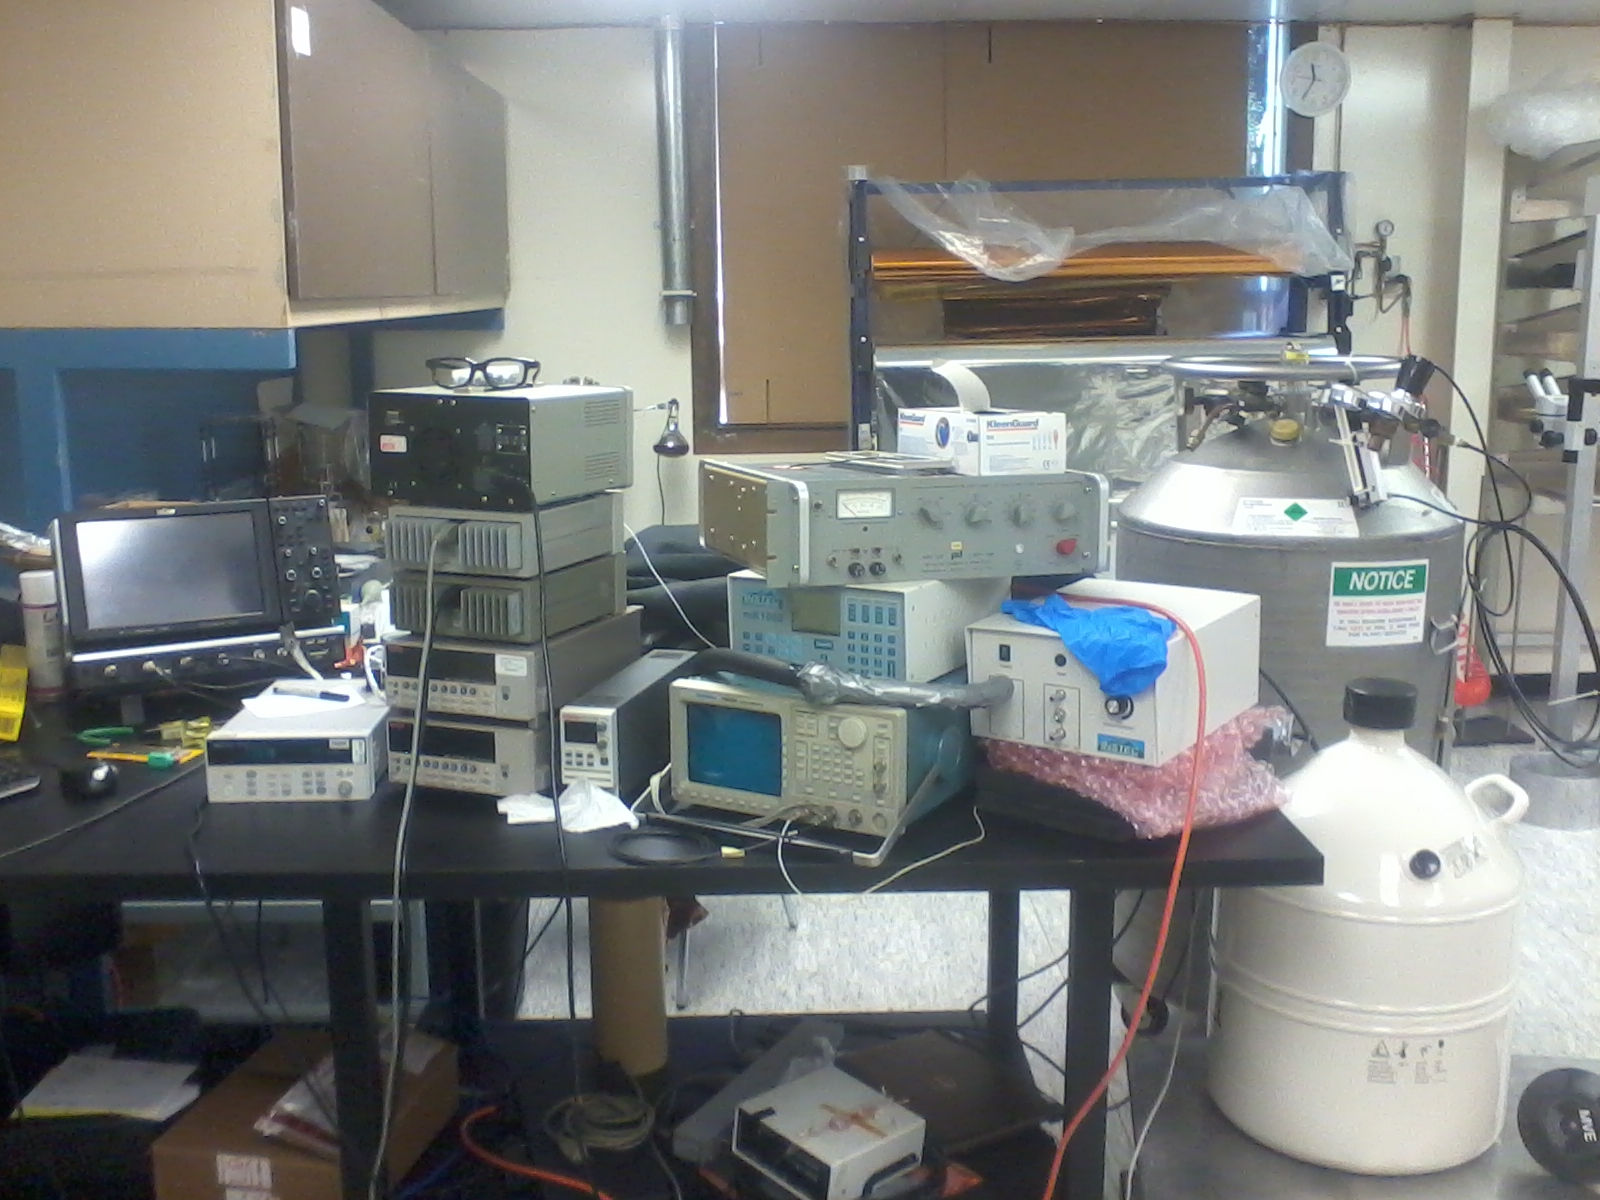
\includegraphics[width=.8\textwidth,trim=0cm 0cm 0cm 0cm, clip=true]{../Pictures/Pictures_Setup/general_picture.jpg}};
      \tikzstyle{every node} = [circle, fill = green, scale = .8]
      \node  at ( -17mm,13mm) {\color{black} \textbf{$1$}};
      \node  at ( -24mm,4mm) {\color{black} \textbf{$2$}};
      \node  at ( -27mm,-2mm) {\color{black} \textbf{$3$}};
      \node  at ( -24mm,-7mm) {\color{black} \textbf{$4$}};
      \node  at ( -27mm,-12mm) {\color{black} \textbf{$5$}};
      \node  at ( -42mm,-13.5mm) {\color{black} \textbf{$6$}};
      \node  at ( 0mm,-13.5mm) {\color{black} \textbf{$7$}};
      \node  at ( 6mm,5mm) {\color{black} \textbf{$8$}};
      \node  at ( 1mm,-2mm) {\color{black} \textbf{$9$}};
      \node  at ( 20mm,-8mm) {\color{black} \textbf{$10$}};
      \node  at ( 47mm,-20mm) {\color{black} \textbf{$11$}};
      \node  at ( 45mm,1.5mm) {\color{black} \textbf{$12$}};
      \node  at ( -50mm,1mm) {\color{black} \textbf{$13$}};
      \end{tikzpicture}
      \caption{General pictures of the setup.}
      \label{fig:general_picture}
  \end{figure}
  
  \newpage
  
  Here is the meaning of each number:
  
  \begin{figure}[!hbtp]
  \centering
  \begin{tabular}{|c|c|}
    \hline
    \bf Numbers & \bf Meaning \\
    \hline
    \hline
    1 & Set the voltage to the lamp  \\\hline
    2 & Set the voltage of 12 V for both amplifiers  \\\hline
    3 & Set volatge of 5 V to control device number 4,5,6 from a computer  \\\hline
    4 & Set voltage of the photodetector on the bottom  \\\hline
    5 & Set voltage of the photodetector on the top  \\\hline
    6 & Display and Record temperature from all sensors \\\hline
    7 & Set the trigger of the lamp \\\hline
    8 & Set the voltage for a PMT \\\hline
    9 & Set temperature to cool down the photodetector on the bottom  \\\hline
    10 & Allow cooling down  \\\hline
    11 & Small bottle whose N2 is used to cool down the photodetector \\\hline
    12 & Big bottle to fille the box with N2  \\\hline      
      13 & Oscilloscope allowing displaying and registering waveforms \\
    \hline
    \hline
  \end{tabular}
  \caption{Different devices used for the setup.}
  \label{fig:table_SiPM}
  \end{figure}
  
  To reduce light leaks from the  \xfl, a black box covers the lamp:
  
  \begin{figure}[!hbtp]
    \centering
    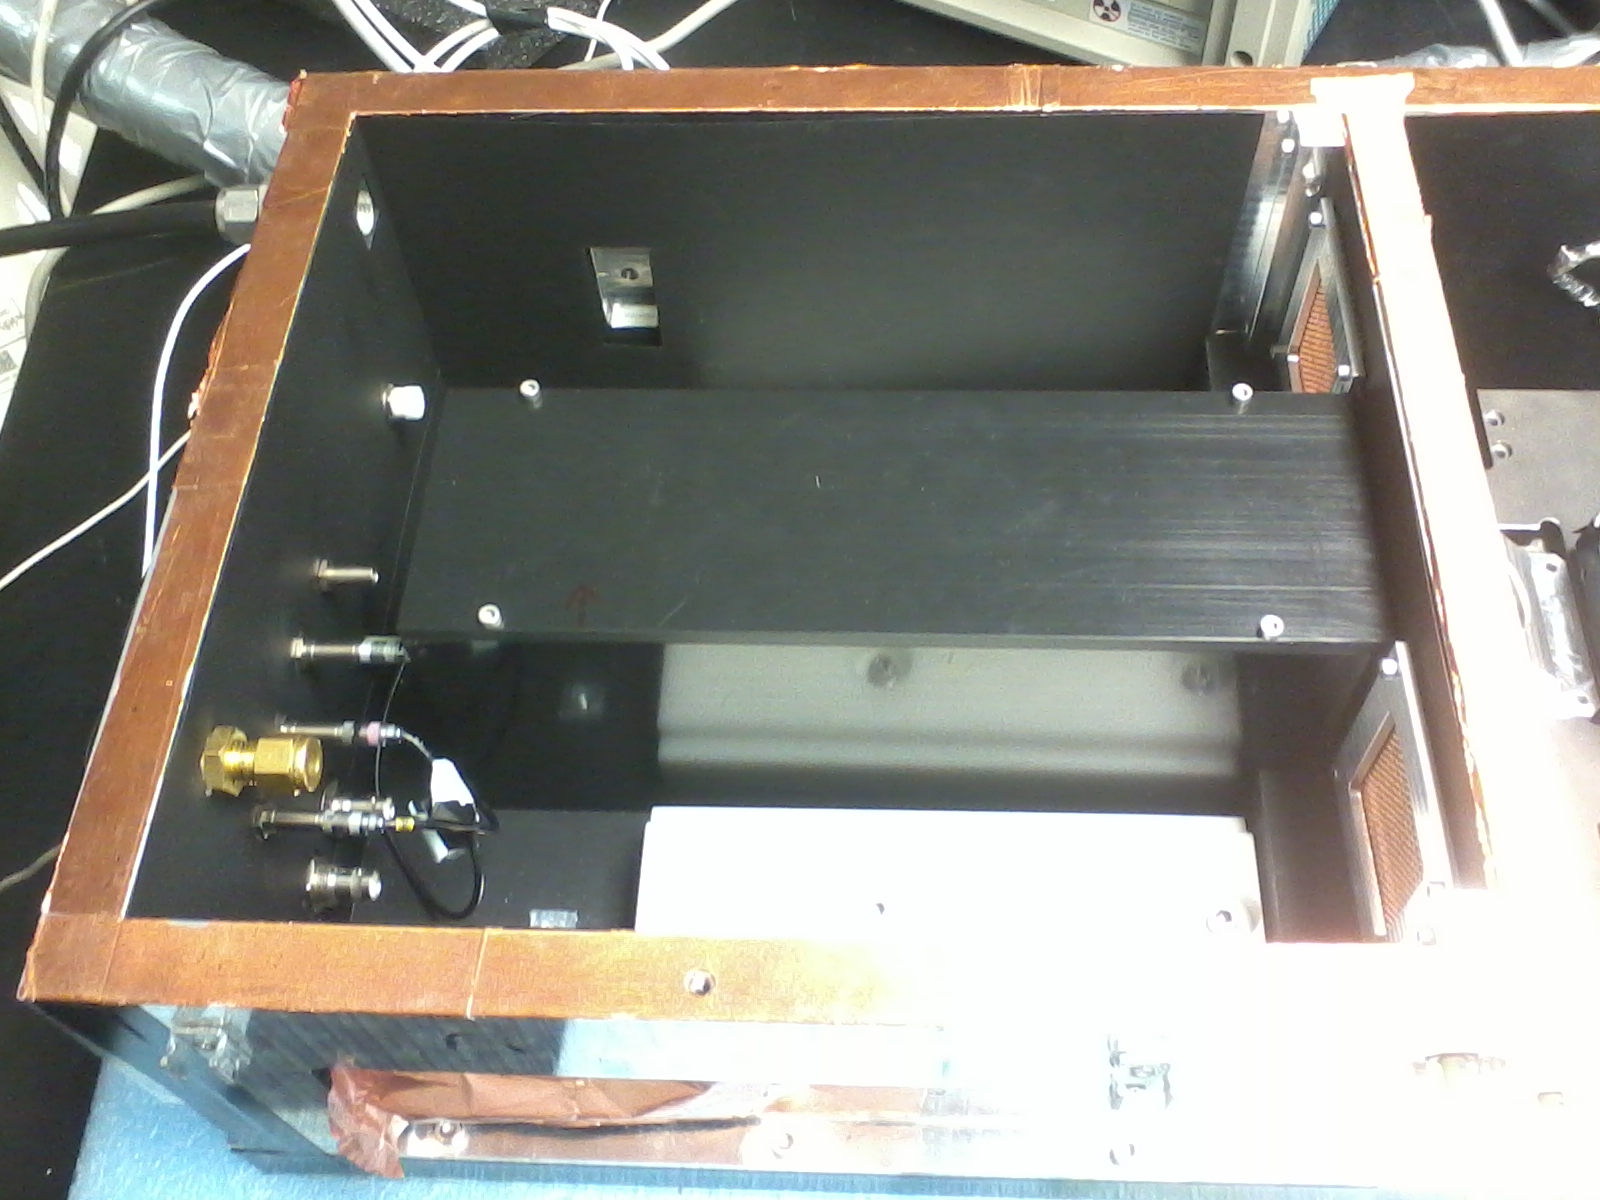
\includegraphics[totalheight=0.4\textwidth,trim=0cm 0cm 0cm 0cm, clip=true]{../Pictures/Pictures_Setup/black_box_lamp.jpg}
    \caption{A black box covering the lamp blocks light leaks from it.}
    \label{fig:black_box}
  \end{figure}
  
  \newpage
  
  Then to absorbe radio frequency leaks from the lamp, 2 pieces of metal are added on the top of that box:
  
  \begin{figure}[!hbtp]
    \centering
    \includegraphics[totalheight=0.4\textwidth,trim=0cm 0cm 0cm 0cm, clip=true]{../Pictures/Pictures_Setup/piece_of_metal.jpg} 
    \caption{Pieces of metal seem to absorbe radio frequency leaks from the lamp.}
    \label{fig:piece_of_metal}
  \end{figure}
  
  
  A photodetector on the bottom can be centered with the hole of 1 mm of the collimator with the help of 2 lines:

  \begin{figure}[!hbtp]
    \centering
    \includegraphics[totalheight=0.4\textwidth,trim=0cm 0cm 0cm 0cm, clip=true]{../Pictures/Pictures_Setup/center_shock.jpg} 
    \caption{These two lines on the shock guide to center the photodetector with the hole of 1 mm of the colllimator.}
    \label{fig:bottom_centered}
  \end{figure}
  
  \newpage
  
  A solution to align properly the photodetector on the top with the hole of 1 mm of the collimator:
  
  \begin{figure}[!hbtp]
    \centering
    \includegraphics[totalheight=0.5\textwidth,trim=5cm 0cm 10cm 0cm, clip=true, angle = 270]{../Pictures/Pictures_Setup/VUV2_top.jpg} 
    \caption{It is quiet difficult to align properly the photodetector of the top with a hole of 1 mm. }
    \label{fig:top_centered}
  \end{figure}
  
  \section{Details about waveforms}
  
  The voltage applied on the lamp makes moves the time of apparition of pulses triggered by photons:
    
  \begin{figure}[!hbtp]
  \centering
    \begin{subfigure}[1.7V.]{%
      \includegraphics[totalheight=.15\textwidth,trim=0.3cm 1.6cm 0.1cm 0cm, clip=true]{../Pictures/Pictures_oscilloscope/17.png} 
      \label{fig:17}}
    \end{subfigure}
  \quad  
    \begin{subfigure}[2.6V.]{%
      \includegraphics[totalheight=.15\textwidth,trim=0.3cm 1.6cm 0.1cm 0cm, clip=true]{../Pictures/Pictures_oscilloscope/26.png}
      \label{fig:26}}
    \end{subfigure}
  \quad  
  \begin{subfigure}[3.6V.]{%
    \includegraphics[totalheight=.15\textwidth,trim=0.3cm 1.6cm 0.1cm 0cm, clip=true]{../Pictures/Pictures_oscilloscope/36.png}
    \label{fig:36}}
  \end{subfigure}
  \quad  
  \begin{subfigure}[4.8V.]{%
    \includegraphics[totalheight=.15\textwidth,trim=0.3cm 1.6cm 0.1cm 0cm, clip=true]{../Pictures/Pictures_oscilloscope/48.png}
    \label{fig:48}}
  \end{subfigure}
  \caption{Increasing the voltage makes appear earlier pulses triggered by photons.}
  \label{fig:17263648}
  \end{figure}
  
  \newpage
  
  To increase the signal from the photo-detectors, two amplifier are used:
  
  \begin{figure}[!hbtp]
    \centering
    \includegraphics[totalheight=0.4\textwidth,trim=9cm 10cm 0cm 0cm, clip=true]{../Pictures/Pictures_Setup/amplifier_1.jpg}
    \caption{Signals from each photo-detector are increased by using amplifiers.}
    \label{fig:amplifier}
  \end{figure}
  
  Difference between photon saturation and electronic saturation:
  
  \begin{figure}[!hbtp]
  \centering  
    \includegraphics[totalheight=.2\textwidth,trim=0.3cm 6.6cm 0.1cm 0cm, clip=true]{../Pictures/Pictures_oscilloscope/saturation_1.png}
    \caption{Electronic saturation from the MEG MPPC.Horizontal axis is 1$\Pmu$s/div and Vertical axis is 1V/div.}
    \label{fig:elec_sat}
  \end{figure}
   
  \begin{figure}[!hbtp]
    \centering
    \includegraphics[totalheight=.2\textwidth,trim=0.3cm 6.6cm 0.1cm 0cm, clip=true]{../Pictures/Pictures_oscilloscope/light_region_2.png}
    \caption{The blue signal shows photon saturation: too many peaks in the 1.4$\Pmu$s region.Horizontal axis is 1$\Pmu$s/div and Vertical axis is 10mV/div.}
    \label{fig:photon_sat}
  \end{figure}

\chapter{Tests}\label{app:tests}

  \section{Attenuation of light}
  
  The optical corporation -Pelham Research Optical LLC - shows in the figure below the coefficient of transmission of the filters used 
  for our setup:
  
  \begin{figure}[!hbtp]
    \centering
    \frame{\includegraphics[totalheight=0.4\textwidth,trim=1.75cm 4.05cm 11.4cm 16.65cm, clip=true, page = 4]{../filter.pdf} }
    \caption{The coefficient of transmission for our filters is less than $20\%$ according to the manufacturer \cite{ref:phelham_filter}.}
    \label{fig:transmissin_filter}
  \end{figure}

    To check that coefficient we calculated the efficiency of a photo-detector on the bottom (VUV2 SiPM), in the same experimental 
    conditions. For the first
    run, the filter was in front of the surface of that photo-detector and for next run, we removed that filter. Then we divided the second 
    result for the efficiency by the first one. That ratio gave us : $18.79\%$.
    \\
    
    Our results are in the file ''$Test_ratio_filter_20\%.ods$`` on GitHub. 
    
  \section{Calibration of temperature sensors}
  
  To calibrate the different temperature sensors used for our setup, we attached each of them on the cooling shock.\\
  Then we set different temperature thanks to the device which allow reaching very low temperature.\\
  Then we recorded each temperature \footnote{Here is the different temperatures: $22.3^\circ C, -0.3^\circ C, -20.3^\circ C, -40.7^\circ C, 
  -60.1^\circ C, 
  -70^\circ C, -80.1^\circ C, -90.2^\circ C, -99.7^\circ C, -110^\circ C$} displays by each of temperature sensors and we 
  obtained one of these figures below:
  
  \begin{figure}[!hbtp]
    \centering
    \includegraphics[totalheight=0.5\textwidth,trim=.5cm 0cm 1.8cm 0.9cm, clip=true]{../Pictures/temp_sensor_2.pdf} 
    \caption{Temperature of one of the sensors versus temperature displays by the cooling system.}
    \label{fig:temp_sensor_2}
  \end{figure}
  
  Taking as reference the temperature displays by the cooling system, after fitting the previous shape, it is now possible to correct 
  each temperature of our sensor, since the equation of the previous fitting is:
  
  \begin{equation}
     Temp_{sensor} = p0\ +\ p1\cdot Temp_{device},
  \end{equation}

  with 
  
  \begin{equation}
     po = -0.379691\   +/-\   0.233424
  \end{equation}
  
  and 
  
  \begin{equation}
    p1 = 1.04282\ +/-\ 0.0033805.
  \end{equation}

 \newpage
 
 \section{Breakdown voltage calculation}
  
  To plot the figure showing the breakdown voltage for the VUV3 SiPM versus temperature \ref{fig:BV_VUV3_SiPM_vs_temp}, here is the method 
  we used to calculate the breakdown voltage of the VUV3 SiPM for different temperatures.
  \\
  
  After setting the desired temperature and triggering on the photo-detector, we took 10 points matching with different voltages and
  we saved 300 waveforms. It was not useful to record more waveforms since the error bars are quiet small (which is not the case for the 
  MEG MPPC). 
  \\
  
  Then the C++ code called ''Normgain.exe' is used to calculate the gain at of the device for the different applied voltages. As the 
  temperature has an influence on the gain, we tried to record all the waveforms at the same temperature \footnote{A variation of temperature
  of $0.2^\circ$ is admissible.} for  such voltages. That is why we registered only 300 waveforms. 
  \\
  
  Then we plotted the calculated gain versus the applied voltages for a desired temperature: 
  
  \begin{figure}[!hbtp]
    \centering
    \includegraphics[totalheight=0.5\textwidth,trim=.5cm 0cm 1.6cm 0.9cm, clip=true]{../Pictures/BV_VUV3_-80C.pdf} 
    \caption{At $-80^\circ$ this figure -gain versus voltage- allow determinate the breakdown voltage thanks to the fitting.}
    \label{fig:BV_VUV3_SiPM}
  \end{figure}
  
  Here is the two parameters obtained from that fitting:
  
  \begin{equation}
    p0\ =\ 4.57394e+01\ +/-\ 3.83652e-02,\ p1\ =\ 1.33438e+02\ +/-\ 1.83935e+00 
  \end{equation}

  \newpage
  
  \section{Error bars calculation}
  
  Here is the error bars calculation
  
  \subsection{PE}
  
  Here is the equation used to calculate the average number of photon electrons $<PE>$:
  
  \begin{equation}
    <PE> =  -ln(\frac{P_{L0}}{P_{D0}}), 
  \end{equation}
 
  where $<PE>$, $P_{L0}$ and $P_{D0}$ are the average number of photon electron, the probability of not observing any pulses in the 
  ``light region'' and in the ``dark region'', respectively.
  \\
  
  Then assuming that the total number of recorded waveforms is $N_{tot}\ =\ 15000$:
  
  \begin{equation}
    \sigma_{P_{L0}}\ =\ \sqrt{\frac{P_{L0}\cdot(1-P_{L0})}{N_{tot}}}
  \end{equation}

  and 
  
  \begin{equation}
    \sigma_{P_{D0}}\ =\ \sqrt{\frac{P_{D0}\cdot(1-P_{D0})}{N_{tot}}}
  \end{equation}
  
  So here is the error bar for the $<PE>$:
  
  \begin{equation}
    \sigma_{<PE>}\ =\ \frac{\sqrt{
    (\frac{\Sigma_{P_{L0}}}{P_{L0}})\textsuperscript{2}\ +\ 
    (\frac{\Sigma_{P_{D0}}}{P_{D0}})\textsuperscript{2}
    }}{N_{tot}}
  \end{equation}
    
  \section{DN}
  
  Here is the equation used to calculate the average number of dark noise $<DN>$:

  \begin{equation}
    <DN> = \ln{\frac{N_{D0}+N_{L0}}{2\cdot15000}},
  \end{equation}

  Lets set:
  
  \begin{equation}
    N_{DN0}\ =\ N_{D0}\ +\ N_{L0},  
  \end{equation}
  
  Thus:
  
  \begin{equation}
    P_{DN0}\ =\ \frac{N_{DN0}}{2\cdot N_{tot}}
  \end{equation}
  
  And:
  
  \begin{equation}
    \sigma_{P_{DN0}}\ =\ \sqrt{\frac{P_{DN0}\cdot(1-P_{DN0})}{2\cdot N_{tot}}}  
  \end{equation}
  
  So here is the error for the $<DN>$:
  
  \begin{equation}
    \sigma_{<DN>}\ =\ \frac{\sigma_{P_{DN0}}}{P_{DN0}}.
  \end{equation}
  
  \section{CT}
  
  Here is the equation used to calculate the average number of crosstalk $<CT>$:
  
  \begin{equation}
    <CT> = -\ln(\frac{N_{1PE}}{N_{>1PE}}),
  \end{equation}  
  
  Thus:
  
  \begin{equation}
    P_{1PE}\ =\ \frac{N_{1PE}}{N_{>1PE}},    
  \end{equation}
  
  Thus:
  
  \begin{equation}
    \sigma_{P_{1PE}}\ =\ \sqrt{\frac{P_{1PE}\cdot(1-P_{1PE})}{N_{>1PE}}}  
  \end{equation}
  
  So here is the error for the $<CT>$:
  
  \begin{equation}
    \sigma_{<CT>}\ =\ \frac{\sigma_{P_{1PE}}}{P_{1PE}}.
  \end{equation}
  
  \section{Test to check light leaks}
  
  To check if we could observe some light leaks from outside of the box, we did a 3 consecutive runs:
  
  \begin{itemize}
   \item Run 1: Lights of the room are off and a black tissue covers the box(black circle),
   \item Run 2: Lights of the room are on and a black tissue covers the box(red triangle),
   \item Run 3: Lights of the room are on and a black tissue is moved from the box (blue lossage).
  \end{itemize}

  \newpage
  
  Plotting next pulses versus time for the same device at the same over-voltage shows clearly light leaks from outside of the box. Indeed the blue 
  lossage doesn't match at all with the first two runs. 
  
  \begin{figure}[!hbtp]
    \centering
    \includegraphics[totalheight=0.7\textwidth,trim=0cm 0cm 1.6cm 0.9cm, clip=true]{../Pictures/DTimeLightLeakAug5.pdf} 
    \caption{Light leaks from outside of the box.}
    \label{fig:light_leaks}
  \end{figure}
  
   
\end{document}

 \section{Efficiency at $-10^\circ$C }
  
  Due to the issue we had with the board at $-100^\circ$C \ref{sec:PE}, we were able to compare the efficiency between the MEG MPPC and 
  the VUV3 SiPM at $-10^\circ$C. At such a temperature, the cooling shock doesn't cool down the board holding the two collimators. 
  \\
  
  The photo-detectro on the top was removed and a UV sensitive PMT is set instaed. Two runs were done in the same experimental conditions:
  position and voltage of the lampe, flux of N2 and number and position of filters. The figure below can show that the quantity of light 
  reaching the PMT is quiet constante over time during the two run. 
  \\
  
  
  
For all our measurements, the position of the lamp and the external voltage were set at 20 mm from the metal divider of the box and 
at 2.8 V, respectively.
  
The absolute efficiency of the photo-detector on the bottom is its own efficiency divided by the efficiency of the photo-detector on the top. 

The probability of observing crosstalk is proportional to the SiPM gain and so to the reversed bias voltage. The same conclusion 
  about the 
  efficiency made in the previous subsection are observed for crosstalk. 
  
At low voltage (2V) the photons are detected after 5$\Pmu$s while at 3V at around 5$\Pmu$s and at 4.8V between 4$\Pmu$s and 4.5$\Pmu$s. 

In the case of dark noise, 
  the first peak of the histogram count the number of time the scope registers zero pulse shape, the second peak matches with the detection of 
  one pulse shape ...
  
  
Pulse shapes triggered by photon have no impact 
  on crosstalk results. Instead of using the second method (trigger on the photo-detector) we could also use the first method (trigger 
  on the lamp) and take in account only the dark region of each waveform.\\